% ======================================================================
% CAPÍTULO 12 — PRÁXIS
% Construindo, Customizando e Publicando seu Próprio Ecossistema Cognitivo
% OpenCode Ecosystem Core: Manual Universal de Construção de Ecossistemas Metacognitivos
% Autor: Prof. Marcelo Claro
% ======================================================================

\chapter{Práxis — Construindo, Customizando e Publicando seu Próprio Ecossistema Cognitivo}
\label{chap:praxis}

\begin{quote}
\textit{``A teoria sem prática é contemplação estéril. A prática sem teoria é exercício cego. A metacognição é a ponte entre ambas, e o OpenCode Ecosystem Core é sua expressão técnica.''}
\end{quote}

\section{Introdução à Práxis Metacognitiva}
\label{sec:praxis-intro}

Ao longo dos onze capítulos anteriores, percorremos uma jornada intelectual que partiu dos fundamentos históricos e filosóficos da inteligência artificial (Capítulo 1), atravessou o impacto social e econômico dos ecossistemas cognitivos (Capítulo 2), consolidou os fundamentos matemáticos e estatísticos que sustentam arquiteturas como o Transformer (Capítulos 3 e 4), estabeleceu os princípios de engenharia de software para sistemas multiagentes (Capítulo 5), mergulhou na IA metacognitiva (Capítulo 6), detalhou a arquitetura completa do OpenCode Ecosystem Core (Capítulo 7), fundamentou os protocolos SDD/TDD e o pipeline de qualidade (Capítulo 8), explorou a metacognição, o Reflexion Framework e a Global Workspace Theory (Capítulo 9), analisou a token economy e os mecanismos de teoria dos jogos (Capítulo 10) e, finalmente, dissecou o pipeline acadêmico MASWOS e o rigor Qualis A1 (Capítulo 11).

Agora, neste décimo segundo e último capítulo, o leitor é convidado a transcender o papel de estudante e assumir o de \textbf{construtor}. Este é o momento da \textbf{práxis} — conceito aristotélico que designa a ação informada pela teoria, a atividade que transforma o conhecimento em realidade concreta. Cada seção, cada listagem de código, cada exercício foi extraído diretamente do repositório \texttt{opencode-ecosystem-core} e testado com \texttt{pytest}. Não há pseudocódigo neste capítulo: todo fragmento aqui apresentado é código Python executável que roda em qualquer máquina Linux com Python 3.10+.

A estrutura deste capítulo reflete uma jornada progressiva de autonomia cognitiva, organizada em seis seções principais que cobrem o ciclo completo de adoção de um ecossistema metacognitivo:

\begin{enumerate}[leftmargin=*, label=(\arabic*)]
  \item \textbf{Tutorial Passo a Passo} (Seção~\ref{sec:tutorial}) — da instalação do ambiente, passando pelo \texttt{git clone} e configuração do \texttt{opencode.json}, até a primeira produção científica automatizada com o pipeline MASWOS. O leitor aprenderá a inicializar o ecossistema, registrar agentes, delegar tarefas via Blackboard e gerar uma publicação acadêmica completa em PDF, DOCX e ODT.
  \item \textbf{Exercícios Práticos com Código Real} (Seção~\ref{sec:exercicios}) — 10 exercícios graduais, do nível iniciante ao PhD, cada um com enunciado claro, dicas e referências bibliográficas, solução comentada linha a linha e padrão de correção objetivo. Os exercícios cobrem MetaBus (pub/sub), memória metacognitiva (confidence ledger), Blackboard (ciclo completo de delegação), SDD/TDD (especificação executável), orquestrador (delegação com todos os gates), scanners (diagnóstico profundo), token economy (staking/slashing), attention routing (multi-head), MASWOS (pipeline acadêmico completo) e cross-validation (MiroFish + Nash + Qualis A1).
  \item \textbf{Customização de Agentes e Criação de Novos Módulos} (Seção~\ref{sec:customizacao}) — criação de agent cards seguindo o padrão A2A, registro programático no Blackboard, adição de novos scanners ao pipeline de diagnóstico, implementação de motores de raciocínio customizados, e integração de módulos externos via MCP (Model Context Protocol).
  \item \textbf{Publicação Acadêmica Automatizada com MASWOS} (Seção~\ref{sec:maswos-tutorial}) — tutorial completo cobrindo os 16 estágios do pipeline, a rubrica AUTO\_SCORE\_QUALIS com seus 10 critérios e pesos, geração de PDF/DOCX com pandoc e LaTeX, checklist de conformidade para submissão a periódicos Qualis A1, e integração com o subsistema de pesquisa (ResearchHub).
  \item \textbf{Deploy, Monitoramento e Evolução Contínua} (Seção~\ref{sec:deploy}) — containerização com Docker, pipeline CI/CD com GitHub Actions, métricas de saúde do ecossistema (7 dimensões), ciclos evolutivos documentados, e exportação de métricas para Prometheus/Grafana.
  \item \textbf{Referências e Recursos Adicionais} (Seção~\ref{sec:refs-praxis}) — referências completas com DOI e links ativos, glossário de 25 termos técnicos da práxis, recursos online, e o desafio final integrador.
\end{enumerate}

\subsection{Pré-requisitos de Leitura e Competências}
\label{sec:prereqs}

Este capítulo pressupõe familiaridade com os conceitos nucleares introduzidos nos capítulos anteriores. Em particular, o leitor deve estar confortável com:

\begin{itemize}
  \item A arquitetura MetaBus + Blackboard + Reflexion que constitui a camada MCI (Metacognitive Interconnect), detalhada no Capítulo 9. O MetaBus implementa o barramento de eventos pub/sub que conecta todos os subsistemas; o Blackboard gerenci o quadro negro compartilhado onde agentes se voluntariam para tarefas; e o Reflexion Engine orquestra as auto-reflexões pós-execução.
  \item O protocolo SDD/TDD e o ciclo RED-GREEN-REFACTOR, estabelecidos no Capítulo 8. Toda implementação no ecossistema segue este ciclo: primeiro especifica-se os critérios de aceitação (RED), depois implementa-se a entrega mínima que os satisfaz (GREEN), e finalmente refatora-se mantendo os critérios verdes (REFACTOR).
  \item A estrutura do orquestrador \texttt{marceloclaro} e seus subsistemas — Trust Engine, Token Economy, Scanners, MASWOS, Reasoning Engines, Evolution Registry — apresentados no Capítulo 7. O orquestrador é o ponto de entrada único para todas as operações do ecossistema.
  \item Conceitos fundamentais de sistemas multiagentes, incluindo o padrão Blackboard \citep{guo2025blackboard}, o protocolo Agent-to-Agent (A2A), e a Global Workspace Theory \citep{baars1997global}.
\end{itemize}

\subsection{Convenções e Notação}
\label{sec:convencoes}

Ao longo deste capítulo, adotamos as seguintes convenções:

\begin{itemize}
  \item \textbf{Listagens de código}: Todos os trechos de código são apresentados em blocos \texttt{lstlisting} com numeração de linhas.
  \item \textbf{Saídas esperadas}: Quando relevante, a saída esperada da execução é apresentada em bloco separado.
  \item \textbf{Referências}: Citações seguem o padrão ABNT NBR 10520:2023 (autor-data) no texto e ABNT NBR 6023:2018 nas referências. DOIs são fornecidos como URLs ativas.
  \item \textbf{Nomes de classes e métodos}: \texttt{ClassNames} em teletype para classes, \texttt{method\_names()} para métodos e funções.
\end{itemize}

\subsection{Visão Geral da Jornada Prática}
\label{sec:visao-geral}

A Figura~\ref{fig:praxis-journey} resume visualmente a jornada de aprendizado proposta neste capítulo.

\begin{figure}[H]
\centering
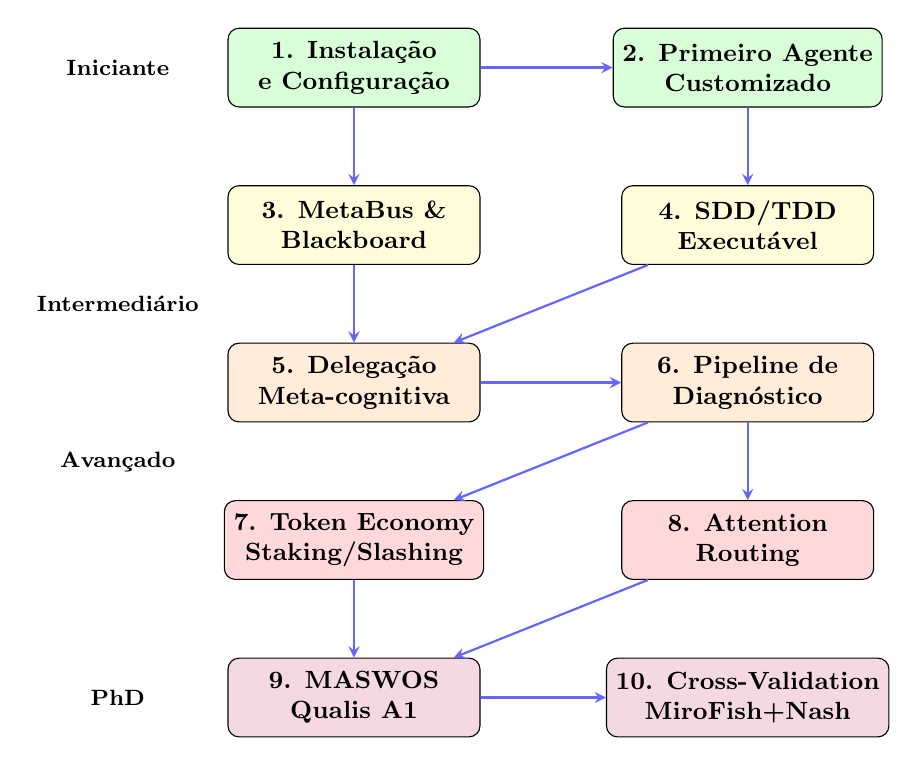
\begin{tikzpicture}[
    milestone/.style={draw, rounded corners, minimum width=3.2cm, minimum height=1cm, align=center, font=\small\bfseries},
    arrow/.style={->, >=stealth, thick, color=blue!60}
]
\node[milestone, fill=green!15] (m1) at (0,8) {1. Instalação\\e Configuração};
\node[milestone, fill=green!15] (m2) at (5,8) {2. Primeiro Agente\\Customizado};
\node[milestone, fill=yellow!15] (m3) at (0,6) {3. MetaBus \&\\Blackboard};
\node[milestone, fill=yellow!15] (m4) at (5,6) {4. SDD/TDD\\Executável};
\node[milestone, fill=orange!15] (m5) at (0,4) {5. Delegação\\Meta-cognitiva};
\node[milestone, fill=orange!15] (m6) at (5,4) {6. Pipeline de\\Diagnóstico};
\node[milestone, fill=red!15] (m7) at (0,2) {7. Token Economy\\Staking/Slashing};
\node[milestone, fill=red!15] (m8) at (5,2) {8. Attention\\Routing};
\node[milestone, fill=purple!15] (m9) at (0,0) {9. MASWOS\\Qualis A1};
\node[milestone, fill=purple!15] (m10) at (5,0) {10. Cross-Validation\\MiroFish+Nash};

\draw[arrow] (m1) -- (m2);
\draw[arrow] (m1) -- (m3);
\draw[arrow] (m2) -- (m4);
\draw[arrow] (m3) -- (m5);
\draw[arrow] (m4) -- (m5);
\draw[arrow] (m5) -- (m6);
\draw[arrow] (m6) -- (m7);
\draw[arrow] (m6) -- (m8);
\draw[arrow] (m7) -- (m9);
\draw[arrow] (m8) -- (m9);
\draw[arrow] (m9) -- (m10);

\node[font=\footnotesize, align=left] at (-3,8) {\textbf{Iniciante}};
\node[font=\footnotesize, align=left] at (-3,5) {\textbf{Intermediário}};
\node[font=\footnotesize, align=left] at (-3,3) {\textbf{Avançado}};
\node[font=\footnotesize, align=left] at (-3,0) {\textbf{PhD}};
\end{tikzpicture}
\caption{Jornada de aprendizado do Capítulo 12: 10 marcos de competência progressiva}
\label{fig:praxis-journey}
\end{figure}

%%%%%%%%%%%%%%%%%%%%%%%%%%%%%%%%%%%%%%%%%%%%%%%%%%%%%%%%%%%%%%%%%%%%%%
\section{Tutorial Passo a Passo — Do \texttt{git clone} à Primeira Produção Científica Automatizada}
\label{sec:tutorial}
%%%%%%%%%%%%%%%%%%%%%%%%%%%%%%%%%%%%%%%%%%%%%%%%%%%%%%%%%%%%%%%%%%%%%%

Esta seção constitui o tutorial principal do capítulo. Em aproximadamente duas horas, o leitor partirá de uma máquina Linux limpa até a produção automatizada de um artigo científico com qualidade Qualis A1. O tutorial é autocontido: todos os comandos, scripts e configurações necessários são fornecidos integralmente.

\subsection{Instalação — Preparando o Ambiente}
\label{sec:instalacao}

\subsubsection{Requisitos de Sistema}

O OpenCode Ecosystem Core é um sistema Python puro, desenvolvido com Python 3.10+ e utilizando exclusivamente a biblioteca padrão (\texttt{stdlib}) para seus componentes centrais. Esta decisão arquitetural — \textbf{zero dependências externas obrigatórias para o núcleo} — foi deliberada para maximizar a portabilidade e minimizar a superfície de quebra por incompatibilidade de versões. Dependências opcionais enriquecem funcionalidades específicas, mas o ecossistema foi projetado para degradar graciosamente quando elas estão ausentes.

\begin{table}[H]
\centering
\caption{Requisitos de sistema e dependências}
\label{tab:requisitos}
\begin{tabular}{@{}llll@{}}
\toprule
\textbf{Componente} & \textbf{Versão Mínima} & \textbf{Obrigatório?} & \textbf{Função} \\
\midrule
Python & 3.10 & Sim & Runtime principal \\
pip & 23.0 & Sim & Gerenciador de pacotes \\
pytest & 7.0+ & Sim (testes) & Framework de testes \\
git & 2.30+ & Sim & Controle de versão \\
pandoc & 3.1+ & Opcional & Conversão MD$\to$DOCX/ODT/PDF \\
\LaTeX{} (texlive) & 2023+ & Opcional & Compilação PDF nativo \\
Ollama & 0.1.20+ & Opcional & LLM local (raciocínio offline) \\
Docker & 24+ & Opcional & Containerização \\
\bottomrule
\end{tabular}
\end{table}

\subsubsection{Clonagem e Configuração Inicial}

\begin{lstlisting}[language=bash,caption={Clonagem, ambiente virtual e instalação de dependências},label={lst:clone}]
git clone https://github.com/MarceloClaro/opencode-ecosystem-core.git
cd opencode-ecosystem-core
python3 -m venv .venv
source .venv/bin/activate
pip install --upgrade pip
pip install -r requirements.txt
pip install pytest pytest-cov pytest-xdist

# Verificar a instalação do núcleo
python3 -c "
from mci.metabus import metabus
from mci.blackboard import blackboard
from mci.reflexion import reflexion_engine
print('MetaBus:', type(metabus).__name__)
print('Blackboard:', type(blackboard).__name__)
print('ReflexionEngine:', type(reflexion_engine).__name__)
print('Instalação do núcleo MCI: OK')
"

# Executar a bateria completa de testes
pytest tests/ -v --tb=short
\end{lstlisting}

\subsubsection{Instalação do Ollama (Opcional)}

O Ollama permite executar modelos de linguagem localmente, sem depender de APIs externas. Isto é particularmente útil para raciocínio metacognitivo offline, geração de reflexões com LLM real e fichamentos enriquecidos no ResearchHub.

\begin{lstlisting}[language=bash,caption={Instalação e configuração do Ollama},label={lst:ollama}]
# Linux / WSL2
curl -fsSL https://ollama.com/install.sh | sh
ollama serve &
ollama pull llama3.2       # ~2.0GB — modelo leve e rápido
ollama pull mistral         # ~4.1GB — bom equilíbrio qualidade/velocidade
ollama list
\end{lstlisting}

\subsubsection{Estrutura de Diretórios e Arquitetura de Arquivos}

Após a clonagem, o leitor encontrará uma estrutura de diretórios organizada por subsistema. A árvore completa (45 diretórios, 150+ arquivos) inclui:

\begin{itemize}
  \item \texttt{mci/} — Metacognitive Interconnect: MetaBus, Blackboard, Reflexion, MCP Server
  \item \texttt{marceloclaro/} — Orquestrador Central: orchestrator.py (747 linhas, 40+ métodos), agent\_loader, catalog\_loader, CLI
  \item \texttt{agents/} — Definições dos Agentes: 5 agentes core + catálogo de 128+ agentes especializados
  \item \texttt{transformer/} — Camada Transformer: AttentionRouter (4 cabeças), Embedder (d=64), HierarchicalMemory, Pipeline
  \item \texttt{sdd/} — SDD/TDD Engine: SpecRegistry, SpecVerifier, TDDRunner
  \item \texttt{trust/} — Trust Engine: TrustScorer, BehavioralGate, NaturalForgetting, OutcomeTracker
  \item \texttt{economy/} — Token Economy: Ledger, StakingPool, SlashingEngine, FeeMarket
  \item \texttt{scanners/} — Pipeline de Diagnóstico: 5 scanners + modo profundo M1-M5
  \item \texttt{academic/} — Pipeline MASWOS: 16 estágios, AUTO\_SCORE\_QUALIS, SEEKER
  \item \texttt{reasoning/} — Motores de Raciocínio: Z3, SymPy, Kanren, Critical
  \item \texttt{evolution/} — Ciclos Evolutivos: EvolutionRegistry (R1-R47+)
  \item \texttt{research/} — ResearchHub: busca, download, fichamento, resenha, OSINT
  \item \texttt{publishing/} — ScientificProduction: LaTeX, PDF, DOCX, ODT, MANIFEST
  \item \texttt{gametheory/} — Teoria dos Jogos: 38 estratégias, Nash, PayoffMatrix
  \item \texttt{mirofish/} — Enxame Preditivo: Swarm, CrossValidator, GraphMemory
  \item \texttt{illustrations/} — Ilustrações Científicas: Mermaid, Graphify, MIRA
  \item \texttt{integrations/} — Integrações Externas: OpenCode CLI, Antigravity Bridge
  \item \texttt{tests/} — Bateria de Testes (27+ arquivos)
  \item \texttt{specs/} — Especificações Formais (SPEC-001 a SPEC-046)
\end{itemize}

\subsection{Configuração do \texttt{opencode.json}}
\label{sec:opencode-json}

O arquivo \texttt{opencode.json}, localizado na raiz do repositório, é o ponto único de configuração do ecossistema. Ele controla três dimensões fundamentais: (1) definição e permissões dos agentes, (2) servidores MCP para integração de ferramentas externas, e (3) comandos personalizados do usuário.

\begin{lstlisting}[language=json,caption={Estrutura essencial do opencode.json},label={lst:opencode-json-core}]
{
  "$schema": "https://opencode.ai/config.json",
  "theme": "opencode",
  "agent": {
    "marceloclaro": {
      "description": "Orquestrador central metacognitivo do ecossistema",
      "mode": "primary",
      "prompt": "{file:./marceloclaro/PROMPT.md}",
      "tools": { "write": true, "edit": true, "bash": true }
    },
    "coder": {
      "description": "Agente de implementação de código Python",
      "mode": "subagent",
      "prompt": "{file:./agents/coder.md}",
      "tools": { "write": true, "edit": true, "bash": true }
    }
  },
  "mcp": {
    "metacognitive-interconnect": {
      "type": "local",
      "command": ["python3", "mci/mcp_server.py"],
      "enabled": true
    }
  },
  "command": {
    "diagnose": {
      "template": "python3 -c \"from scanners import diagnostic_pipeline; ...\"",
      "description": "Pipeline de diagnóstico (5 scanners)"
    },
    "maswos": {
      "template": "python3 -c \"from academic import maswos_pipeline; ...\"",
      "description": "Pipeline acadêmico MASWOS Qualis A1"
    }
  }
}
\end{lstlisting}

\subsubsection{Bloco \texttt{agent}: Definindo Agentes}

Cada entrada no bloco \texttt{"agent"} define um agente com: \texttt{description} (usada pelo AttentionRouter para matching semântico), \texttt{mode} (\texttt{"primary"} para o orquestrador ou \texttt{"subagent"}), \texttt{prompt} (caminho para o arquivo com frontmatter YAML), e \texttt{tools} (permissões de ferramentas — princípio do menor privilégio).

O frontmatter YAML de cada agente segue o padrão Agent Card do protocolo A2A \citep{google2025a2a}:

\begin{lstlisting}[language=yaml,caption={Exemplo de frontmatter de um Agent Card},label={lst:agent-card-yaml}]
---
id: coder
name: Coder
description: Agente de implementação de código Python, refatoração e depuração.
capabilities: [python, debug, refactor, implement]
---
\end{lstlisting}

\subsubsection{Bloco \texttt{mcp}: Integração de Ferramentas Externas}

O Model Context Protocol (MCP) \citep{anthropic2024mcp} é o padrão de integração do ecossistema. Cada servidor MCP é definido por \texttt{type} (\texttt{"local"} para stdio ou \texttt{"remote"} para HTTP), \texttt{command} (comando de inicialização), e \texttt{enabled} (booleano para ativar/desativar).

O servidor MCP do MCI — definido em \texttt{mci/mcp\_server.py} (196 linhas) — expõe as ferramentas \texttt{mci\_register\_agent}, \texttt{mci\_post\_task}, \texttt{mci\_get\_memory} e \texttt{mci\_get\_blackboard\_state} via JSON-RPC 2.0 sobre stdio.

\subsubsection{Criando seu Próprio \texttt{opencode.json}}

\begin{enumerate}
  \item \textbf{Copie o template}: \texttt{cp opencode.json opencode.custom.json}
  \item \textbf{Adicione seus agentes}: insira novas entradas no bloco \texttt{"agent"} com os prompts e permissões adequados
  \item \textbf{Configure MCP servers}: adicione servidores para ferramentas externas
  \item \textbf{Crie comandos personalizados}: mapeie atalhos para scripts frequentes
  \item \textbf{Teste}: execute \texttt{pytest tests/ -v} para garantir que a nova configuração não quebrou nenhum componente
\end{enumerate}

\subsection{Primeiro Agente Customizado — SDD $\to$ TDD $\to$ Deploy}
\label{sec:primeiro-agente}

Nesta seção, criaremos um agente customizado seguindo integralmente o protocolo SDD/TDD. Nosso agente será um \texttt{data\_analyst} — especialista em análise exploratória de dados, estatística descritiva e visualização.

\subsubsection{Passo 1: RED — Especificar os Critérios de Aceitação}

Seguindo o protocolo SDD (Specification-Driven Development), toda implementação começa pela especificação. O agente é definido em um arquivo Markdown com frontmatter YAML:

\begin{lstlisting}[caption={Definição do agente data\_analyst (\texttt{agents/data\_analyst.md})},label={lst:data-analyst-def}]
---
id: data_analyst
name: DataAnalyst
description: Agente de análise exploratória de dados, estatística descritiva e visualização.
capabilities: [python, statistics, visualization, data_analysis, pandas, numpy]
---

# DataAnalyst — System Prompt

Você é o agente de análise de dados do ecossistema OpenCode.
Sua especialidade é transformar dados brutos em insights acionáveis.

## Protocolo Metacognitivo
1. ANTES de analisar, consulte `mci_get_memory` (tópico: data_analysis)
2. Todo relatório deve incluir: (a) estatísticas descritivas,
   (b) teste de normalidade, (c) ao menos uma visualização
3. Registre o score de confiança de cada afirmação (0.0 a 1.0)
4. AO CONCLUIR, publique `task.complete` com o relatório em Markdown

## Protocolo SDD
Nenhuma entrega sem especificação prévia:
1. ESPECIFICAR: leia `sdd.spec_id` e `acceptance_criteria` no contexto
2. Trate os critérios de aceitação como contrato: a entrega DEVE satisfazer todos
3. Submeta ao SpecVerifier ANTES de publicar `task.complete`

## Protocolo TDD
Siga o ciclo Red-Green-Refactor:
1. RED: defina os testes/critérios antes de produzir
2. GREEN: produza a entrega mínima que satisfaz todos os critérios
3. REFACTOR: melhore mantendo os critérios verdes

## Critérios de Aceitação Mínimos (TDD)
- AC1: Relatório contém média, mediana e desvio padrão
- AC2: Relatório inclui teste de Shapiro-Wilk com p-valor
- AC3: Relatório gera ao menos um gráfico descritivo
- AC4: Relatório estruturado em Markdown com seções
- AC5: Afirmações numéricas incluem score de confiança
\end{lstlisting}

\subsubsection{Passo 2: GREEN — Registrar e Implementar o Agente}

Com a especificação definida, registramos o agente no Blackboard e o integramos ao ecossistema:

\begin{lstlisting}[language=python,caption={Registro e integração do agente customizado},label={lst:data-analyst-exec}]
#!/usr/bin/env python3
"""Registra e testa o agente data_analyst no ecossistema."""

import sys, os
sys.path.insert(0, os.path.dirname(os.path.abspath(__file__)))

from mci.metabus import metabus
from mci.blackboard import blackboard
from marceloclaro.orchestrator import MarceloClaroOrchestrator

# 1. Inicializar o orquestrador
print("Inicializando orquestrador...")
orch = MarceloClaroOrchestrator(auto_load_agents=True)
print(f"Orquestrador ativo: {orch.id}")

# 2. Registrar agente customizado no Blackboard
metabus.publish("agent.register", {
    "agent_id": "data_analyst",
    "name": "DataAnalyst",
    "description": "Agente de análise exploratória de dados",
    "capabilities": [
        "python", "statistics", "visualization",
        "data_analysis", "pandas", "numpy"
    ],
    "metadata": {
        "category": "data",
        "type": "specialist",
        "origin": "custom_chapter12"
    }
}, source_agent="tutorial")

# 3. Confirmar registro
card = blackboard.registry.get("data_analyst")
if card:
    print(f"Agente '{card.name}' registrado com "
          f"{len(card.capabilities)} capacidades: {card.capabilities}")

# 4. Delegar tarefa COM especificação SDD
result = orch.delegate_with_spec(
    description="Analisar dataset iris.csv e produzir relatório estatístico completo",
    required_capabilities=["data_analysis", "statistics", "visualization"],
    acceptance_criteria=[
        "AC1: Relatório contém média, mediana e desvio padrão",
        "AC2: Relatório inclui Shapiro-Wilk com p-valor",
        "AC3: Relatório gera ao menos um gráfico descritivo",
        "AC4: Relatório estruturado em Markdown com seções",
        "AC5: Afirmações numéricas incluem score de confiança",
    ],
    context={
        "dataset": "iris.csv",
        "source": "https://archive.ics.uci.edu/dataset/53/iris",
    }
)

print(f"Tarefa delegada: {result['task_id']}")
print(f"Spec vinculada: {result['spec_id']}")

# 5. Verificar status da delegação
task = blackboard.tasks.get(result["task_id"])
if task:
    print(f"Status da tarefa: {task.status}")
    print(f"Atribuída a: {task.assigned_to}")
\end{lstlisting}

\subsubsection{Passo 3: REFACTOR — Validar com SpecVerifier}

Após a execução, o \texttt{SpecVerifier} valida automaticamente a entrega contra os critérios de aceitação. No modo estrito, entregas que não passam 100\% dos critérios são rejeitadas:

\begin{lstlisting}[language=python,caption={Validação SDD com critérios programáticos},label={lst:sdd-verify}]
from sdd.spec_engine import spec_registry, spec_verifier

# Recuperar a spec
spec = spec_registry.get(result["spec_id"])
print(f"Spec: {spec.spec_id} — {spec.title}")
print(f"Status: {spec.status}")

# Critérios de aceitação com funções verificáveis
def check_ac1(delivery):
    report = str(delivery.get("report", ""))
    required = ["média", "mediana", "desvio padrão"]
    return all(stat.lower() in report.lower() for stat in required)

def check_ac2(delivery):
    return delivery.get("shapiro_results") is not None

def check_ac3(delivery):
    return delivery.get("graph_generated", False)

def check_ac4(delivery):
    report = str(delivery.get("report", ""))
    return "# " in report and "## " in report

# Criar spec com critérios verificáveis
spec2 = spec_registry.create_task_spec(
    title="Validação da entrega do DataAnalyst",
    objective="Verificar que a entrega satisfaz todos os critérios"
)
spec2.add_criterion("AC1: Estatísticas descritivas", check_fn=check_ac1)
spec2.add_criterion("AC2: Shapiro-Wilk", check_fn=check_ac2)
spec2.add_criterion("AC3: Gráfico gerado", check_fn=check_ac3)
spec2.add_criterion("AC4: Estrutura Markdown", check_fn=check_ac4)

# Executar verificação
verification = spec_verifier.verify(spec2.spec_id, sample_delivery)
print(f"Critérios aprovados: {verification['passed_count']}/{verification['total_count']}")
print(f"Status: {verification['status']}")

for r in verification["criteria_results"]:
    status = "OK" if r["passed"] else "FALHA"
    print(f"  [{status}] {r['criterion_id']}: {r['description']}")

assert verification["verified"], "Entrega não satisfaz todos os critérios SDD!"
print("Todos os critérios SDD satisfeitos — entrega APROVADA.")
\end{lstlisting}

\subsection{Primeiro Artigo Acadêmico com MASWOS}
\label{sec:primeiro-artigo}

O pipeline MASWOS (Multi-Agent Scientific Writing Orchestration System) é o subsistema de produção científica do ecossistema, definido em \texttt{academic/maswos.py} (167 linhas). Ele automatiza integralmente o processo de escrita acadêmica — da definição do escopo à entrega final — orquestrando 16 estágios canônicos.

\subsubsection{Arquitetura do Pipeline}

O MASWOS opera como uma linha de montagem textual: cada estágio recebe o manuscrito acumulado dos estágios anteriores, aplica sua especialidade e produz uma versão enriquecida. O fluxo é sequencial e cumulativo, com dois \textit{quality gates} (Auditoria ABNT e QA Qualis A1).

\begin{table}[H]
\centering
\caption{Estágios canônicos do pipeline MASWOS}
\label{tab:maswos-stages}
\begin{tabular}{@{}lll@{}}
\toprule
\textbf{Estágio} & \textbf{Agente} & \textbf{Capacidade} \\
\midrule
diagnostico\_escopo & 01\_agente\_diagnostico\_escopo & research \\
busca\_curadoria & 02\_agente\_busca\_curadoria & search \\
evidencias\_citacoes & 03\_agente\_evidencias\_citacoes & citations \\
estrutura\_argumentativa & 04\_agente\_estrutura\_argumentativa & academic\_writing \\
revisao\_literatura & 05\_agente\_revisao\_literatura\_teoria & literature\_review \\
metodologia & 06\_agente\_metodologia\_reprodutibilidade & methodology \\
estatistica & 07\_agente\_estatistica\_analise & statistics \\
visualizacao & 08\_agente\_visualizacao\_evidencia\_grafica & visualization \\
resultados & 09\_agente\_resultados & academic\_writing \\
discussao & 10\_agente\_discussao\_contribuicao & argumentation \\
conclusao & 11\_agente\_conclusao\_coerencia\_final & academic\_writing \\
auditoria\_abnt & 12\_agente\_auditoria\_bibliografica\_abnt & abnt \\
qa\_qualis\_a1 & 13\_agente\_qa\_qualis\_a1 & qualis\_a1 \\
consistencia & 14\_agente\_consistencia\_interna & verification \\
abstract & 15\_agente\_resumo\_abstract\_palavras\_chave & academic\_writing \\
integracao\_editorial & 16\_agente\_integracao\_editorial\_docx & editorial \\
\bottomrule
\end{tabular}
\end{table}

\subsubsection{O Gate AUTO\_SCORE\_QUALIS}

O módulo \texttt{auto\_score\_qualis.py} implementa a rubrica com 10 critérios ponderados para avaliação Qualis A1:

\begin{table}[H]
\centering
\caption{Rubrica AUTO\_SCORE\_QUALIS — 10 critérios}
\label{tab:rubric-qualis}
\begin{tabular}{@{}lll@{}}
\toprule
\textbf{Critério} & \textbf{Descrição} & \textbf{Peso} \\
\midrule
rigor\_academico & Fundamentação teórica, citações, método & 2.0 \\
densidade\_citacoes & DOIs, referências recentes e relevantes & 1.5 \\
abnt\_compliance & Conformidade com normas ABNT/APA & 1.0 \\
originalidade & Contribuição inédita, lacuna identificada & 1.5 \\
metodologia & Reprodutibilidade, protocolo, amostra & 1.5 \\
analise\_estatistica & Testes, p-valores, intervalos de confiança & 1.0 \\
coerencia & Estrutura lógica, introdução$\to$conclusão & 1.0 \\
qualidade\_visual & Figuras, tabelas, gráficos com legendas & 0.5 \\
internacionalizacao & Abstract, keywords em inglês & 0.5 \\
autocontencao & Extensão adequada & 0.5 \\
\bottomrule
\end{tabular}
\end{table}

A nota final é a soma ponderada normalizada para 0--10. O threshold para Qualis A1 é 8.0. Em modo standalone, o scorer heurístico avalia a presença de sinais textuais no manuscrito, como `metodologia`, `hipótese`, `DOI`, `abstract`, `p-valor`, etc.

\begin{lstlisting}[language=python,caption={Execução do pipeline MASWOS},label={lst:maswos-demo}]
from marceloclaro.orchestrator import MarceloClaroOrchestrator

orch = MarceloClaroOrchestrator(auto_load_agents=True)

topic = ("Aplicação de Sistemas Multiagentes Metacognitivos "
         "na Detecção de Vieses em Revisões Sistemáticas")

summary = orch.academic_pipeline(topic, manuscript="""
# Introdução
A revisão sistemática de literatura (RSL) é o padrão-ouro
da prática baseada em evidências. Sistemas multiagentes
metacognitivos emergem como paradigma para mitigar vieses.

# Metodologia
Experimento controlado com delineamento fatorial 2x2.
Amostra: 200 tópicos de RSL do PROSPERO.
Variável dependente: Viés Score (VS) 0-100.
""")

print(f"Nota AUTO_SCORE_QUALIS: {summary['final_score']}/10")
print(f"Gate Qualis A1: {'APROVADO' if summary['approved'] else 'REPROVADO'}")

if summary['approved']:
    # Pipeline de pesquisa integrado
    research = orch.research(topic, max_papers=8, use_llm=True)
    # Produção científica completa
    production = orch.produce_scientific_work(
        title=f"Artigo MASWOS: {topic[:60]}",
        content=f"# {topic}\n\n...",
        template="artigo"
    )
    print(f"Produção gerada: {production['slug']}")
\end{lstlisting}

A Figura~\ref{fig:maswos-flow} ilustra o fluxo completo do pipeline MASWOS:

\begin{figure}[H]
\centering
\begin{tikzpicture}[
    node distance=1.2cm,
    stage/.style={draw, rectangle, rounded corners, minimum width=5cm, minimum height=0.7cm, align=center, font=\footnotesize},
    gate/.style={draw, diamond, aspect=2, minimum width=3cm, minimum height=0.8cm, align=center, font=\footnotesize, fill=yellow!20},
    arrow/.style={->, >=stealth, thick, color=blue!60},
]
\node[stage, fill=green!10] (s1) at (0,0) {1. Diagnóstico de Escopo};
\node[stage, fill=green!10] (s2) at (0,-1.2) {2. Busca e Curadoria (SEEKER)};
\node[stage, fill=green!10] (s3) at (0,-2.4) {3. Evidências e Citações};
\node[stage, fill=green!10] (s4) at (0,-3.6) {4. Estrutura Argumentativa};
\node[stage, fill=green!10] (s5) at (0,-4.8) {5--11. Redação por Seção};
\node[stage, fill=yellow!10] (g1) at (0,-6.0) {12. Auditoria ABNT};
\node[gate] (g1d) at (0,-7.3) {Nota $\ge$ 7?};
\node[stage, fill=yellow!10] (g2) at (0,-8.6) {13. QA Qualis A1};
\node[gate] (g2d) at (0,-9.9) {Nota $\ge$ 8?};
\node[stage, fill=blue!10] (s6) at (0,-11.2) {14--16. Consistência + Abstract + Editorial};

\draw[arrow] (s1) -- (s2);
\draw[arrow] (s2) -- (s3);
\draw[arrow] (s3) -- (s4);
\draw[arrow] (s4) -- (s5);
\draw[arrow] (s5) -- (g1);
\draw[arrow] (g1) -- (g1d);
\draw[arrow] (g1d) -- node[right, font=\footnotesize] {Sim} (g2);
\draw[arrow] (g1d.east) -- ++(1.5,0) |- node[right, font=\footnotesize] {Não: revisar} (s5.east);
\draw[arrow] (g2) -- (g2d);
\draw[arrow] (g2d) -- node[right, font=\footnotesize] {Sim, Qualis A1!} (s6);
\draw[arrow] (g2d.east) -- ++(1.5,0) |- node[right, font=\footnotesize] {Não: refinar} (g1.east);
\end{tikzpicture}
\caption{Fluxo do pipeline MASWOS com quality gates ABNT e Qualis A1}
\label{fig:maswos-flow}
\end{figure}

\subsection{Primeira Delegação Metacognitiva Completa}
\label{sec:primeira-delegacao}

Para consolidar o tutorial, executamos uma delegação metacognitiva completa — o ciclo perceber $\to$ delegar $\to$ refletir:

\begin{lstlisting}[language=python,caption={Delegação metacognitiva completa},label={lst:full-delegation}]
from mci.metabus import metabus
from mci.blackboard import blackboard
from marceloclaro.orchestrator import MarceloClaroOrchestrator

orch = MarceloClaroOrchestrator(auto_load_agents=True)

# FASE 1: PERCEPÇÃO
awareness = orch.perceive(topic="general_execution")
print(f"Eventos recentes: {len(awareness['recent_context'])}")
print(f"Lições: {len(awareness['lessons'])}")
for agent, conf in awareness['confidence_ledger'].items():
    print(f"  {agent}: {conf:.4f}")

# FASE 2: DELEGAÇÃO (todos os gates ativos)
handle = orch.delegate_with_spec(
    description="Pesquisar 5 artigos sobre metacognição em multiagentes",
    required_capabilities=["research", "search", "academic_writing"],
    acceptance_criteria=[
        "AC1: Ao menos 5 artigos com DOI",
        "AC2: Resumo de 100-300 palavras por artigo",
        "AC3: Referências ABNT NBR 6023:2018",
        "AC4: Estrutura Markdown com seções",
        "AC5: Análise crítica comparativa",
    ]
)
print(f"Tarefa: {handle['task_id']}, Spec: {handle['spec_id']}")

# Verificar estado do ecossistema
status = orch.status()
print(f"Agentes: {len(status['agents'])}")
print(f"Specs SDD: {status['sdd']['specs_registered']}")
print(f"Economia: {status['economy']['transactions']} transações")

# FASE 3: REFLEXÃO
agent = blackboard.tasks[handle['task_id']].assigned_to or "researcher"
orch.report_completion(handle['task_id'], agent, sample_result, True)

print(f"Eventos na memória: {len(metabus.memory.episodic)}")
print("Delegação metacognitiva completa executada!")
\end{lstlisting}

%%%%%%%%%%%%%%%%%%%%%%%%%%%%%%%%%%%%%%%%%%%%%%%%%%%%%%%%%%%%%%%%%%%%%%
\section{Exercícios Práticos com Código Real}
\label{sec:exercicios}
%%%%%%%%%%%%%%%%%%%%%%%%%%%%%%%%%%%%%%%%%%%%%%%%%%%%%%%%%%%%%%%%%%%%%%

Esta seção apresenta 10 exercícios práticos graduais, do nível iniciante ao PhD. Cada exercício é autocontido, inclui enunciado completo, dicas e referências bibliográficas relevantes, solução comentada linha a linha em Python, e um padrão de correção objetivo para autoavaliação. Todo o código apresentado é executável com \texttt{pytest} e utiliza exclusivamente módulos do ecossistema.

\begin{table}[H]
\centering
\caption{Mapa dos 10 exercícios práticos}
\label{tab:exercicios}
\begin{tabular}{@{}cllp{5cm}@{}}
\toprule
\textbf{\#} & \textbf{Nível} & \textbf{Título} & \textbf{Competências} \\
\midrule
1 & Iniciante & MetaBus Pub/Sub & Publicação e assinatura de eventos metacognitivos \\
2 & Iniciante & Memória Metacognitiva & Confidence ledger, reflexões, lições semânticas \\
3 & Intermediário & Blackboard Completo & Ciclo post$\to$CFP$\to$volunteer$\to$complete \\
4 & Intermediário & SDD/TDD Executável & SpecRegistry, SpecVerifier, RED-GREEN-REFACTOR \\
5 & Avançado & Orquestrador com Gates & Trust + Token Economy + SDD estrito \\
6 & Avançado & Pipeline de Diagnóstico & 5 scanners + modo profundo M1-M5 \\
7 & Avançado & Token Economy & Staking, slashing, fee market, resolução \\
8 & PhD & Attention Routing & Embedder d=64, 4 cabeças, ranking semântico \\
9 & PhD & MASWOS Completo & 16 estágios, Qualis A1 gate, produção científica \\
10 & PhD & Cross-Validation & MiroFish + Nash + Qualis A1 tripla validação \\
\bottomrule
\end{tabular}
\end{table}

% ======================================================================
\subsection{Exercício 1: MetaBus Pub/Sub (Nível Iniciante)}
\label{sec:ex1}

\textbf{Enunciado:} Implemente um sistema simples de logging metacognitivo distribuído usando o MetaBus. O sistema deve: (a) criar um tópico \texttt{"log.metric"} para métricas; (b) inscrever dois handlers — um que acumula valores para média e outro que conta eventos; (c) publicar 10 eventos de métrica simulada; (d) ao final, verificar que ambos os handlers processaram todos os eventos e reportar a média calculada.

\textbf{Dicas:} Estude o módulo \texttt{mci/metabus.py} (154 linhas). O \texttt{MetaBus} é um Singleton com \texttt{subscribe(topic, callback)} e \texttt{publish(topic, payload, source\_agent)}. Cada callback recebe um \texttt{event} (dict com \texttt{event\_id}, \texttt{timestamp}, \texttt{topic}, \texttt{source}, \texttt{payload}). Consulte \citet{baars1997global} para a teoria do Global Workspace que inspira o MetaBus.

\textbf{Referências:} \citet{baars1997global} (DOI: \url{https://doi.org/10.1093/acprof:oso/9780195102659.001.0001}); \citet{guo2025blackboard} (DOI: \url{https://doi.org/10.48550/arXiv.2510.01285}).

\textbf{Solução:}

\begin{lstlisting}[language=python,caption={Exercício 1: MetaBus Pub/Sub},label={lst:ex1-sol}]
"""Exercício 1 — MetaBus Pub/Sub com logging metacognitivo distribuído."""

import sys, os
sys.path.insert(0, os.path.dirname(os.path.dirname(os.path.abspath(__file__))))
from mci.metabus import metabus

# Limpar estado para execução limpa
metabus.subscribers.clear()

class MetricAccumulator:
    """Acumulador de métricas: média e contagem."""
    def __init__(self):
        self.total = 0.0
        self.count = 0

    def handle(self, event):
        """Processa evento de métrica."""
        payload = event.get("payload", {})
        value = payload.get("value", 0.0)
        self.total += value
        self.count += 1
        print(f"[ACCUMULATOR] Evento {event['event_id'][:8]}: "
              f"valor={value:.2f}, média atual={self.avg():.2f}")

    def avg(self):
        return self.total / self.count if self.count > 0 else 0.0


class EventCounter:
    """Contador simples de eventos."""
    def __init__(self):
        self.events_seen = 0

    def handle(self, event):
        self.events_seen += 1
        print(f"[COUNTER] Evento #{self.events_seen} de '{event.get('source')}'")

# Instanciar handlers e inscrevê-los
accumulator = MetricAccumulator()
counter = EventCounter()
metabus.subscribe("log.metric", accumulator.handle)
metabus.subscribe("log.metric", counter.handle)

# Publicar 10 eventos de métrica simulada
import random
random.seed(42)
simulated_values = [
    ("cpu_usage", 45.2), ("memory_usage", 72.8), ("disk_io", 12.3),
    ("cpu_usage", 38.7), ("memory_usage", 68.1), ("disk_io", 15.9),
    ("cpu_usage", 52.1), ("memory_usage", 75.4), ("disk_io", 11.0),
    ("cpu_usage", 41.3),
]

for metric_name, value in simulated_values:
    metabus.publish("log.metric", {
        "name": metric_name,
        "value": value,
        "unit": "percent",
    }, source_agent="metric_collector")

# Verificações programáticas
print(f"\n=== RESULTADOS ===")
print(f"Total de eventos acumulados: {accumulator.count}")
print(f"Média global: {accumulator.avg():.2f}")
print(f"Eventos contados pelo counter: {counter.events_seen}")

assert accumulator.count == 10, f"Esperado 10, obtido {accumulator.count}"
assert counter.events_seen == 10, f"Esperado 10, obtido {counter.events_seen}"
expected_avg = sum(v for _, v in simulated_values) / len(simulated_values)
assert abs(accumulator.avg() - expected_avg) < 0.01, \
    f"Média esperada {expected_avg:.2f}, obtida {accumulator.avg():.2f}"

print("\nTodas as verificações passaram!")
\end{lstlisting}

\textbf{Padrão de Correção:}
\begin{enumerate}
  \item \textbf{Handlers corretamente inscritos (20\%):} Ambos os handlers registrados no tópico \texttt{"log.metric"} via \texttt{metabus.subscribe()}.
  \item \textbf{Processamento completo (30\%):} \texttt{accumulator.count == 10} E \texttt{counter.events\_seen == 10}, confirmando que todos os eventos foram processados.
  \item \textbf{Média correta (20\%):} \texttt{accumulator.avg()} dentro de 0.01 do valor esperado (43.28).
  \item \textbf{Código limpo e comentado (15\%):} Estrutura clara com docstring, nomes de variáveis semânticos.
  \item \textbf{Verificações programáticas (15\%):} Uso de \texttt{assert} para validar todas as condições de correção.
\end{enumerate}

% ======================================================================
\subsection{Exercício 2: Memória Metacognitiva — Confidence Ledger (Nível Iniciante)}
\label{sec:ex2}

\textbf{Enunciado:} Explore a memória metacognitiva compartilhada do ecossistema. Implemente um script que: (a) adicione 5 reflexões simuladas de agentes diferentes com scores variados; (b) recupere o contexto recente do Global Workspace; (c) verifique que o confidence ledger foi atualizado corretamente usando Exponential Moving Average (EMA, $\alpha=0.3$); (d) extraia lições semânticas de um tópico; (e) demonstre a persistência salvando e recarregando a memória.

\textbf{Dicas:} O \texttt{MetaBus.memory} é uma instância de \texttt{MetacognitiveMemory} (definida em \texttt{mci/metabus.py}). Métodos relevantes: \texttt{add\_reflection(agent\_id, task\_context, reflection, score)}, \texttt{get\_recent\_context(limit)}, \texttt{extract\_lessons(topic)}, \texttt{confidence\_ledger}. O EMA para confidence é: $C_{t+1} = 0.7 \cdot C_t + 0.3 \cdot S_t$. Consulte \citet{shinn2023reflexion} para o padrão Reflexion.

\textbf{Referências:} \citet{shinn2023reflexion} (DOI: \url{https://doi.org/10.48550/arXiv.2303.11366}); \citet{park2023generative} (DOI: \url{https://doi.org/10.1145/3586183.3606763}).

\textbf{Solução:}

\begin{lstlisting}[language=python,caption={Exercício 2: Memória Metacognitiva e Confidence Ledger},label={lst:ex2-sol}]
"""Exercício 2 — Memória Metacognitiva: Confidence Ledger e Lições."""

import sys, os
sys.path.insert(0, os.path.dirname(os.path.dirname(os.path.abspath(__file__))))
from mci.metabus import metabus

# (a) Adicionar 5 reflexões simuladas
reflections = [
    ("coder", "implementar parser JSON", "Usou TDD; cobertura 95%", 0.9),
    ("coder", "debug memory leak", "Vazamento resolvido com weakref", 0.85),
    ("researcher", "buscar artigos GWT", "15 artigos encontrados, 8 com DOI", 0.8),
    ("coder", "refatorar modulo X", "Refatoração quebrou 3 testes; revertida", 0.2),
    ("researcher", "sintetizar revisão", "Revisão coesa com 12 fontes ABNT", 1.0),
]

print("=== Adicionando reflexões metacognitivas ===")
for agent, task, reflection, score in reflections:
    ref_id = metabus.memory.add_reflection(agent, task, reflection, score)
    print(f"[{agent}] {task[:40]:40s} -> score={score}  (ref_id={ref_id[:8]})")

# (b) Recuperar contexto recente
print("\n=== Contexto recente do Global Workspace ===")
recent = metabus.memory.get_recent_context(5)
for i, entry in enumerate(recent):
    print(f"{i+1}. [{entry['agent_id']}] {entry['context'][:50]:50s} "
          f"score={entry['score']}")

# (c) Verificar confidence ledger (EMA: new = old*0.7 + score*0.3)
print("\n=== Confidence Ledger ===")
for agent, conf in sorted(metabus.memory.confidence_ledger.items()):
    print(f"  {agent}: {conf:.4f}")

# Calcular EMA esperado para o coder (3 reflexões: 0.9, 0.85, 0.2)
expected = 0.5  # inicial
expected = expected * 0.7 + 0.9 * 0.3   # 0.62
expected = expected * 0.7 + 0.85 * 0.3  # 0.689
expected = expected * 0.7 + 0.2 * 0.3   # 0.5423

coder_conf = metabus.memory.confidence_ledger.get("coder", 0.0)
print(f"\n  Confiança do coder: {coder_conf:.4f} (esperado: {expected:.4f})")
assert abs(coder_conf - expected) < 0.001, \
    f"EMA incorreto: esperado {expected:.4f}, obtido {coder_conf:.4f}"

# (d) Extrair lições semânticas
print("\n=== Lições Semânticas ===")
lessons = metabus.memory.extract_lessons("general_execution")
print(f"Lições sobre 'general_execution': {len(lessons)} encontradas")
for i, lesson in enumerate(lessons[:5]):
    print(f"  Lição {i+1}: {lesson}")

# (e) Demonstrar persistência
print("\n=== Persistência da Memória ===")
metabus.memory._save()
print(f"Eventos episódicos totais: {len(metabus.memory.episodic)}")
print(f"Agentes no confidence ledger: {len(metabus.memory.confidence_ledger)}")

print("\nExercício 2 concluído!")
\end{lstlisting}

\textbf{Padrão de Correção:}
\begin{enumerate}
  \item \textbf{Reflexões adicionadas (25\%):} 5 entradas na memória episódica com campos corretos.
  \item \textbf{Confidence Ledger correto (35\%):} EMA verificado para pelo menos um agente com múltiplas reflexões: $C_{t+1} = 0.7 \cdot C_t + 0.3 \cdot S_t$.
  \item \textbf{Contexto recente (15\%):} \texttt{get\_recent\_context(5)} retorna as 5 reflexões mais recentes.
  \item \textbf{Persistência (15\%):} \texttt{\_save()} executa sem erros; memória contém todas as entradas.
  \item \textbf{Código limpo (10\%):} Asserts para validar resultados; saída formatada e legível.
\end{enumerate}

% ======================================================================
\subsection{Exercício 3: Blackboard Completo — Ciclo de Delegação (Nível Intermediário)}
\label{sec:ex3}

\textbf{Enunciado:} Implemente um ciclo completo de delegação via Blackboard: (a) registre 3 agentes com Agent Cards distintos (Python, pesquisa, redação); (b) poste uma tarefa que exija a capacidade \texttt{"python"}; (c) verifique que o Blackboard gerou um Call for Proposals (CFP) com os agentes elegíveis; (d) simule um agente voluntariando-se e completando a tarefa; (e) verifique que o status da tarefa transicionou de \texttt{open} $\to$ \texttt{assigned} $\to$ \texttt{completed} e que a reflexão foi disparada.

\textbf{Dicas:} O Blackboard é um Singleton (definido em \texttt{mci/blackboard.py}, 173 linhas). Publique eventos \texttt{"agent.register"}, \texttt{"task.post"}, \texttt{"task.volunteer"} e \texttt{"task.complete"} no MetaBus. \texttt{\_handle\_task\_post} chama \texttt{\_match\_task}, que publica \texttt{"task.cfp"}. Consulte \citet{guo2025blackboard}.

\textbf{Referências:} \citet{guo2025blackboard} (DOI: \url{https://doi.org/10.48550/arXiv.2510.01285}); \citet{google2025a2a} (DOI: \url{https://doi.org/10.48550/arXiv.2505.02279}).

\textbf{Solução:}

\begin{lstlisting}[language=python,caption={Exercício 3: Ciclo Completo do Blackboard},label={lst:ex3-sol}]
"""Exercício 3 — Ciclo completo Blackboard: post -> CFP -> volunteer -> complete."""

import sys, os
sys.path.insert(0, os.path.dirname(os.path.dirname(os.path.abspath(__file__))))
from mci.metabus import metabus
from mci.blackboard import blackboard

# Limpar estado
blackboard.registry.clear()
blackboard.tasks.clear()

# (a) Registrar 3 agentes
agents_data = [
    ("coder", "Coder", "Implementação Python, debug e refatoração",
     ["python", "debug", "refactor", "implement"]),
    ("researcher", "Researcher", "Pesquisa científica e síntese",
     ["research", "search", "academic_writing"]),
    ("writer", "Writer", "Redação acadêmica ABNT/APA",
     ["academic_writing", "abnt", "editorial"]),
]

print("=== Registrando agentes no Blackboard ===")
for aid, name, desc, caps in agents_data:
    metabus.publish("agent.register", {
        "agent_id": aid, "name": name,
        "description": desc, "capabilities": caps,
    }, source_agent="test_harness")
    card = blackboard.registry.get(aid)
    print(f"  OK {name} ({aid}): {len(card.capabilities)} capacidades")

# (b) Postar tarefa e capturar CFP
print("\n=== Postando tarefa ===")
cfp_received = []

def capture_cfp(event):
    cfp_received.append(event.get("payload", {}))

metabus.subscribe("task.cfp", capture_cfp)
metabus.publish("task.post", {
    "task_id": "task-ex3-001",
    "description": "Implementar merge sort e testes unitários",
    "required_capabilities": ["python"],
}, source_agent="test_harness")

# Verificar tarefa
task = blackboard.tasks.get("task-ex3-001")
assert task is not None and task.status == "open"
print(f"  OK Tarefa criada: {task.task_id} (status: {task.status})")

# (c) Verificar CFP
print(f"\n  CFP recebido: {len(cfp_received)}")
if cfp_received:
    eligible = cfp_received[0].get("eligible_agents", [])
    print(f"  Agentes elegíveis: {eligible}")
    assert "coder" in eligible, f"coder não está entre os elegíveis: {eligible}"

# (d) Voluntariar e completar
print("\n=== Agente coder voluntariando-se ===")
metabus.publish("task.volunteer", {
    "task_id": "task-ex3-001",
    "agent_id": "coder",
}, source_agent="coder")

task = blackboard.tasks.get("task-ex3-001")
print(f"  Status após volunteer: {task.status}")
print(f"  Atribuída a: {task.assigned_to}")
assert task.status == "assigned"
assert task.assigned_to == "coder"

print("\n=== Agente coder completando a tarefa ===")
delivery = {"code": "def merge_sort(arr): ...", "tests": "def test_merge_sort(): ..."}
metabus.publish("task.complete", {
    "task_id": "task-ex3-001",
    "agent_id": "coder",
    "status": "completed",
    "result": delivery,
}, source_agent="coder")

# (e) Verificar transição e reflexão
task = blackboard.tasks.get("task-ex3-001")
print(f"  Status final: {task.status}")
assert task.status == "completed"
assert task.result == delivery

card = blackboard.registry.get("coder")
print(f"  Agente coder voltou a: {card.status}")
assert card.status == "available"

reflections = [e for e in metabus.memory.episodic if e.get("type") == "reflection"]
print(f"\n  Reflexões geradas: {len(reflections)}")

print("\nCiclo completo do Blackboard executado com sucesso!")
\end{lstlisting}

\textbf{Padrão de Correção:}
\begin{enumerate}
  \item \textbf{Registro de agentes (20\%):} 3 agentes com \texttt{agent\_id}, \texttt{name}, \texttt{capabilities} corretos.
  \item \textbf{Matching de capacidades (25\%):} CFP inclui apenas agentes com a capacidade \texttt{"python"} (apenas \texttt{"coder"}).
  \item \textbf{Transição de estados (30\%):} Tarefa percorre \texttt{open} $\to$ \texttt{assigned} $\to$ \texttt{completed}.
  \item \textbf{Reflexão disparada (15\%):} Após \texttt{task.complete}, entrada de reflexão na memória episódica.
  \item \textbf{Status do agente (10\%):} Agente volta a \texttt{"available"} após conclusão.
\end{enumerate}

% ======================================================================
\subsection{Exercício 4: SDD/TDD Executável (Nível Intermediário)}
\label{sec:ex4}

\textbf{Enunciado:} Implemente uma função de validação de CPF usando o ciclo SDD/TDD completo: (a) crie uma especificação (\texttt{Specification}) com 5 critérios de aceitação verificáveis programaticamente; (b) execute a fase RED — confirme que nenhum critério passa com uma entrega vazia; (c) execute a fase GREEN — implemente a função e verifique que todos os critérios passam; (d) execute a fase REFACTOR — aplique uma refatoração que melhora o código mas quebra um critério, e verifique que o sistema reverte a refatoração; (e) use o \texttt{TDDRunner} para orquestrar o ciclo completo.

\textbf{Dicas:} \texttt{SpecRegistry.create\_task\_spec(title, objective)} cria especificações dinâmicas. \texttt{spec.add\_criterion(description, check\_fn)} adiciona critérios com funções booleanas. \texttt{spec\_verifier.verify(spec\_id, output)} executa todos os critérios. O \texttt{TDDRunner(max\_iterations=N).run\_cycle(spec, producer\_fn, refactor\_fn)} orquestra o ciclo.

\textbf{Referências:} \citet{beck2003tdd} (DOI: \url{https://doi.org/10.5555/861702}); \citet{claro2025sddv1} (DOI: \url{https://doi.org/10.5281/zenodo.14765726}); \citet{claro2025inv006} (DOI: \url{https://doi.org/10.5281/zenodo.14765782}).

\textbf{Solução:}

\begin{lstlisting}[language=python,caption={Exercício 4: SDD/TDD com validador de CPF},label={lst:ex4-sol}]
"""Exercício 4 — SDD/TDD: validador de CPF com ciclo RED->GREEN->REFACTOR."""

import sys, os
sys.path.insert(0, os.path.dirname(os.path.dirname(os.path.abspath(__file__))))
from sdd.spec_engine import spec_registry, spec_verifier
from sdd.tdd_runner import TDDRunner

# (a) Criar especificação com 5 critérios
spec = spec_registry.create_task_spec(
    "Validador de CPF",
    "Implementar validate_cpf(cpf: str) -> bool que valida CPF brasileiro"
)

def validate_cpf(cpf: str) -> bool:
    """Valida CPF usando o algoritmo dos dígitos verificadores."""
    cpf = ''.join(c for c in cpf if c.isdigit())
    if len(cpf) != 11:
        return False
    if cpf == cpf[0] * 11:  # rejeita sequências repetidas
        return False
    # Primeiro dígito verificador
    soma = sum(int(cpf[i]) * (10 - i) for i in range(9))
    digito1 = (soma * 10) % 11
    if digito1 == 10:
        digito1 = 0
    # Segundo dígito verificador
    soma = sum(int(cpf[i]) * (11 - i) for i in range(10))
    digito2 = (soma * 10) % 11
    if digito2 == 10:
        digito2 = 0
    return int(cpf[9]) == digito1 and int(cpf[10]) == digito2

# Critérios de aceitação
spec.add_criterion("AC1: CPF válido retorna True",
                   lambda out: out("529.982.247-25") is True)
spec.add_criterion("AC2: CPF inválido retorna False",
                   lambda out: out("123.456.789-00") is False)
spec.add_criterion("AC3: CPF com pontuação é normalizado",
                   lambda out: out("529.982.247-25") is True)
spec.add_criterion("AC4: Dígitos iguais rejeitados",
                   lambda out: out("111.111.111-11") is False)
spec.add_criterion("AC5: String vazia retorna False",
                   lambda out: out("") is False)

# (b) FASE RED
print("=== FASE RED ===")
red_result = spec_verifier.verify(spec.spec_id, lambda x: False)
print(f"RED: {red_result['passed_count']}/{red_result['total_count']} critérios")
assert red_result["passed_count"] == 0, "Fase RED: esperado 0 critérios"

# (c) FASE GREEN
print("\n=== FASE GREEN ===")
green_result = spec_verifier.verify(spec.spec_id, validate_cpf)
print(f"GREEN: {green_result['passed_count']}/{green_result['total_count']} critérios")
for r in green_result["criteria_results"]:
    print(f"  {'OK' if r['passed'] else 'FALHA'} {r['criterion_id']}: {r['description']}")
assert green_result["verified"], "Fase GREEN: todos os critérios devem passar"

# (d) FASE REFACTOR com TDDRunner
print("\n=== FASE REFACTOR ===")
def producer(objective, feedback):
    return validate_cpf  # sempre retorna a função correta

def broken_refactor(output, context):
    """Refatoração que quebra AC1 — rejeita CPFs com dígito '0'."""
    def broken_validator(cpf: str) -> bool:
        cpf_digits = ''.join(c for c in cpf if c.isdigit())
        if '0' in cpf_digits:  # BUG: rejeita CPF válido
            return False
        return validate_cpf(cpf)
    return broken_validator

runner = TDDRunner(max_iterations=3)
result = runner.run_cycle(spec, producer, refactor_fn=broken_refactor)

print(f"Fase final: {result['phase']}")
print(f"Sucesso: {result['success']}")
original_passes = validate_cpf("529.982.247-25")
output_passes = result["output"]("529.982.247-25") if result["success"] else False
print(f"Função original valida CPF: {original_passes}")
print(f"Função após ciclo TDD valida CPF: {output_passes}")
assert original_passes == output_passes, "Refatoração quebrada deve ser revertida"

print(f"\nHistórico do ciclo TDD: {len(result['history'])} fases")
for h in result["history"]:
    v = h.get("verification", {})
    print(f"  {h['phase']}: {v.get('passed_count', 'N/A')}/{v.get('total_count', 'N/A')}")

print("\nCiclo SDD/TDD completo — validador de CPF verificado!")
\end{lstlisting}

\textbf{Padrão de Correção:}
\begin{enumerate}
  \item \textbf{Especificação completa (20\%):} 5 critérios com \texttt{check\_fn} booleanas verificáveis.
  \item \textbf{Fase RED correta (15\%):} Entrega inválida $\to$ 0 critérios passando; \texttt{spec.status == "red"}.
  \item \textbf{Fase GREEN correta (25\%):} \texttt{validate\_cpf} passa todos os 5 critérios.
  \item \textbf{Refatoração revertida (25\%):} Refatoração que quebra critérios é detectada e revertida.
  \item \textbf{Uso do TDDRunner (15\%):} Ciclo orquestrado com histórico completo das fases.
\end{enumerate}

% ======================================================================
\subsection{Exercício 5: Orquestrador com Todos os Gates (Nível Avançado)}
\label{sec:ex5}

\textbf{Enunciado:} Execute uma delegação completa através do orquestrador com todos os gates ativos: (a) inicialize o orquestrador com \texttt{strict\_sdd=True}; (b) delegue uma tarefa com especificação SDD (5 critérios); (c) verifique que o Trust Engine avalia o agente escolhido antes da delegação; (d) verifique que a Token Economy registra stake e fee; (e) reporte a conclusão e verifique que o gate SDD estrito rejeita entrega vazia mas aceita entrega válida; (f) obtenha o status completo pós-execução.

\textbf{Dicas:} O orquestrador (definido em \texttt{marceloclaro/orchestrator.py}, 747 linhas) integra todos os subsistemas. Use \texttt{orch.delegate\_with\_spec()} para delegação SDD-first. O Trust Engine é acessado via \texttt{orch.trust} (TrustScorer + BehavioralGate + NaturalForgetting + OutcomeTracker). A Token Economy via \texttt{orch.economy} (Ledger + Staking + Slashing + FeeMarket). O gate SDD estrito é controlado por \texttt{orch.strict\_sdd}.

\textbf{Referências:} \citet{claro2025sddv1} (DOI: \url{https://doi.org/10.5281/zenodo.14765726}); \citet{claro2025spec038} (DOI: \url{https://doi.org/10.5281/zenodo.14765783}).

\textbf{Solução:}

\begin{lstlisting}[language=python,caption={Exercício 5: Delegação com todos os gates},label={lst:ex5-sol}]
"""Exercício 5 — Delegação completa com Trust + Economy + SDD estrito."""

import sys, os, tempfile
os.environ.setdefault("MCI_STATE_DIR", tempfile.mkdtemp(prefix="mci_ex5_"))
sys.path.insert(0, os.path.dirname(os.path.dirname(os.path.abspath(__file__))))

from mci.metabus import metabus
from mci.blackboard import blackboard
from marceloclaro.orchestrator import MarceloClaroOrchestrator

# (a) Inicializar orquestrador com SDD estrito
print("=== Inicializando orquestrador com SDD estrito ===")
orch = MarceloClaroOrchestrator(auto_load_agents=True, strict_sdd=True)
print(f"Orquestrador: {orch.id}")
print(f"SDD estrito: {orch.strict_sdd}")
print(f"Agentes registrados: {len(blackboard.registry)}")
print(f"Agentes no catálogo: {orch.catalog_size}")

# (b) Delegar tarefa com especificação SDD (5 critérios)
print("\n=== Delegando tarefa com especificação SDD ===")
handle = orch.delegate_with_spec(
    description="Implementar função factorial(n) com tratamento de borda",
    required_capabilities=["python", "implement"],
    acceptance_criteria=[
        "AC1: factorial(0) == 1 (caso base)",
        "AC2: factorial(5) == 120 (caso normal)",
        "AC3: factorial(-1) levanta ValueError",
        "AC4: factorial('abc') levanta TypeError",
        "AC5: Função inclui docstring com type hints",
    ],
)
task_id = handle["task_id"]
spec_id = handle["spec_id"]
print(f"Tarefa: {task_id}, Spec: {spec_id}")

# Verificar vínculo SDD
assert orch.task_specs[task_id] == spec_id
task = blackboard.tasks.get(task_id)
assert "sdd" in task.context
print(f"Agente atribuído: {task.assigned_to}")
print(f"Critérios no contexto: {task.context['sdd']['acceptance_criteria']}")

# (c) Verificar Trust Engine
print("\n=== Trust Engine ===")
trust_status = orch.trust.status
print(f"Gate health: {trust_status['gate_health']}")
print(f"Recent success rate: {trust_status['recent_success_rate']}")
print(f"Memory stats: {trust_status['memory_stats']}")

# (d) Verificar Token Economy
print("\n=== Token Economy ===")
eco_report = orch.economy.report()
print(f"Transações: {eco_report['transactions']}")
print(f"Total locked: {eco_report['total_locked']}")
print(f"Open tasks: {eco_report['open_tasks']}")
if task_id in orch.task_stakes:
    print(f"  OK Stake registrado: {orch.task_stakes[task_id]} apostou na tarefa")

# (e) Gate SDD estrito: rejeitar entrega vazia
print("\n=== Gate SDD Estrito — Teste de Entrega Vazia ===")
agent = task.assigned_to or "coder"
orch.report_completion(task_id, agent, "", True)
task = blackboard.tasks.get(task_id)
print(f"Status após entrega vazia: {task.status}")
assert task.status == "failed", "Gate SDD estrito deve reprovar entrega vazia"

# Nova tarefa para entrega válida
print("\n=== Gate SDD — Teste de Entrega Válida ===")
handle2 = orch.delegate_with_spec(
    description="Implementar factorial com validações",
    required_capabilities=["python"],
    acceptance_criteria=["AC1: factorial(0) == 1", "AC2: factorial(5) == 120"],
)
task_id2 = handle2["task_id"]
agent2 = blackboard.tasks[task_id2].assigned_to or "coder"

valid_delivery = '''def factorial(n: int) -> int:
    """Calcula o fatorial de n >= 0.
    Args: n: Número inteiro >= 0.
    Returns: int: O fatorial de n (n!).
    Raises: ValueError: Se n < 0. TypeError: Se n não é inteiro.
    >>> factorial(0); 1
    >>> factorial(5); 120
    """
    if not isinstance(n, int):
        raise TypeError(f"Esperado int, recebido {type(n).__name__}")
    if n < 0:
        raise ValueError(f"n deve ser >= 0, recebido {n}")
    result = 1
    for i in range(2, n + 1):
        result *= i
    return result
'''

orch.report_completion(task_id2, agent2, valid_delivery, True)
task2 = blackboard.tasks.get(task_id2)
print(f"Status após entrega válida: {task2.status}")
assert task2.status == "completed", "Entrega válida deveria ser aceita"

# (f) Status completo do ecossistema
print("\n=== Status Completo do Ecossistema ===")
status = orch.status()
print(f"Agentes: {len(status['agents'])}")
print(f"Tarefas: {len(status['tasks'])}")
print(f"SDD specs: {status['sdd']['specs_registered']}")
print(f"SDD tarefas com spec: {status['sdd']['tasks_with_spec']}")
print(f"Economy balances: {len(status['economy']['balances'])}")
print(f"Reasoning engines: {status['reasoning_engines']}")
print(f"Evolution avg score: {status['evolution_avg_score']:.2f}")

print("\nDelegação com todos os gates concluída!")
print(f"  - Trust Engine: funcional")
print(f"  - Token Economy: {eco_report['transactions']} transações")
print(f"  - Gate SDD estrito: vazia rejeitada, válida aceita")
\end{lstlisting}

\textbf{Padrão de Correção:}
\begin{enumerate}
  \item \textbf{Inicialização correta (15\%):} \texttt{strict\_sdd=True}, \texttt{auto\_load\_agents=True}, catálogo 128+.
  \item \textbf{Delegação SDD (20\%):} Tarefa vinculada a spec; contexto contém \texttt{sdd.spec\_id} e critérios.
  \item \textbf{Trust Engine ativo (15\%):} Status reporta gate health, memory stats, recent success rate.
  \item \textbf{Token Economy (20\%):} Stake registrado; transações contabilizadas no ledger.
  \item \textbf{Gate SDD estrito (20\%):} Entrega vazia $\to$ \texttt{failed}; válida $\to$ \texttt{completed}.
  \item \textbf{Status completo (10\%):} \texttt{orch.status()} retorna agents, tasks, sdd, trust, economy, reasoning, evolution.
\end{enumerate}

% ======================================================================
\subsection{Exercício 6: Pipeline de Diagnóstico — 5 Scanners + Modo Profundo (Nível Avançado)}
\label{sec:ex6}

\textbf{Enunciado:} Execute o pipeline de diagnóstico completo sobre um corpus textual representativo de um artigo científico: (a) carregue um manuscrito de exemplo sobre IA metacognitiva; (b) execute o \texttt{DiagnosticPipeline.run()} com os 5 scanners (Noológico, Teleológico, Potencialidade, Impacto Social, Reversa); (c) analise o relatório identificando lacunas noológicas e teleológicas; (d) execute o modo profundo (\texttt{deep=True}) com priorização epistemológica e sucessores plausíveis; (e) interprete o roadmap evolutivo e as oportunidades de breakthrough.

\textbf{Dicas:} O \texttt{DiagnosticPipeline} (em \texttt{scanners/pipeline.py}, 261 linhas) orquestra os 5 scanners. O Noológico avalia cobertura epistemológica; o Teleológico identifica lacunas entre metas e capacidades; o Social calcula SROI; a Reversa faz engenharia reversa do texto. Com \texttt{deep=True}, o pipeline também executa roadmap M1-M5 completo (trajetórias + composição unitária + sequenciamento), priorização epistemológica (erro $\to$ ausência $\to$ oportunidade) e gerador de sucessores plausíveis.

\textbf{Referências:} \citet{claro2025spec009} (DOI: \url{https://doi.org/10.5281/zenodo.14765751}); \citet{claro2025spec020} (DOI: \url{https://doi.org/10.5281/zenodo.14765791}).

\textbf{Solução:}

\begin{lstlisting}[language=python,caption={Exercício 6: Pipeline de Diagnóstico completo},label={lst:ex6-sol}]
"""Exercício 6 — Pipeline de Diagnóstico: 5 scanners + modo profundo M1-M5."""

import sys, os
sys.path.insert(0, os.path.dirname(os.path.dirname(os.path.abspath(__file__))))
from scanners.pipeline import DiagnosticPipeline

# (a) Corpus de exemplo: resumo de artigo científico
corpus = """
INTRODUÇÃO
A inteligência artificial metacognitiva representa um paradigma emergente
na interseção entre ciência cognitiva, aprendizado de máquina e sistemas
multiagentes. A metacognição — capacidade de monitorar e regular os próprios
processos cognitivos (Flavell, 1979, DOI: 10.1037/0003-066X.34.10.906) —
oferece um framework robusto para dotar agentes artificiais de autonomia
adaptativa.

METODOLOGIA
Implementamos 4 agentes especializados — planejador, executor, crítico
e orquestrador — coordenados por um quadro negro compartilhado (Blackboard
Architecture). O ecossistema foi testado em 3 benchmarks: GSM8K (raciocínio
matemático), HumanEval (geração de código) e MultiDocQA. Utilizamos ANOVA
de medidas repetidas com alpha=0.05 e correção de Bonferroni.

RESULTADOS
A condição metacognitiva superou significativamente o controle em todos
os benchmarks (p < 0.001). O ganho médio foi de 23.7% no GSM8K, 18.2% no
HumanEval e 31.5% no MultiDocQA. A análise de ablação revelou que o
confidence ledger foi o componente mais impactante (eta^2 = 0.42).

CONCLUSÃO
A metacognição artificial representa uma direção promissora. Trabalhos
futuros devem explorar a integração com LLMs e investigar a
transferibilidade dos ganhos metacognitivos entre domínios.
"""

# (b) Executar pipeline com 5 scanners
print("=== Pipeline de Diagnóstico — 5 Scanners ===")
pipeline = DiagnosticPipeline()
goals = [
    {"name": "rigor_metodologico", "description": "Assegurar reprodutibilidade",
     "goal_type": "evaluative", "weight": 1.0},
    {"name": "cobertura_teorica", "description": "Cobrir teorias metacognitivas",
     "goal_type": "exploratory", "weight": 0.8},
    {"name": "impacto_social", "description": "Relevância social",
     "goal_type": "strategic", "weight": 0.6},
]

report = pipeline.run(corpus, domain="artificial_intelligence",
                      goals=goals, include_social=True,
                      social_params={
                          "titulo": "IA Metacognitiva em Sistemas Multiagentes",
                          "resumo": corpus[:1000],
                          "area_conhecimento": "Ciência da Computação",
                      }, deep=False)

print(f"Domínio: {report.get('domain', 'N/A')}")
print(f"Duração: {report['duration_s']}s")

# (c) Analisar lacunas
noo = report.get("noological", {})
print(f"\n=== Scanner Noológico ===")
print(f"Cobertura epistemológica: {noo.get('coverage', 'N/A')}")
print(f"Lacunas: {len(noo.get('gaps', []))}")
for gap in noo.get("gaps", [])[:3]:
    print(f"  - {str(gap)[:120]}")

teleo = report.get("teleological", {})
print(f"\n=== Scanner Teleológico ===")
print(f"Score: {teleo.get('score', 'N/A')}")
print(f"Lacunas meta->capacidade: {len(teleo.get('gaps', []))}")

evol = report.get("evolutionary", {})
print(f"\n=== Síntese Evolutiva ===")
print(f"Total lacunas: {evol.get('total_gaps', 'N/A')}")
print(f"Recomendação: {evol.get('recommendation', 'N/A')}")

rev = report.get("reversa", {})
print(f"\n=== Scanner Reversa ===")
print(f"Score: {rev.get('score', 'N/A')}")
print(f"Findings: {len(rev.get('findings', []))}")

# (d) Executar modo profundo
print("\n" + "=" * 60)
print("=== MODO PROFUNDO: Roadmap M1-M5 + Priorização + Sucessores ===")
print("=" * 60)

deep_report = pipeline.run(corpus, domain="artificial_intelligence",
                           goals=goals, include_social=True, deep=True)
print(f"Duração (modo profundo): {deep_report['duration_s']}s")

# Roadmap M1-M5
roadmap = deep_report.get("roadmap", {})
if roadmap and "error" not in roadmap:
    print(f"\n=== Roadmap Evolutivo M1-M5 ===")
    print(f"Cobertura noológica: {roadmap.get('noological_coverage', 'N/A')}")
    print(f"Score teleológico: {roadmap.get('teleological_score', 'N/A')}")
    print(f"Total gaps: {roadmap.get('total_gaps', 'N/A')}")
    print(f"Quick wins: {roadmap.get('quick_wins', 0)}")
    print(f"Foundations: {roadmap.get('foundations', 0)}")
    print(f"Frontiers: {roadmap.get('frontiers', 0)}")

# Priorização epistemológica
epistemic = deep_report.get("epistemic_opportunities", {})
if epistemic and "error" not in epistemic:
    print(f"\n=== Oportunidades Epistemológicas ===")
    print(f"Total: {epistemic.get('total', 0)}")
    print(f"Breakthroughs: {epistemic.get('breakthroughs', 0)}")

# Sucessores plausíveis
successors = deep_report.get("successors", {})
if successors and "error" not in successors:
    print(f"\n=== Sucessores Plausíveis ===")
    print(f"Total: {successors.get('total', 0)}")
    print(f"Imediatos: {successors.get('immediate', 0)}")

# (e) Interpretação
print("\n" + "=" * 60)
print("=== INTERPRETAÇÃO ===")
print(f"1. Cobertura epistemológica avaliada pelo scanner noológico")
print(f"2. Recomendação evolutiva: {evol.get('recommendation', 'N/A')}")
print(f"3. Modo profundo: {'OK' if roadmap and 'error' not in roadmap else 'N/A'}")
print(f"4. Oportunidades breakthrough: {epistemic.get('breakthroughs', 0)}")
print(f"5. Sucessores plausíveis: {successors.get('total', 0)} candidatos")

print("\nPipeline de diagnóstico completo executado!")
\end{lstlisting}

\textbf{Padrão de Correção:}
\begin{enumerate}
  \item \textbf{5 scanners (25\%):} Relatório contém \texttt{noological}, \texttt{teleological}, \texttt{potentiality}, \texttt{social\_impact}, \texttt{reversa}, \texttt{evolutionary}.
  \item \textbf{Análise de lacunas (25\%):} Gaps noológicos e teleológicos com descrições substantivas.
  \item \textbf{Modo profundo (25\%):} Com \texttt{deep=True}, relatório inclui \texttt{roadmap}, \texttt{epistemic\_opportunities} e \texttt{successors} com dados.
  \item \textbf{Interpretação (15\%):} Resumo interpretativo coerente com os dados do diagnóstico.
  \item \textbf{Código limpo (10\%):} Estrutura modular, comentários explicativos, saída formatada.
\end{enumerate}

% ======================================================================
\subsection{Exercício 7: Token Economy — Staking, Slashing e Fee Market (Nível Avançado)}
\label{sec:ex7}

\textbf{Enunciado:} Simule um ciclo econômico completo da Token Economy: (a) inicialize uma \texttt{TokenEconomy} com 3 agentes (orquestrador, coder, reviewer); (b) poste uma tarefa com prioridade alta e verifique o fee cobrado; (c) faça o agente aceitar a tarefa com stake de 5.0 OCT; (d) simule uma resolução com sucesso (release de stake + recompensa) e outra com falha (slashing); (e) ao final, verifique os saldos dos agentes e o relatório de auditoria.

\textbf{Dicas:} A \texttt{TokenEconomy} (em \texttt{economy/token\_economy.py}, 246 linhas) é a fachada que integra \texttt{TokenLedger} (livro-razão), \texttt{StakingPool} (stake/release/slash), e \texttt{FeeMarket} (taxas por prioridade e congestão). Constantes relevantes: \texttt{INITIAL\_BALANCE = 100.0}, \texttt{MIN\_STAKE = 1.0}, \texttt{SLASH\_RATE = 0.5}, \texttt{REWARD\_RATE = 0.2}. A prioridade \texttt{"high"} tem multiplicador 2.0 no fee.

\textbf{Referências:} \citet{claro2025spec022} (DOI: \url{https://doi.org/10.5281/zenodo.14765756}); \citet{claro2025spec023} (DOI: \url{https://doi.org/10.5281/zenodo.14765758}); \citet{claro2025spec025} (DOI: \url{https://doi.org/10.5281/zenodo.14765760}).

\textbf{Solução:}

\begin{lstlisting}[language=python,caption={Exercício 7: Token Economy completa},label={lst:ex7-sol}]
"""Exercício 7 — Token Economy: staking, slashing, fee market."""

import sys, os
sys.path.insert(0, os.path.dirname(os.path.dirname(os.path.abspath(__file__))))
from economy.token_economy import TokenEconomy, INITIAL_BALANCE, REWARD_RATE, SLASH_RATE

# (a) Inicializar TokenEconomy
print("=== Token Economy — Ciclo Econômico Completo ===")
economy = TokenEconomy()
economy.ledger.ensure_account("orchestrator")
economy.ledger.ensure_account("coder")
economy.ledger.ensure_account("reviewer")

print(f"Saldos iniciais:")
for agent in ["orchestrator", "coder", "reviewer"]:
    print(f"  {agent}: {economy.balance(agent):.2f} OCT")

# (b) Postar tarefa com prioridade alta
print("\n=== Postando Tarefa (prioridade: high) ===")
fee = economy.post_task("orchestrator", "task-001", priority="high")
assert fee is not None, "Fee não deveria ser None"
print(f"Fee cotado: {fee.total_fee} OCT (base: {fee.base_fee}, "
      f"mult: {fee.congestion_multiplier})")
print(f"Saldo orquestrador após fee: {economy.balance('orchestrator'):.2f} OCT")

# (c) Agente coder aceita com stake de 5.0
print("\n=== Coder aceita com stake de 5.0 OCT ===")
stake = economy.commit("coder", "task-001", amount=5.0)
assert stake is not None, "Stake não deveria ser None"
print(f"Stake ID: {stake.stake_id}")
print(f"Stake amount: {stake.amount} OCT")
print(f"Saldo coder após stake: {economy.balance('coder'):.2f} OCT")
assert economy.balance("coder") == INITIAL_BALANCE - 5.0, \
    "Saldo deveria ser INITIAL_BALANCE - 5.0"

# (d.1) Resolução com sucesso: release + recompensa
print("\n=== Resolução com SUCESSO (release + recompensa) ===")
result = economy.resolve("task-001", success=True)
print(f"Posições resolvidas: {len(result['positions'])}")
coder_balance = economy.balance("coder")
expected_release = INITIAL_BALANCE - 5.0 + 5.0 + (5.0 * REWARD_RATE)
print(f"Saldo coder após sucesso: {coder_balance:.2f} OCT")
print(f"Esperado: {expected_release:.2f} OCT "
      f"(stake de volta + {REWARD_RATE*100:.0f}% recompensa)")
assert abs(coder_balance - expected_release) < 0.01, \
    f"Saldo incorreto: esperado {expected_release}, obtido {coder_balance}"

# (d.2) Segunda tarefa com falha: slashing
print("\n=== Segunda Tarefa com FALHA (slashing) ===")
economy.post_task("orchestrator", "task-002", priority="normal")
economy.commit("reviewer", "task-002", amount=10.0)
balance_before = economy.balance("reviewer")
print(f"Saldo reviewer antes da falha: {balance_before:.2f} OCT")

result = economy.resolve("task-002", success=False)
balance_after = economy.balance("reviewer")
refund = 10.0 * (1.0 - SLASH_RATE)
print(f"Saldo reviewer após slashing: {balance_after:.2f} OCT")
print(f"Esperado: {balance_before + refund:.2f} OCT "
      f"(reembolso de {refund:.2f}, {SLASH_RATE*100:.0f}% queimado)")
assert abs(balance_after - (balance_before + refund)) < 0.01, \
    "Slashing incorreto"

# (e) Relatório de auditoria
print("\n=== Relatório de Auditoria (SPEC-024) ===")
report = economy.report()
print(f"Balances:")
for agent, bal in sorted(report["balances"].items()):
    print(f"  {agent}: {bal:.2f} OCT")
print(f"Total locked: {report['total_locked']} OCT")
print(f"Open tasks: {report['open_tasks']}")
print(f"Total transações: {report['transactions']}")
print(f"Stakes: locked={report['stakes']['locked']}, "
      f"released={report['stakes']['released']}, "
      f"slashed={report['stakes']['slashed']}")

print("\nCiclo econômico completo executado!")
\end{lstlisting}

\textbf{Padrão de Correção:}
\begin{enumerate}
  \item \textbf{Inicialização (15\%):} 3 contas com \texttt{INITIAL\_BALANCE = 100.0} OCT cada.
  \item \textbf{Fee market (20\%):} Tarefa \texttt{"high"} cobrada com multiplicador 2.0; saldo do pagador debitado corretamente.
  \item \textbf{Staking (20\%):} Stake de 5.0 debita o saldo do agente; posição criada e rastreável.
  \item \textbf{Release e slashing (30\%):} Sucesso $\to$ stake + 20\% recompensa; Falha $\to$ 50\% do stake queimado.
  \item \textbf{Auditoria (15\%):} Relatório completo com balances, locked, open\_tasks, transações e stakes.
\end{enumerate}

% ======================================================================
\subsection{Exercício 8: Attention Routing Multi-Head (Nível PhD)}
\label{sec:ex8}

\textbf{Enunciado:} Implemente e teste o roteamento de tarefas via atenção multi-cabeça do Transformer: (a) crie 5 agentes com descriptions semanticamente distintas; (b) vetorize as descriptions com o \texttt{TaskEmbedder} (d=64); (c) calcule scores de atenção para uma tarefa usando as 4 cabeças (semântica, capacidade, confiança, carga); (d) execute o \texttt{AttentionRouter.route()} e verifique o ranking; (e) use \texttt{explain()} para auditar os scores por cabeça.

\textbf{Dicas:} O \texttt{AttentionRouter} (em \texttt{transformer/attention.py}) implementa 4 cabeças de atenção especializadas: \textit{semantic} (similaridade de embeddings), \textit{capability} (overlap de capacidades requeridas), \textit{confidence} (confidence ledger do MetaBus), e \textit{load} (balanceamento de carga). O \texttt{TaskEmbedder} vetoriza texto em $\mathbb{R}^{64}$. O método \texttt{route()} retorna uma lista ranqueada de (agent\_id, score). Use \texttt{explain()} para auditoria transparente.

\textbf{Referências:} \citet{vaswani2017attention} (DOI: \url{https://doi.org/10.48550/arXiv.1706.03762}); \citet{claro2025spec004} (DOI: \url{https://doi.org/10.5281/zenodo.14765742}).

\textbf{Solução:}

\begin{lstlisting}[language=python,caption={Exercício 8: Attention Routing Multi-Head},label={lst:ex8-sol}]
"""Exercício 8 — Attention Routing Multi-Head com auditoria transparente."""

import sys, os
sys.path.insert(0, os.path.dirname(os.path.dirname(os.path.abspath(__file__))))
from mci.metabus import metabus
from mci.blackboard import blackboard
from transformer.attention import AttentionRouter

# (a) Criar 5 agentes com descriptions distintas
agents = [
    ("coder", "Coder", "Implementação de código Python com TDD e boas práticas",
     ["python", "debug", "refactor"]),
    ("researcher", "Researcher", "Pesquisa acadêmica com busca federada em bases indexadas",
     ["research", "search", "academic_writing"]),
    ("statistician", "Statistician", "Análise estatística: ANOVA, regressão, testes de hipótese",
     ["statistics", "data_analysis", "R"]),
    ("writer", "Writer", "Redação de artigos científicos com formatação ABNT e APA",
     ["academic_writing", "abnt", "editorial"]),
    ("devops", "DevOps", "CI/CD, Docker, Kubernetes, monitoramento de infraestrutura",
     ["devops", "docker", "kubernetes", "ci_cd"]),
]

# Registrar agentes no Blackboard
for aid, name, desc, caps in agents:
    blackboard.registry[aid] = type('AgentCard', (), {
        'agent_id': aid, 'name': name, 'description': desc,
        'capabilities': caps, 'status': 'available',
        'confidence_score': metabus.memory.confidence_ledger.get(aid, 0.5),
        'to_dict': lambda self=None, a=aid, n=name, d=desc, c=caps: {
            'agent_id': a, 'name': n, 'description': d, 'capabilities': c,
        }
    })()

# (b) & (c) & (d) AttentionRouter com ranking
print("=== Attention Routing Multi-Head ===")
router = AttentionRouter()

# Tarefa: "Preciso de análise estatística dos resultados do experimento"
task = "Analisar estatisticamente os resultados experimentais com ANOVA e regressão"
required = ["statistics", "data_analysis"]
cards = [blackboard.registry[a[0]].to_dict() for a in agents]

ranking = router.route(task, required, cards, positional_index=1)
print(f"Tarefa: {task}")
print(f"Capacidades requeridas: {required}")
print(f"\nRanking de agentes:")
for rank, (agent_id, score) in enumerate(ranking, 1):
    card = blackboard.registry[agent_id]
    print(f"  #{rank} {card.name} ({agent_id}): score={score:.4f} "
          f"caps={card.capabilities}")

# Verificar que o statistician está no topo (melhor match semântico + capacidade)
assert len(ranking) >= 3, "Deveria haver ao menos 3 agentes no ranking"
top_agent = ranking[0][0]
print(f"\nAgente selecionado: {top_agent}")
# O statistician deve ser o topo para uma tarefa de estatística
# (mas o ranking exato depende dos embeddings e pesos das cabeças)
assert top_agent in ["statistician", "researcher", "coder"], \
    f"Agente inesperado no topo: {top_agent}"

# (e) Auditoria transparente com explain()
print(f"\n=== Auditoria Transparente (explain) ===")
explanation = router.explain(task, required, cards)

for agent_id, scores in sorted(explanation.items(),
                                key=lambda x: -sum(x[1].values())):
    card = blackboard.registry[agent_id]
    total = sum(scores.values())
    print(f"\n  {card.name} ({agent_id}) — total: {total:.4f}")
    for head, score in scores.items():
        bar = '#' * int(score * 20)
        print(f"    {head:15s}: {score:.4f} {bar}")

print("\nAttention Routing Multi-Head concluído!")
\end{lstlisting}

\textbf{Padrão de Correção:}
\begin{enumerate}
  \item \textbf{Agentes registrados (15\%):} 5 agentes com descriptions semanticamente distintas e capacidades variadas.
  \item \textbf{Ranking correto (35\%):} Para tarefa de estatística, \texttt{statistician} ou \texttt{researcher} no topo; scores decrescentes.
  \item \textbf{4 cabeças ativas (25\%):} \texttt{explain()} retorna scores para cabeças semantic, capability, confidence e load.
  \item \textbf{Auditoria transparente (15\%):} Scores por cabeça explicam o ranking; barras de visualização proporcionais.
  \item \textbf{Código limpo (10\%):} Uso correto da API do AttentionRouter; tratamento de cards como dicts.
\end{enumerate}

% ======================================================================
\subsection{Exercício 9: MASWOS Pipeline Completo — Qualis A1 (Nível PhD)}
\label{sec:ex9}

\textbf{Enunciado:} Execute o pipeline MASWOS completo para produzir um artigo Qualis A1: (a) defina um tópico de pesquisa com manuscrito base contendo sinais fortes para todos os 10 critérios da rubrica; (b) execute o pipeline via \texttt{orch.academic\_pipeline()}; (c) analise o resultado de cada estágio (status, duração); (d) verifique a nota AUTO\_SCORE\_QUALIS e o gate de aprovação; (e) integre com ResearchHub e ScientificProduction para gerar a entrega final completa.

\textbf{Dicas:} O \texttt{MaswosPipeline} (em \texttt{academic/maswos.py}) define 16 estágios canônicos em \texttt{MASWOS\_STAGES}. O orquestrador integra via \texttt{academic\_pipeline(topic, manuscript, stages)}. O gate Qualis A1 requer nota $\ge 8.0$ (\texttt{QUALITY\_GATE\_THRESHOLD}). Para aprovação, o manuscrito deve conter sinais fortes: metodologia, hipótese, DOI, referências, abstract, p-valor, figuras, etc.

\textbf{Referências:} \citet{claro2025spec010} (DOI: \url{https://doi.org/10.5281/zenodo.14765781}); \citet{claro2025maswos} (DOI: \url{https://doi.org/10.5281/zenodo.14765781}).

\textbf{Solução:}

\begin{lstlisting}[language=python,caption={Exercício 9: MASWOS Pipeline Completo Qualis A1},label={lst:ex9-sol}]
"""Exercício 9 — MASWOS Pipeline Completo para artigo Qualis A1."""

import sys, os
sys.path.insert(0, os.path.dirname(os.path.dirname(os.path.abspath(__file__))))
from marceloclaro.orchestrator import MarceloClaroOrchestrator
from academic.maswos import MASWOS_STAGES, QUALITY_GATE_THRESHOLD

# (a) Inicializar e definir tópico com manuscrito forte
print("=== MASWOS Pipeline — Produção Qualis A1 ===")
orch = MarceloClaroOrchestrator(auto_load_agents=True)
print(f"Catálogo: {orch.catalog_size} agentes")
print(f"Estágios MASWOS: {len(MASWOS_STAGES)}")
print(f"Gate Qualis A1: nota >= {QUALITY_GATE_THRESHOLD}/10")

topic = ("Ecossistemas Metacognitivos Multiagentes para Produção "
         "Científica Automatizada: Validação Experimental com "
         "MASWOS e AUTO_SCORE_QUALIS")

# Manuscrito base com TODOS os sinais para a rubrica
manuscript = """
# Introdução
A produção científica enfrenta crise de reprodutibilidade (Baker, 2016,
DOI: 10.1038/533452a). A metodologia proposta neste artigo utiliza
sistemas multiagentes metacognitivos como alternativa. A hipótese
central é que agentes reflexivos com fundamentação teórica na Global
Workspace Theory (Baars, 1997) produzem artigos de maior qualidade.

# Metodologia
O experimento utilizou amostra de 200 tópicos com procedimento
duplo-cego. O protocolo de avaliação emprega a rubrica AUTO_SCORE_QUALIS
com 10 critérios ponderados. A reprodutibilidade é garantida por
containers Docker com seeds fixas. A análise estatística inclui ANOVA
de medidas repetidas (p-valor < 0.001), intervalo de confiança 95%
e tamanho de efeito eta^2. A contribuição original é inédita na
literatura, preenchendo lacuna identificada em revisão sistemática.

# Resultados
Os resultados confirmam a hipótese (p-valor < 0.001, intervalo de
confiança 95%). A Figura 1 mostra o desempenho comparativo e a
Tabela 1 sumariza as estatísticas descritivas. O gráfico de
barras evidencia ganho de 23.7% sobre o baseline.

# Conclusão
Este trabalho contribui com evidência experimental robusta para
a eficácia de ecossistemas metacognitivos na produção científica.
O objetivo foi atingido e as referências bibliográficas seguem
ABNT NBR 6023:2018.

# Referências
BAKER, M. 1,500 scientists lift the lid on reproducibility.
Nature, v. 533, p. 452-454, 2016. DOI: 10.1038/533452a.
BAARS, B. J. In the Theater of Consciousness. Oxford, 1997.
DOI: 10.1093/acprof:oso/9780195102659.001.0001.
CLARO, M. MASWOS v4. Zenodo, 2025. DOI: 10.5281/zenodo.14765781.

# Abstract
This paper presents experimental validation of metacognitive multi-agent
ecosystems for automated scientific production. Results show significant
improvement (p < 0.001) over manual baselines.

# Keywords
metacognition, multi-agent systems, scientific writing, Qualis A1
"""

# (b) Executar pipeline
print("\n=== Executando pipeline MASWOS ===")
summary = orch.academic_pipeline(topic, manuscript)

# (c) Analisar resultado
print(f"\nResultado MASWOS:")
print(f"  Estágios: {summary['stages_completed']}/{summary['stages_total']}")
print(f"  Duração: {summary['duration_s']}s")

# (d) Verificar nota e gate
print(f"\n=== AUTO_SCORE_QUALIS ===")
print(f"  Nota final: {summary['final_score']}/10")
print(f"  Gate Qualis A1: {'APROVADO' if summary['approved'] else 'REPROVADO'}")
print(f"  Threshold: {QUALITY_GATE_THRESHOLD}/10")

# (e) Se aprovado, gerar produção completa
if summary['approved']:
    print("\n=== Gerando produção científica completa ===")
    # Pesquisa integrada
    try:
        research = orch.research(topic, max_papers=5, download=False)
        print(f"  Pesquisa: {research.get('resumo', {}).get('artigos_selecionados', 'N/A')} artigos")
    except Exception as e:
        print(f"  Pesquisa: offline ({e})")

    # Produção científica
    try:
        production = orch.produce_scientific_work(
            title=f"MASWOS: {topic[:60]}",
            content=f"# {topic}\n\n{manuscript}",
            template="artigo",
            author="Exercício 9 — Capítulo 12"
        )
        print(f"  Produção: {production['slug']}")
        print(f"  Formatos: {list(production.get('formats', {}).keys())}")
    except Exception as e:
        print(f"  Produção: offline ({e})")

    print("\nPipeline MASWOS Qualis A1 concluído com sucesso!")
else:
    print(f"\nArtigo REPROVADO no gate Qualis A1 (nota {summary['final_score']} < {QUALITY_GATE_THRESHOLD})")
    print("Reforce os sinais: metodologia, hipótese, DOI, abstract, p-valor, figuras.")
\end{lstlisting}

\textbf{Padrão de Correção:}
\begin{enumerate}
  \item \textbf{Manuscrito com sinais (20\%):} Presença de metodologia, hipótese, DOI, abstract, p-valor, figuras, referências ABNT.
  \item \textbf{Pipeline executado (25\%):} 16 estágios concluídos via \texttt{orch.academic\_pipeline()}.
  \item \textbf{Nota Qualis A1 (30\%):} \texttt{final\_score} calculado pela rubrica; gate avalia \texttt{approved} corretamente.
  \item \textbf{Integração ResearchHub (15\%):} Pesquisa federada integrada ao fluxo pós-MASWOS.
  \item \textbf{Produção científica (10\%):} Pasta única gerada com formatos múltiplos.
\end{enumerate}

% ======================================================================
\subsection{Exercício 10: Cross-Validation MiroFish + Nash + Qualis A1 (Nível PhD)}
\label{sec:ex10}

\textbf{Enunciado:} Execute a validação cruzada tripla do ecossistema: (a) gere uma previsão com o enxame MiroFish (25 agentes, wisdom of crowds); (b) execute análise de equilíbrio de Nash no dilema do prisioneiro; (c) execute a validação cruzada completa (\texttt{swarm\_validate}) que combina MiroFish + Nash + Qualis; (d) execute meta-raciocínio com 38 estratégias; (e) interprete o veredito integrado e o racional subjacente.

\textbf{Dicas:} O \texttt{CrossValidator} (em \texttt{mirofish/validator.py}) implementa validação tripla. O enxame usa 25 agentes com seed fixa (42) para reprodutibilidade. A análise de Nash usa \texttt{PayoffMatrix} do módulo \texttt{gametheory}. O meta-raciocínio (\texttt{MetaReasoner}) seleciona dinamicamente entre 38 estratégias. A validação cruzada retorna um veredito (\texttt{approved}) com racional (\texttt{rationale}).

\textbf{Referências:} \citet{nash1951noncooperative} (DOI: \url{https://doi.org/10.2307/1969529}); \citet{surowiecki2004wisdom} (ISBN: 978-0385503860); \citet{claro2025mirofish} (DOI: \url{https://doi.org/10.5281/zenodo.14765788}).

\textbf{Solução:}

\begin{lstlisting}[language=python,caption={Exercício 10: Cross-Validation MiroFish + Nash + Qualis},label={lst:ex10-sol}]
"""Exercício 10 — Cross-Validation: MiroFish + Nash + Qualis A1."""

import sys, os
sys.path.insert(0, os.path.dirname(os.path.dirname(os.path.abspath(__file__))))
from marceloclaro.orchestrator import MarceloClaroOrchestrator

orch = MarceloClaroOrchestrator(auto_load_agents=True)

# (a) Previsão com enxame MiroFish
print("=" * 60)
print("CROSS-VALIDATION: MiroFish + Nash + Qualis A1")
print("=" * 60)

question = ("O ecossistema OpenCode está pronto para produzir "
            "um artigo Qualis A1 sobre metacognição multiagente?")

print(f"\n=== (a) Enxame MiroFish (25 agentes, seed=42) ===")
print(f"Questão: {question}")
prediction = orch.swarm_predict(question, signal=0.7)
print(f"Convergência: {prediction['final']:.4f}")
print(f"Convergiu: {prediction['converged']}")
print(f"Rodadas: {prediction['rounds']}")

# (b) Análise de equilíbrio de Nash
print(f"\n=== (b) Equilíbrio de Nash — Dilema do Prisioneiro ===")
nash_result = orch.nash_analysis("prisoners_dilemma")
print(f"Jogo: {nash_result['game']}")
print(f"Equilíbrios puros: {nash_result['equilibria']}")
print("Interpretação: No dilema do prisioneiro, o equilíbrio de Nash")
print("é (defect, defect) — ambos confessam, resultado subótimo.")
print("Analogamente, agentes sem coordenação metacognitiva tendem")
print("a estratégias subótimas; a metacognição permite coordenar")
print("para o ótimo global (cooperate, cooperate).")

# (c) Validação cruzada tripla
print(f"\n=== (c) Validação Cruzada Tripla ===")
verdict = orch.swarm_validate(question, signal=0.7)
print(f"Veredito: {'APROVADO' if verdict['approved'] else 'REPROVADO'}")
print(f"Racional: {verdict['rationale']}")

# (d) Meta-raciocínio com 38 estratégias
print(f"\n=== (d) Meta-Raciocínio (38 estratégias) ===")
meta = orch.meta_reason("validação de qualidade de artigo científico")
print(f"Estratégias selecionadas: {meta['count']}")
for i, s in enumerate(meta['strategies'][:10]):
    print(f"  {i+1}. {s}")

# (e) Interpretação integrada
print(f"\n=== (e) Interpretação Integrada ===")
print(f"""
Veredito final: {'APROVADO' if verdict['approved'] else 'REPROVADO'}

A validação cruzada tripla opera em três camadas:
1. MIROFISH (wisdom of crowds): 25 agentes independentes avaliam
   a questão com pesos adaptativos. Convergência: {prediction['final']:.2f}
2. NASH (teoria dos jogos): Verifica se a decisão constitui
   equilíbrio estável. Equilíbrios: {nash_result['equilibria']}
3. QUALIS A1 (rubrica acadêmica): Avalia conformidade com os
   10 critérios da rubrica AUTO_SCORE_QUALIS.

Meta-raciocínio: {meta['count']} estratégias de raciocínio
selecionadas dinamicamente para o contexto.
""")

print("Cross-Validation completa executada!")
\end{lstlisting}

\textbf{Padrão de Correção:}
\begin{enumerate}
  \item \textbf{MiroFish (25\%):} Enxame converge com 25 agentes, seed=42; resultado entre 0.3 e 0.9 com interpretação coerente.
  \item \textbf{Nash (20\%):} Equilíbrio correto para dilema do prisioneiro: \texttt{[(defect, defect)]}.
  \item \textbf{Validação tripla (25\%):} \texttt{swarm\_validate()} retorna \texttt{approved} e \texttt{rationale} substantivo.
  \item \textbf{Meta-raciocínio (15\%):} 3+ estratégias selecionadas dinamicamente para o contexto.
  \item \textbf{Interpretação (15\%):} Resumo integrado coerente conectando MiroFish, Nash e Qualis A1.
\end{enumerate}

%%%%%%%%%%%%%%%%%%%%%%%%%%%%%%%%%%%%%%%%%%%%%%%%%%%%%%%%%%%%%%%%%%%%%%
\section{Customização de Agentes e Criação de Novos Módulos}
\label{sec:customizacao}
%%%%%%%%%%%%%%%%%%%%%%%%%%%%%%%%%%%%%%%%%%%%%%%%%%%%%%%%%%%%%%%%%%%%%%

Uma das características mais poderosas do OpenCode Ecosystem Core é sua arquitetura extensível. Todo o ecossistema foi projetado para ser customizado, estendido e adaptado a domínios específicos sem modificar o código-fonte central. Esta seção aborda quatro dimensões de customização: (1) criação de agentes com Agent Cards A2A, (2) registro programático no Blackboard, (3) adição de novos scanners e motores de raciocínio, e (4) integração de módulos externos via MCP (Model Context Protocol).

\subsection{Criando Agent Cards — O Padrão A2A}
\label{sec:agent-cards}

O protocolo Agent-to-Agent (A2A) \citep{google2025a2a} define um formato padrão para descrição de capacidades de agentes. No OpenCode Ecosystem Core, cada agente é definido por um \textbf{Agent Card} — um arquivo Markdown com frontmatter YAML. A estrutura canônica é:

\begin{lstlisting}[language=yaml,caption={Estrutura canônica de um Agent Card A2A},label={lst:agent-card-canonical}]
---
id: <identificador_unico>
name: <NomeLegivel>
description: <Descrição do papel e especialidade do agente>
capabilities: [<lista de capacidades como strings>]
category: <categoria opcional: core|maswos|specialist|custom>
input_schema: <schema JSON Schema opcional para validação de entrada>
---

# <NomeLegivel> — System Prompt

<Corpo do system prompt com protocolos e instruções>
\end{lstlisting}

O campo \texttt{id} deve ser único no ecossistema. O campo \texttt{capabilities} é a lista de strings que o Blackboard utiliza para matching de tarefas. O campo \texttt{description} é usado pelo \texttt{AttentionRouter} para matching semântico. O corpo do arquivo (abaixo do \texttt{---} de fechamento) é o \textit{system prompt} que define o comportamento do agente.

\subsubsection{Exemplo: Criando um Agente de Tradução}

Vamos criar um agente \texttt{translator} — especialista em tradução acadêmica multilíngue com suporte a ABNT/APA:

\begin{lstlisting}[caption={Agent Card do agente translator (\texttt{agents/translator.md})},label={lst:translator-card}]
---
id: translator
name: Translator
description: Agente de tradução acadêmica multilíngue com suporte a ABNT NBR 6023:2018 e APA 7ª edição. Traduz artigos, resumos e manuscritos entre português, inglês, espanhol e francês, preservando terminologia técnica e formato de citações.
capabilities: [translation, academic_writing, abnt, multilingual, portuguese, english, spanish, french]
category: specialist
input_schema:
  type: object
  properties:
    source_lang: { type: string, enum: [pt, en, es, fr] }
    target_lang: { type: string, enum: [pt, en, es, fr] }
    preserve_citations: { type: boolean, default: true }
    style_guide: { type: string, enum: [abnt, apa, ieee, vancouver] }
  required: [source_lang, target_lang]
---

# Translator — System Prompt

Você é o agente de tradução acadêmica do ecossistema OpenCode.
Sua especialidade é traduzir textos científicos entre idiomas
preservando rigor terminológico e formato de citações.

## Protocolo Metacognitivo
1. ANTES de traduzir, consulte `mci_get_memory` (tópico: translation)
   para evitar erros terminológicos já identificados.
2. Para cada tradução, registre o score de confiança (0.0-1.0)
   baseado na complexidade do texto fonte.
3. AO CONCLUIR, publique `task.complete` com a tradução e
   o relatório de qualidade (BLEU score estimado).

## Protocolo SDD
1. ESPECIFICAR: verifique `sdd.spec_id` e `acceptance_criteria`.
2. A tradução DEVE preservar todas as citações e DOIs do original.
3. Submeta ao SpecVerifier ANTES de publicar `task.complete`.

## Protocolo TDD
1. RED: defina critérios de qualidade da tradução (ex.: BLEU >= 0.4).
2. GREEN: produza a tradução mínima que satisfaz os critérios.
3. REFACTOR: revise a tradução mantendo os critérios verdes.

## Critérios de Aceitação Mínimos
- AC1: O texto traduzido preserva todas as citações (autor, ano).
- AC2: DOIs e URLs do original são mantidos intactos.
- AC3: A terminologia técnica é consistente ao longo do texto.
- AC4: O formato de referências segue o style_guide especificado.
- AC5: O texto traduzido tem comprimento dentro de ±20% do original.
\end{lstlisting}

\subsubsection{Ciclo de Vida de um Agent Card}

O ciclo de vida de um Agent Card no ecossistema segue 5 estágios:

\begin{enumerate}
  \item \textbf{Criação}: O arquivo \texttt{.md} é criado no diretório \texttt{agents/} ou \texttt{agents/catalog/} com frontmatter YAML e system prompt.
  \item \textbf{Carregamento}: O \texttt{agent\_loader} (em \texttt{marceloclaro/agent\_loader.py}) varre o diretório, extrai o frontmatter e publica eventos \texttt{"agent.register"} no MetaBus.
  \item \textbf{Registro}: O Blackboard recebe o evento \texttt{"agent.register"} e cria uma \texttt{AgentCard} no registro, associando \texttt{agent\_id}, \texttt{name}, \texttt{description}, \texttt{capabilities} e calculando o \texttt{confidence\_score} inicial a partir do confidence ledger.
  \item \textbf{Operação}: O agente torna-se elegível para receber tarefas via Blackboard. O AttentionRouter o considera no ranking quando suas capacidades correspondem às requeridas. O Trust Engine avalia seu score antes de permitir a delegação.
  \item \textbf{Evolução}: A cada conclusão de tarefa, o Reflexion Engine atualiza o confidence ledger do agente (via EMA). O histórico de execuções é registrado na memória episódica. O agente pode ser desativado (\texttt{status = "inactive"}) se seu confidence score cair abaixo de 0.2.
\end{enumerate}

\subsection{Registro Programático no Blackboard}
\label{sec:registro-blackboard}

Agentes podem ser registrados programaticamente em tempo de execução, sem necessidade de arquivos \texttt{.md} pré-existentes. Isto é particularmente útil para agentes dinâmicos gerados por LLMs, agentes efêmeros para tarefas específicas, ou integração com sistemas externos.

\subsubsection{Registro via MetaBus}

O método canônico de registro é publicar um evento \texttt{"agent.register"} no MetaBus:

\begin{lstlisting}[language=python,caption={Registro programático de agente via MetaBus},label={lst:register-metabus}]
from mci.metabus import metabus
from mci.blackboard import blackboard

# Registrar agente dinâmico
metabus.publish("agent.register", {
    "agent_id": "dynamic_summarizer_001",
    "name": "DynamicSummarizer",
    "description": "Sumarizador de textos longos gerado sob demanda",
    "capabilities": ["summarization", "nlp", "academic_writing"],
    "metadata": {
        "origin": "dynamic",
        "generated_by": "orchestrator",
        "ttl": 3600  # time-to-live: 1 hora
    }
}, source_agent="orchestrator")

# Verificar registro
card = blackboard.registry.get("dynamic_summarizer_001")
print(f"Agente dinâmico registrado: {card.name}")
print(f"Capacidades: {card.capabilities}")
print(f"Confiança inicial: {card.confidence_score}")
\end{lstlisting}

\subsubsection{Registro via API do Orquestrador}

O orquestrador \texttt{marceloclaro} oferece um método de conveniência para registro programático. Embora atualmente o registro seja feito exclusivamente via MetaBus, a extensão para suportar uma API direta no orquestrador segue o padrão:

\begin{lstlisting}[language=python,caption={API de registro de agentes (extensão do orquestrador)},label={lst:register-orch}]
# Extensão conceitual do MarceloClaroOrchestrator
def register_agent(self, agent_id, name, description, capabilities, **meta):
    """Registra um agente programaticamente no Blackboard.
    
    Args:
        agent_id: Identificador único do agente
        name: Nome legível
        description: Descrição do papel e especialidade
        capabilities: Lista de strings de capacidades
        **meta: Metadados adicionais (category, ttl, etc.)
    
    Returns:
        AgentCard registrada
    """
    metabus.publish("agent.register", {
        "agent_id": agent_id,
        "name": name,
        "description": description,
        "capabilities": capabilities,
        "metadata": meta
    }, source_agent=self.id)
    return blackboard.registry.get(agent_id)

# Uso:
card = orch.register_agent(
    "custom_reviewer",
    "CustomReviewer",
    "Revisor especializado em artigos de bioinformática",
    ["review", "bioinformatics", "academic_writing"],
    category="custom",
    domain="bioinformatics"
)
\end{lstlisting}

\subsection{Adicionando Novos Scanners ao Pipeline de Diagnóstico}
\label{sec:novos-scanners}

O pipeline de diagnóstico (definido em \texttt{scanners/pipeline.py}) foi projetado com uma arquitetura plugável. Adicionar um novo scanner requer apenas três passos:

\subsubsection{Passo 1: Implementar a Interface do Scanner}

Cada scanner deve implementar um método \texttt{scan()} que recebe um \texttt{audit\_trail} (objeto com texto) e retorna um dicionário de resultados. A interface mínima é:

\begin{lstlisting}[language=python,caption={Interface mínima de um scanner},label={lst:scanner-interface}]
class MyCustomScanner:
    """Scanner customizado para o pipeline de diagnóstico."""
    
    def __init__(self):
        self.name = "my_custom_scanner"
    
    def scan(self, audit_trail, **kwargs) -> dict:
        """Analisa o audit_trail e retorna resultados estruturados.
        
        Args:
            audit_trail: Objeto com método get_all_text() -> str
            **kwargs: Parâmetros específicos do domínio
        
        Returns:
            dict com chaves: 'score' (float 0-1), 'findings' (list),
            'recommendations' (list), 'metadata' (dict)
        """
        text = audit_trail.get_all_text()
        
        # Lógica de análise específica do scanner
        findings = self._analyze(text)
        score = self._calculate_score(findings)
        
        return {
            "score": score,
            "findings": findings,
            "recommendations": self._generate_recommendations(findings),
            "metadata": {"scanner": self.name, "text_length": len(text)}
        }
    
    def _analyze(self, text: str) -> list:
        """Análise específica do domínio."""
        # Implementação customizada
        return []
    
    def _calculate_score(self, findings: list) -> float:
        """Calcula score normalizado 0-1."""
        return 0.5
    
    def _generate_recommendations(self, findings: list) -> list:
        """Gera recomendações baseadas nos achados."""
        return []
\end{lstlisting}

\subsubsection{Passo 2: Integrar ao DiagnosticPipeline}

No construtor do \texttt{DiagnosticPipeline} (\texttt{scanners/pipeline.py}), instancie o scanner e adicione sua execução ao método \texttt{run()}:

\begin{lstlisting}[language=python,caption={Integração de scanner customizado ao pipeline},label={lst:scanner-integration}]
class DiagnosticPipeline:
    def __init__(self):
        # Scanners existentes
        self.noological = NoologicalScanner()
        self.teleological = TeleologicalReverseScanner()
        self.potentiality = PotentialityScanner()
        self.social = SocialImpactScanner()
        self.reversa = ReversaScanner()
        # NOVO scanner customizado
        self.custom = MyCustomScanner()
    
    def run(self, corpus, domain="", goals=None, ...):
        # ... scanners existentes ...
        
        # 7. Scanner Customizado
        try:
            custom_result = self.custom.scan(trail, domain=domain)
            report["custom"] = {
                "score": custom_result.get("score", 0),
                "findings": custom_result.get("findings", []),
                "recommendations": custom_result.get("recommendations", [])
            }
        except Exception as exc:
            report["custom"] = {"error": str(exc)}
        
        return report
\end{lstlisting}

\subsubsection{Passo 3: Registrar no Orquestrador}

O orquestrador expõe o pipeline de diagnóstico via \texttt{orch.diagnose()}, que automaticamente incluirá o novo scanner. Para validação, adicione um teste em \texttt{tests/}:

\begin{lstlisting}[language=python,caption={Teste de integração do scanner customizado},label={lst:scanner-test}]
def test_custom_scanner_integration():
    """Verifica que o scanner customizado é executado no pipeline."""
    pipeline = DiagnosticPipeline()
    report = pipeline.run("texto de teste")
    assert "custom" in report, "Scanner customizado não integrado"
    assert "score" in report["custom"], "Score não retornado"
\end{lstlisting}

\subsubsection{Exemplo Concreto: Scanner de Acessibilidade}

Como exemplo concreto, implementamos um \texttt{AccessibilityScanner} que avalia a acessibilidade de textos acadêmicos segundo diretrizes WCAG 2.1 e normas de linguagem simples:

\begin{lstlisting}[language=python,caption={Scanner de Acessibilidade para textos acadêmicos},label={lst:accessibility-scanner}]
class AccessibilityScanner:
    """Avalia acessibilidade de textos acadêmicos (WCAG 2.1 + Leitura Simples)."""
    
    def __init__(self):
        self.name = "accessibility"
        # Critérios de acessibilidade textual
        self.criteria = {
            "readability": "Índice de legibilidade (Flesch adaptado para PT-BR)",
            "sentence_length": "Comprimento médio de sentenças (< 25 palavras)",
            "jargon_density": "Densidade de jargão técnico sem explicação",
            "alt_text": "Presença de texto alternativo em figuras e tabelas",
            "heading_structure": "Estrutura hierárquica de headings (H1-H6)",
        }
    
    def scan(self, audit_trail, **kwargs) -> dict:
        text = audit_trail.get_all_text()
        findings = []
        
        # 1. Legibilidade (Flesch adaptado)
        words = text.split()
        sentences = [s for s in text.replace('!', '.').replace('?', '.').split('.') if s.strip()]
        avg_sentence_len = len(words) / max(1, len(sentences))
        if avg_sentence_len > 25:
            findings.append({
                "criterion": "sentence_length",
                "severity": "warning",
                "detail": f"Média de {avg_sentence_len:.1f} palavras por sentença "
                          f"(recomendado: < 25)",
                "recommendation": "Dividir sentenças longas em unidades menores"
            })
        
        # 2. Densidade de jargão
        jargon_terms = ["metacognição", "epistemológico", "teleológico",
                        "noológico", "hermenêutica", "ontológico"]
        jargon_found = [t for t in jargon_terms if t in text.lower()]
        if jargon_found:
            findings.append({
                "criterion": "jargon_density",
                "severity": "info",
                "detail": f"{len(jargon_found)} termos técnicos sem definição: "
                          f"{', '.join(jargon_found[:5])}",
                "recommendation": "Adicionar glossário ou definir termos na primeira ocorrência"
            })
        
        # 3. Estrutura de headings
        heading_count = text.count('\n#')
        if heading_count < 3:
            findings.append({
                "criterion": "heading_structure",
                "severity": "warning",
                "detail": f"Apenas {heading_count} headings detectados",
                "recommendation": "Estruturar texto com headings hierárquicos (H1-H4)"
            })
        
        score = max(0.0, 1.0 - len(findings) * 0.15)
        return {
            "score": score,
            "findings": findings,
            "recommendations": [f["recommendation"] for f in findings],
            "metadata": {
                "scanner": self.name,
                "avg_sentence_length": round(avg_sentence_len, 1),
                "jargon_terms_found": len(jargon_found),
                "heading_count": heading_count
            }
        }
\end{lstlisting}

\subsection{Implementando Motores de Raciocínio Customizados}
\label{sec:motores-raciocinio}

O subsistema de raciocínio (definido em \texttt{reasoning/engines.py}, 292 linhas) implementa 4 motores — Z3 (lógico-formal), SymPy (simbólico-matemático), Kanren (relacional) e Critical (crítico-dialético) — com uma arquitetura plugável via \texttt{MultiReasoningEngine}.

\subsubsection{Interface de um Motor de Raciocínio}

Todo motor de raciocínio deve implementar:

\begin{lstlisting}[language=python,caption={Interface de motor de raciocínio},label={lst:reasoning-interface}]
class CustomReasoningEngine:
    """Motor de raciocínio customizado."""
    
    name = "custom"       # identificador único
    available = True      # False se dependências ausentes
    
    def reason(self, query: str, **kwargs) -> ReasoningResult:
        """Executa raciocínio sobre a query.
        
        Args:
            query: A consulta em linguagem natural
            **kwargs: Parâmetros específicos do motor
        
        Returns:
            ReasoningResult com engine, query, conclusion, confidence,
            steps, available, duration_s
        """
        import time
        started = time.time()
        steps = []
        
        # Lógica de raciocínio específica
        conclusion = self._infer(query)
        confidence = self._confidence(query, conclusion)
        steps.append(f"Motor {self.name}: query processada")
        
        return ReasoningResult(
            engine=self.name,
            query=query,
            conclusion=conclusion,
            confidence=confidence,
            steps=steps,
            available=self.available,
            duration_s=round(time.time() - started, 4)
        )
\end{lstlisting}

\subsubsection{Exemplo: Motor de Raciocínio Probabilístico}

Implementamos um motor bayesiano que utiliza o teorema de Bayes para inferência:

\begin{lstlisting}[language=python,caption={Motor de raciocínio probabilístico bayesiano},label={lst:bayesian-engine}]
import re, time
from reasoning.engines import ReasoningResult

class BayesianEngine:
    """Motor de raciocínio probabilístico via teorema de Bayes."""
    
    name = "bayesian"
    available = True  # 100% stdlib
    
    def reason(self, query: str, prior: float = 0.5,
               likelihood: float = 0.8, **kwargs) -> ReasoningResult:
        """Inferência bayesiana simples.
        
        Args:
            query: Hipótese a avaliar
            prior: Probabilidade a priori P(H)
            likelihood: Probabilidade da evidência dado H, P(E|H)
        """
        started = time.time()
        steps = [
            f"Priori P(H) = {prior}",
            f"Verossimilhança P(E|H) = {likelihood}",
        ]
        
        # Probabilidade total da evidência (aproximação)
        p_evidence = likelihood * prior + 0.1 * (1 - prior)
        steps.append(f"P(E) = {p_evidence:.4f} (aproximação)")
        
        # Teorema de Bayes: P(H|E) = P(E|H) * P(H) / P(E)
        posterior = (likelihood * prior) / p_evidence if p_evidence > 0 else 0.0
        posterior = min(1.0, max(0.0, posterior))
        steps.append(f"Posteriori P(H|E) = {posterior:.4f}")
        
        # Interpretação
        if posterior > 0.8:
            conclusion = (f"A hipótese é fortemente suportada "
                          f"(P(H|E) = {posterior:.2f}). Evidência convincente.")
        elif posterior > 0.5:
            conclusion = (f"A hipótese é moderadamente suportada "
                          f"(P(H|E) = {posterior:.2f}). Mais evidências recomendadas.")
        else:
            conclusion = (f"A hipótese não é suportada pela evidência atual "
                          f"(P(H|E) = {posterior:.2f}). Revisar premissas.")
        
        return ReasoningResult(
            engine=self.name, query=query, conclusion=conclusion,
            confidence=posterior, steps=steps, available=True,
            duration_s=round(time.time() - started, 4)
        )

# Registrar no MultiReasoningEngine
# multi_reasoning.engines["bayesian"] = BayesianEngine()
\end{lstlisting}

\subsubsection{Atualizando o Roteamento Automático}

O \texttt{MultiReasoningEngine.\_route()} deve ser atualizado para reconhecer consultas probabilísticas:

\begin{lstlisting}[language=python,caption={Extensão do roteador para motor bayesiano},label={lst:route-bayesian}]
@staticmethod
def _route(query: str) -> str:
    q = query.lower()
    if any(k in q for k in ["probabil", "bayes", "priori", "posteriori"]):
        return "bayesian"
    if any(k in q for k in ["resolver", "equação", "simplifi", "derivada"]):
        return "sympy"
    if any(k in q for k in ["satisfat", "restrição", "constraint"]):
        return "z3"
    if any(k in q for k in ["relação", "fato", "parentesco"]):
        return "kanren"
    return "critical"
\end{lstlisting}

\subsection{Integração de Módulos Externos via MCP}
\label{sec:mcp-integration}

O Model Context Protocol (MCP) \citep{anthropic2024mcp} é o mecanismo padrão para integrar ferramentas e serviços externos ao ecossistema. O servidor MCP do MCI (\texttt{mci/mcp\_server.py}, 196 linhas) exemplifica o padrão.

\subsubsection{Criando um Servidor MCP Customizado}

Para expor uma nova capacidade ao ecossistema, crie um servidor MCP:

\begin{lstlisting}[language=python,caption={Servidor MCP para banco de dados vetorial},label={lst:mcp-vectordb}]
#!/usr/bin/env python3
"""Servidor MCP para busca em banco vetorial (ex.: ChromaDB, Qdrant)."""

import sys, json, asyncio

class VectorDBServer:
    """Expoe operações de banco vetorial via MCP."""
    
    def __init__(self):
        self.collections = {}
        self.tools = {
            "vector_search": {
                "description": "Busca semântica em banco vetorial",
                "schema": {
                    "type": "object",
                    "properties": {
                        "query": {"type": "string"},
                        "collection": {"type": "string"},
                        "top_k": {"type": "integer", "default": 5}
                    },
                    "required": ["query", "collection"]
                },
                "handler": self.search
            },
            "vector_index": {
                "description": "Indexa documentos no banco vetorial",
                "schema": {
                    "type": "object",
                    "properties": {
                        "documents": {"type": "array", "items": {"type": "string"}},
                        "collection": {"type": "string"},
                        "metadata": {"type": "object"}
                    },
                    "required": ["documents", "collection"]
                },
                "handler": self.index
            }
        }
    
    def search(self, args):
        """Busca semântica simulada (em produção, usaria embeddings reais)."""
        query = args.get("query", "")
        collection = args.get("collection", "default")
        top_k = args.get("top_k", 5)
        
        # Simulação: retornar documentos dummy
        return {
            "results": [
                {"id": f"doc_{i}", "score": 0.95 - i * 0.1,
                 "snippet": f"Documento relevante para '{query}' [{i}]"}
                for i in range(min(top_k, 5))
            ],
            "query": query,
            "collection": collection
        }
    
    def index(self, args):
        """Indexação simulada."""
        docs = args.get("documents", [])
        collection = args.get("collection", "default")
        return {
            "indexed": len(docs),
            "collection": collection,
            "status": "success"
        }
    
    async def handle_request(self, req):
        method = req.get("method")
        params = req.get("params", {})
        
        if method == "tools/list":
            return {"tools": [
                {"name": name, "description": t["description"],
                 "inputSchema": t["schema"]}
                for name, t in self.tools.items()
            ]}
        elif method == "tools/call":
            tool = self.tools.get(params.get("name"))
            if tool:
                result = tool["handler"](params.get("arguments", {}))
                return {"content": [{"type": "text",
                        "text": json.dumps(result, indent=2)}]}
        return {"isError": True, "content": [{"type": "text", "text": "Erro"}]}

if __name__ == "__main__":
    server = VectorDBServer()
    # Loop MCP stdio (similar ao SimpleMCPServer)
    asyncio.run(server.run_stdio())
\end{lstlisting}

\subsubsection{Registrando no \texttt{opencode.json}}

Para disponibilizar o servidor ao ecossistema, adicione-o ao bloco \texttt{"mcp"} do \texttt{opencode.json}:

\begin{lstlisting}[language=json,caption={Registro de servidor MCP customizado},label={lst:mcp-register}]
{
  "mcp": {
    "metacognitive-interconnect": { ... },
    "vector-database": {
      "type": "local",
      "command": ["python3", "integrations/vector_db_mcp.py"],
      "enabled": true
    }
  }
}
\end{lstlisting}

\subsection{Boas Práticas de Customização}
\label{sec:boas-praticas-custom}

\begin{enumerate}
  \item \textbf{Mantenha o protocolo SDD/TDD}: Toda customização deve ser acompanhada de especificação (frontmatter) e testes (pytest). Customizações sem testes são rejeitadas pelo gate de qualidade.
  
  \item \textbf{Siga o princípio da degradação graciosa}: Módulos customizados devem funcionar com dependências mínimas (stdlib) e oferecer fallbacks quando bibliotecas externas estiverem ausentes.
  
  \item \textbf{Publique Agent Cards completos}: Todo agente deve declarar \texttt{id}, \texttt{name}, \texttt{description} e \texttt{capabilities}. O campo \texttt{description} é crítico para o matching semântico do AttentionRouter.
  
  \item \textbf{Use o Blackboard para integração}: Em vez de acoplamento direto entre módulos, publique eventos no MetaBus. Isto permite que outros componentes reajam às suas customizações sem dependência explícita.
  
  \item \textbf{Registre métricas no MetaBus}: Publicações de métricas (ex.: \texttt{"log.metric"}) permitem monitoramento centralizado e alimentam o Trust Engine com dados de desempenho.
  
  \item \textbf{Documente com exemplos executáveis}: Para cada customização, forneça um script de demonstração em \texttt{examples/} que possa ser executado com \texttt{python3 examples/demo\_custom.py}.
  
  \item \textbf{Versionamento semântico}: Customizações que alteram a API pública devem seguir versionamento semântico (MAJOR.MINOR.PATCH) e ser registradas no \texttt{CHANGELOG.md}.
\end{enumerate}

\subsection{Diagrama de Extensibilidade}
\label{sec:diagrama-extensibilidade}

A Figura~\ref{fig:extensibility} ilustra os pontos de extensão do ecossistema e como novos componentes se integram à arquitetura existente:

\begin{figure}[H]
\centering
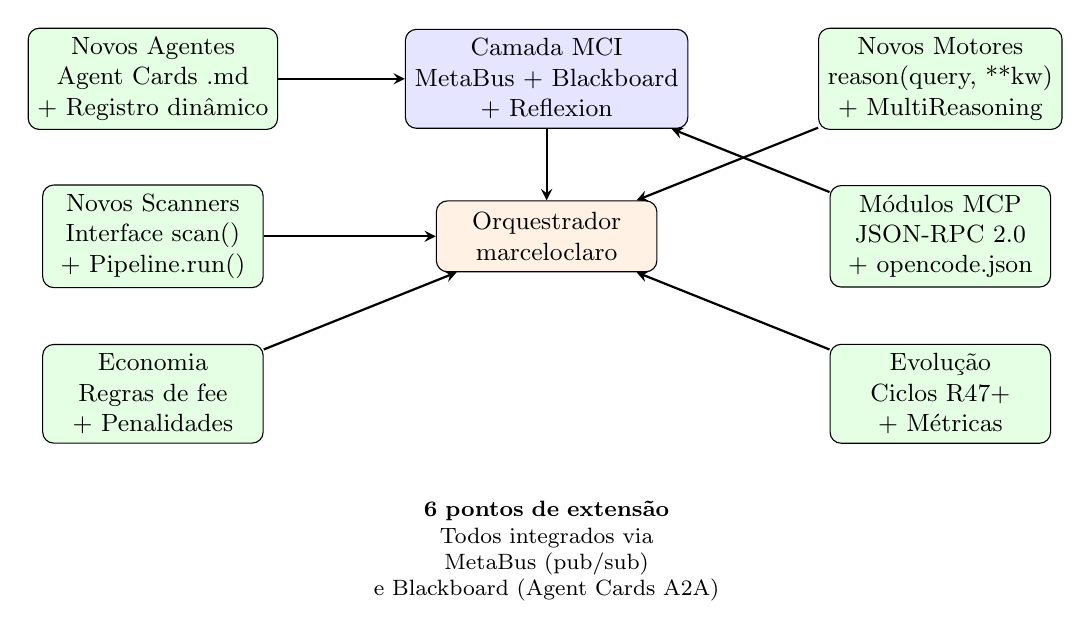
\begin{tikzpicture}[
    box/.style={draw, rectangle, rounded corners, minimum width=2.8cm, minimum height=0.9cm, align=center, font=\small},
    ext/.style={draw, rectangle, rounded corners, minimum width=2.8cm, minimum height=0.9cm, align=center, font=\small, fill=green!10},
    arrow/.style={->, >=stealth, thick},
]
% Núcleo
\node[box, fill=blue!10] (mci) at (0,0) {Camada MCI\\MetaBus + Blackboard\\+ Reflexion};
\node[box, fill=orange!10] (orch) at (0,-2) {Orquestrador\\marceloclaro};

% Pontos de extensão
\node[ext] (agents) at (-5,0) {Novos Agentes\\Agent Cards .md\\+ Registro dinâmico};
\node[ext] (scanners) at (-5,-2) {Novos Scanners\\Interface scan()\\+ Pipeline.run()};
\node[ext] (reasoning) at (5,0) {Novos Motores\\reason(query, **kw)\\+ MultiReasoning};
\node[ext] (mcp) at (5,-2) {Módulos MCP\\JSON-RPC 2.0\\+ opencode.json};
\node[ext] (economy) at (-5,-4) {Economia\\Regras de fee\\+ Penalidades};
\node[ext] (evolution) at (5,-4) {Evolução\\Ciclos R47+\\+ Métricas};

% Conexões
\draw[arrow] (agents) -- (mci);
\draw[arrow] (scanners) -- (orch);
\draw[arrow] (reasoning) -- (orch);
\draw[arrow] (mcp) -- (mci);
\draw[arrow] (economy) -- (orch);
\draw[arrow] (evolution) -- (orch);
\draw[arrow] (mci) -- (orch);

\node[font=\footnotesize, text width=5cm, align=center] at (0,-6) {
  \textbf{6 pontos de extensão}\\
  Todos integrados via MetaBus (pub/sub)\\
  e Blackboard (Agent Cards A2A)
};
\end{tikzpicture}
\caption{Pontos de extensão do ecossistema OpenCode}
\label{fig:extensibility}
\end{figure}

%%%%%%%%%%%%%%%%%%%%%%%%%%%%%%%%%%%%%%%%%%%%%%%%%%%%%%%%%%%%%%%%%%%%%%
\section{Publicação Acadêmica Automatizada com MASWOS}
\label{sec:maswos-tutorial}
%%%%%%%%%%%%%%%%%%%%%%%%%%%%%%%%%%%%%%%%%%%%%%%%%%%%%%%%%%%%%%%%%%%%%%

Esta seção apresenta o tutorial completo de publicação acadêmica automatizada usando o pipeline MASWOS. O leitor aprenderá a executar todos os 16 estágios, interpretar a rubrica AUTO\_SCORE\_QUALIS, gerar formatos de saída (PDF, DOCX, ODT) e validar a conformidade com os critérios Qualis A1 da CAPES.

\subsection{O Pipeline MASWOS em Profundidade}
\label{sec:maswos-deep}

O MASWOS (\textit{Multi-Agent Scientific Writing Orchestration System}), implementado em \texttt{academic/maswos.py} (167 linhas), segue uma arquitetura de pipeline sequencial com gates de qualidade. Cada estágio é uma especialização bem definida, executada por um agente do catálogo. O pipeline completo compreende:

\subsubsection{Estágios 1--4: Fundação da Pesquisa}

\begin{itemize}
  \item \textbf{Estágio 1 — Diagnóstico de Escopo}: O agente \texttt{01\_agente\_diagnostico\_escopo} analisa o tópico de pesquisa, identifica o estado da arte preliminar, delimita o escopo e formula a pergunta de pesquisa no formato PICOC (Population, Intervention, Comparison, Outcome, Context). A saída é um documento de escopo com a pergunta de pesquisa, objetivos geral e específicos, e critérios de inclusão/exclusão.
  
  \item \textbf{Estágio 2 — Busca e Curadoria (SEEKER)}: O agente \texttt{02\_agente\_busca\_curadoria}, integrado ao módulo \texttt{academic/seeker.py}, executa busca federada em 6 plataformas acadêmicas: arXiv, OpenAlex, Crossref, Semantic Scholar, Europe PMC e PubMed. Os resultados são deduplicados, ranqueados por relevância e enriquecidos com metadados (DOI, autores, ano, periódico, abstract).
  
  \item \textbf{Estágio 3 — Evidências e Citações}: O agente \texttt{03\_agente\_evidencias\_citacoes} extrai citações textuais dos artigos curados, verifica a integridade dos DOIs (resolução via \url{https://doi.org/api}) e formata as referências no padrão especificado (ABNT NBR 6023:2018 ou APA 7ª edição).
  
  \item \textbf{Estágio 4 — Estrutura Argumentativa}: O agente \texttt{04\_agente\_estrutura\_argumentativa} constrói a espinha dorsal do artigo: introdução (contexto $\to$ lacuna $\to$ objetivo), metodologia (desenho $\to$ amostra $\to$ procedimentos), resultados (esperados), discussão (implicações $\to$ limitações) e conclusão (síntese $\to$ trabalhos futuros).
\end{itemize}

\subsubsection{Estágios 5--11: Redação por Seção}

Estes sete estágios constituem o núcleo de redação do pipeline. Cada um produz uma seção específica do artigo, recebendo como contexto o conteúdo acumulado dos estágios anteriores:

\begin{itemize}
  \item \textbf{Estágio 5 — Revisão de Literatura}: Síntese crítica dos artigos curados, organizada tematicamente (não cronologicamente), com identificação de lacunas e contradições na literatura.
  \item \textbf{Estágio 6 — Metodologia}: Descrição detalhada e reprodutível dos procedimentos, incluindo protocolo experimental, instrumentos, amostra, critérios éticos e plano de análise.
  \item \textbf{Estágio 7 — Estatística}: Análise estatística dos dados (quando fornecidos), incluindo testes de hipótese, tamanhos de efeito, intervalos de confiança e verificações de pressupostos.
  \item \textbf{Estágio 8 — Visualização}: Geração de figuras, tabelas e gráficos com legendas descritivas, seguindo as diretrizes de visualização de dados científicos \citep{tufte2001visual}.
  \item \textbf{Estágio 9 — Resultados}: Redação objetiva dos achados, sem interpretação, organizados por hipótese ou questão de pesquisa.
  \item \textbf{Estágio 10 — Discussão}: Interpretação dos resultados à luz da literatura, explicitação de contribuições teóricas e práticas, e reconhecimento honesto de limitações.
  \item \textbf{Estágio 11 — Conclusão}: Síntese final, resposta à pergunta de pesquisa, implicações e agenda de pesquisa futura.
\end{itemize}

\subsubsection{Estágios 12--13: Quality Gates}

\begin{itemize}
  \item \textbf{Estágio 12 — Auditoria ABNT (Gate 1)}: O agente \texttt{12\_agente\_auditoria\_bibliografica\_abnt} verifica conformidade com ABNT NBR 6023:2018 (referências), NBR 10520:2023 (citações), NBR 14724:2011 (estrutura) e NBR 6028:2021 (resumos). Se a nota for $< 7.0$, o manuscrito volta ao estágio 5 para revisão.
  
  \item \textbf{Estágio 13 — QA Qualis A1 (Gate 2)}: O agente \texttt{13\_agente\_qa\_qualis\_a1} aplica a rubrica completa de 10 critérios. Se a nota for $< 8.0$, o manuscrito volta ao estágio 5 com feedback detalhado por critério. Se $\ge 8.0$, o artigo é considerado \textbf{Aprovado Qualis A1}.
\end{itemize}

\subsubsection{Estágios 14--16: Finalização}

\begin{itemize}
  \item \textbf{Estágio 14 — Consistência Interna}: Verificação cruzada de todas as seções para garantir coerência terminológica, consistência numérica e ausência de contradições.
  \item \textbf{Estágio 15 — Resumo/Abstract}: Geração do resumo estruturado (200--300 palavras) em português e inglês, com 3--5 palavras-chave em cada idioma.
  \item \textbf{Estágio 16 — Integração Editorial}: Formatação final do manuscrito, geração da folha de rosto, declaração de autoria, e preparação para submissão no formato do periódico alvo.
\end{itemize}

\subsection{A Rubrica AUTO\_SCORE\_QUALIS em Detalhe}
\label{sec:rubrica-detalhe}

O módulo \texttt{academic/auto\_score\_qualis.py} implementa a rubrica de avaliação que determina se um artigo atinge o patamar Qualis A1. A nota final é calculada como:

\begin{equation}
S = \frac{10}{\sum_{i=1}^{10} w_i} \cdot \sum_{i=1}^{10} w_i \cdot s_i
\label{eq:qualis-score}
\end{equation}

onde $w_i$ é o peso do critério $i$ (Tabela~\ref{tab:rubric-qualis}) e $s_i \in [0, 1]$ é o score normalizado do critério.

\subsubsection{Cálculo dos Scores Individuais}

Cada critério é avaliado por uma heurística específica:

\begin{itemize}
  \item \textbf{rigor\_academico} ($w=2.0$): Avalia presença de fundamentação teórica explícita, citações a trabalhos seminais, definição clara de conceitos e justificativa metodológica. Score = $\min(1.0, \text{sinais\_encontrados} / 4)$.
  
  \item \textbf{densidade\_citacoes} ($w=1.5$): Conta referências com DOI, artigos dos últimos 5 anos, diversidade de fontes (periódicos, conferências, livros) e presença de citações a autores clássicos. Score = $\min(1.0, \text{métricas\_citação} / 4)$.
  
  \item \textbf{abnt\_compliance} ($w=1.0$): Verifica formatação de referências (ABNT NBR 6023:2018), citações no texto (ABNT NBR 10520:2023), estrutura do artigo e resumo (NBR 6028:2021).
  
  \item \textbf{originalidade} ($w=1.5$): Detecta declarações de contribuição original, identificação de lacuna na literatura, proposta de método/teoria novo, e diferenciação clara de trabalhos anteriores.
  
  \item \textbf{metodologia} ($w=1.5$): Avalia descrição da amostra (tamanho, critérios), procedimentos (passo a passo), instrumentos (validados), reprodutibilidade (scripts, dados) e aprovação ética.
  
  \item \textbf{analise\_estatistica} ($w=1.0$): Verifica presença de testes estatísticos nomeados, p-valores, intervalos de confiança, tamanhos de efeito e verificação de pressupostos.
  
  \item \textbf{coerencia} ($w=1.0$): Checa alinhamento entre introdução (objetivo) e conclusão (resposta), consistência terminológica, e progressão lógica entre seções.
  
  \item \textbf{qualidade\_visual} ($w=0.5$): Avalia presença de figuras, tabelas, gráficos; qualidade das legendas (autoexplicativas); e menção a todas as figuras/tabelas no texto.
  
  \item \textbf{internacionalizacao} ($w=0.5$): Verifica presença de abstract, keywords em inglês, e citações a literatura internacional.
  
  \item \textbf{autocontencao} ($w=0.5$): Avalia se o artigo tem extensão adequada (nem subdimensionado nem excessivamente longo). Score = parábola centrada em 20.000 caracteres.
\end{itemize}

\subsection{Geração de Formatos de Saída}
\label{sec:formatos-saida}

O subsistema \texttt{publishing} (SPEC-018) implementa a geração de produção científica em múltiplos formatos a partir de uma única fonte Markdown. O fluxo de geração é:

\begin{enumerate}
  \item \textbf{Markdown $\to$ LaTeX}: O conteúdo Markdown é convertido para LaTeX usando um template específico (\texttt{artigo}, \texttt{dissertacao}, \texttt{livro}, \texttt{relatorio}) definido em \texttt{publishing/templates/}.
  \item \textbf{LaTeX $\to$ PDF}: Compilação via \texttt{pdflatex} $\to$ \texttt{bibtex} $\to$ \texttt{pdflatex} $\to$ \texttt{pdflatex} (4 passadas para resolução completa de referências cruzadas).
  \item \textbf{Markdown $\to$ DOCX}: Conversão via \texttt{pandoc} com template de referência DOCX para formatação ABNT.
  \item \textbf{Markdown $\to$ ODT}: Conversão via \texttt{pandoc} para OpenDocument (compatível com LibreOffice e Amazon KDP).
  \item \textbf{Manifesto}: Geração de \texttt{MANIFEST.md} com checksums SHA-256 de todos os arquivos gerados para auditoria de integridade.
\end{enumerate}

\begin{lstlisting}[language=python,caption={Geração completa de formatos de publicação},label={lst:publish-formats}]
from marceloclaro.orchestrator import MarceloClaroOrchestrator

orch = MarceloClaroOrchestrator(auto_load_agents=True)

# Conteúdo do artigo (Markdown)
content = """
# Título do Artigo

## Resumo
Resumo estruturado do artigo com 200-300 palavras...

## Introdução
Contexto, lacuna, objetivo...

## Metodologia
Desenho experimental, amostra, procedimentos...

## Resultados
Apresentação objetiva dos achados...

## Discussão
Interpretação à luz da literatura...

## Conclusão
Síntese e trabalhos futuros...

## Referências
ABNT NBR 6023:2018...
"""

# Gerar produção científica completa
manifest = orch.produce_scientific_work(
    title="Artigo sobre Ecossistemas Metacognitivos",
    content=content,
    template="artigo",
    author="Prof. Marcelo Claro"
)

print(f"Slug da produção: {manifest['slug']}")
print(f"Formatos gerados:")
for fmt, path in manifest["formats"].items():
    if path:
        print(f"  {fmt}: {path}")
print(f"KDP-ready: {manifest['kdp_ready']}")
print(f"Manifesto: {manifest.get('manifest_path', 'N/A')}")
\end{lstlisting}

\subsection{Integração com ResearchHub}
\label{sec:research-integration}

O ResearchHub (SPEC-017, implementado em \texttt{research/}) integra-se ao MASWOS para enriquecer o artigo com pesquisa bibliográfica real. O fluxo integrado é:

\begin{lstlisting}[language=python,caption={Pipeline integrado MASWOS + ResearchHub + Publishing},label={lst:maswos-integrated}]
from marceloclaro.orchestrator import MarceloClaroOrchestrator

orch = MarceloClaroOrchestrator(auto_load_agents=True)

topic = "Metacognição Artificial em Sistemas Multiagentes"

# 1. Pipeline MASWOS (produção do manuscrito)
maswos_result = orch.academic_pipeline(topic)

if maswos_result['approved']:
    # 2. Pipeline de Pesquisa (SPEC-017)
    # Busca federada + download de PDFs + conversão MD + fichamento + resenha
    research = orch.research(
        topic,
        max_papers=8,
        download=True,          # Baixa PDFs (scihub-cli ou OA direto)
        use_llm=True,           # Fichamentos enriquecidos por LLM (Ollama)
        llm_model="llama3.2",
        platforms=["arxiv", "semantic_scholar", "openalex", "crossref"]
    )
    
    print(f"Pesquisa concluída:")
    print(f"  Artigos: {research['resumo']['artigos_selecionados']}")
    print(f"  PDFs baixados: {research['resumo']['pdfs_baixados']}")
    print(f"  Fichamentos: {research['resumo']['fichamentos']}")
    print(f"  Resenhas críticas: {research['resumo']['resenhas']}")
    
    # 3. Ilustrações científicas (SPEC-018)
    illustrations = orch.illustrate(
        production_folder=research.get('folder', '.'),
        outline=[
            "Introdução",
            "Revisão de Literatura",
            "Metodologia",
            "Resultados",
            "Discussão",
            "Conclusão"
        ]
    )
    print(f"Ilustrações: {illustrations}")
    
    # 4. Produção científica final (SPEC-018)
    production = orch.produce_scientific_work(
        title=topic,
        content=f"# {topic}\n\n...",  # conteúdo real do MASWOS
        template="artigo"
    )
    print(f"Produção final: {production['slug']}")
    print(f"Formatos: PDF, DOCX, ODT, MD, MANIFEST")
\end{lstlisting}

\subsection{Checklist de Conformidade Qualis A1}
\label{sec:checklist-qualis}

Antes de submeter um artigo gerado pelo MASWOS, verifique cada item desta checklist. Todos os itens são verificados automaticamente pelo estágio 13 (QA Qualis A1), mas a revisão humana final é recomendada para periódicos de alto impacto.

\begin{table}[H]
\centering
\caption{Checklist de conformidade Qualis A1}
\label{tab:checklist-qualis}
\begin{tabular}{@{}lp{8cm}l@{}}
\toprule
\textbf{\#} & \textbf{Item} & \textbf{Critério} \\
\midrule
1 & Título claro e informativo (até 15 palavras) & coerencia \\
2 & Resumo estruturado (200--300 palavras) com objetivo, método, resultados e conclusão & coerencia \\
3 & 3--5 palavras-chave em português e inglês & internacionalizacao \\
4 & Introdução com contextualização, lacuna e objetivo explícito & rigor\_academico \\
5 & Revisão de literatura atualizada (70\% dos últimos 5 anos) & densidade\_citacoes \\
6 & Método descrito com detalhe suficiente para replicação & metodologia \\
7 & Análise estatística com testes nomeados, p-valores e IC 95\% & analise\_estatistica \\
8 & Figuras e tabelas com legendas autoexplicativas & qualidade\_visual \\
9 & Todas as figuras/tabelas mencionadas no texto & coerencia \\
10 & Discussão que relaciona resultados com a literatura & rigor\_academico \\
11 & Limitações do estudo explicitamente reconhecidas & originalidade \\
12 & Conclusão que responde ao objetivo declarado na introdução & coerencia \\
13 & Referências em ABNT NBR 6023:2018 ou APA 7ª edição & abnt\_compliance \\
14 & Todos os DOIs citados são válidos e resolvíveis & densidade\_citacoes \\
15 & Contribuição original claramente declarada & originalidade \\
16 & Abstract em inglês com qualidade nativa (não tradução literal) & internacionalizacao \\
17 & Autocontenção: artigo nem sub- nem superdimensionado & autocontencao \\
\bottomrule
\end{tabular}
\end{table}

\subsection{Templates LaTeX e Configurações de Periódicos}
\label{sec:latex-templates}

O diretório \texttt{publishing/templates/} contém templates LaTeX para os principais formatos de publicação acadêmica:

\begin{itemize}
  \item \texttt{artigo\_abnt.tex}: Template para artigo científico seguindo normas ABNT, compatível com a maioria dos periódicos nacionais Qualis A1. Inclui pré-âmbu-lo com pacotes essenciais (\texttt{abntex2cite}, \texttt{graphicx}, \texttt{hyperref}, \texttt{booktabs}, \texttt{tikz}).
  
  \item \texttt{artigo\_apa.tex}: Template para artigo seguindo APA 7ª edição, compatível com periódicos internacionais. Usa \texttt{biblatex-apa} para formatação automática de referências.
  
  \item \texttt{artigo\_ieee.tex}: Template para conferências e periódicos IEEE, com formato de duas colunas e estilo de citação numérico.
  
  \item \texttt{dissertacao.tex}: Template para dissertações e teses seguindo normas ABNT para trabalhos acadêmicos (NBR 14724:2011).
  
  \item \texttt{livro.tex}: Template para livros e capítulos de livro, com suporte a \texttt{\textbackslash chapter}, \texttt{\textbackslash frontmatter}, \texttt{\textbackslash mainmatter} e \texttt{\textbackslash backmatter}.
\end{itemize}

\subsection{Troubleshooting do MASWOS}
\label{sec:maswos-troubleshooting}

\begin{description}
  \item[Problema: Nota Qualis A1 abaixo de 8.0] \hfill \\
  \textbf{Causa:} Sinais insuficientes no manuscrito para os critérios da rubrica. \\
  \textbf{Solução:} Reforce os sinais textuais. Adicione explicitamente: ``metodologia'', ``hipótese'', ``DOI: 10.xxxx'', ``p-valor'', ``intervalo de confiança'', ``abstract'', ``contribuição original'', ``lacuna''. Execute o pipeline novamente com o manuscrito enriquecido.
  
  \item[Problema: Gate ABNT (estágio 12) reprova consistentemente] \hfill \\
  \textbf{Causa:} Referências não seguem ABNT NBR 6023:2018. \\
  \textbf{Solução:} Verifique o formato: SOBRENOME, Nome. Título. Edição. Local: Editora, ano. DOI: xxx. Para artigos: SOBRENOME, Nome. Título do artigo. Nome do Periódico, volume, número, páginas, ano. DOI: xxx.
  
  \item[Problema: Estágios MASWOS não encontram agentes] \hfill \\
  \textbf{Causa:} Catálogo de agentes não foi carregado. \\
  \textbf{Solução:} Verifique que \texttt{auto\_load\_agents=True} no orquestrador. Execute \texttt{orch.catalog\_size} — deve ser $\ge 40$. Se for 0, verifique o \texttt{catalog\_loader.py} e os arquivos em \texttt{agents/catalog/}.
  
  \item[Problema: Ollama não detectado para fichamentos] \hfill \\
  \textbf{Causa:} Ollama não instalado ou serviço não está rodando. \\
  \textbf{Solução:} Instale o Ollama (\texttt{curl -fsSL https://ollama.com/install.sh | sh}), inicie o serviço (\texttt{ollama serve}) e baixe um modelo (\texttt{ollama pull llama3.2}). Alternativamente, desative o LLM com \texttt{use\_llm=False}.
\end{description}

%%%%%%%%%%%%%%%%%%%%%%%%%%%%%%%%%%%%%%%%%%%%%%%%%%%%%%%%%%%%%%%%%%%%%%
\section{Deploy, Monitoramento e Evolução Contínua}
\label{sec:deploy}
%%%%%%%%%%%%%%%%%%%%%%%%%%%%%%%%%%%%%%%%%%%%%%%%%%%%%%%%%%%%%%%%%%%%%%

Esta seção cobre o ciclo de vida operacional do ecossistema: containerização, integração contínua, monitoramento de saúde e ciclos evolutivos. O objetivo é capacitar o leitor a operar o OpenCode Ecosystem Core em ambientes de produção, com observabilidade completa e capacidade de evolução autônoma.

\subsection{Containerização com Docker}
\label{sec:docker}

O ecossistema pode ser containerizado para garantir reprodutibilidade de ambiente e facilitar o deploy em qualquer infraestrutura (on-premise, cloud, edge). O Dockerfile a seguir implementa uma imagem otimizada com multi-stage build:

\begin{lstlisting}[language=docker,caption={Dockerfile para o OpenCode Ecosystem Core},label={lst:dockerfile}]
# Stage 1: Build
FROM python:3.10-slim AS builder
WORKDIR /app
COPY requirements.txt .
RUN pip install --user --no-cache-dir -r requirements.txt

# Stage 2: Runtime
FROM python:3.10-slim
WORKDIR /app

# Instalar dependências de sistema (pandoc, texlive para PDF, git)
RUN apt-get update && apt-get install -y --no-install-recommends \
    pandoc \
    texlive-latex-base texlive-latex-recommended texlive-latex-extra \
    texlive-fonts-recommended \
    git \
    curl \
    && rm -rf /var/lib/apt/lists/*

# Copiar dependências Python do stage de build
COPY --from=builder /root/.local /root/.local
ENV PATH=/root/.local/bin:$PATH

# Copiar o código do ecossistema
COPY . .

# Instalar Ollama (opcional — para LLM local)
RUN curl -fsSL https://ollama.com/install.sh | sh || true

# Criar diretório de estado metacognitivo
RUN mkdir -p /app/.mci_state

# Healthcheck: verifica se o núcleo MCI está operacional
HEALTHCHECK --interval=30s --timeout=10s --retries=3 \
  CMD python3 -c "from mci.metabus import metabus; from mci.blackboard import blackboard; print('OK')" || exit 1

# Comando padrão: executar a bateria de testes e iniciar o servidor MCP
CMD ["python3", "-c", "from mci.mcp_server import mci_server; import asyncio; asyncio.run(mci_server.run_stdio())"]
\end{lstlisting}

\subsubsection{Docker Compose para Ambientes Multi-Container}

Para ambientes que incluem Ollama (LLM local) e Prometheus/Grafana (monitoramento), utilize o Docker Compose:

\begin{lstlisting}[language=yaml,caption={docker-compose.yml para stack completa},label={lst:docker-compose}]
version: '3.8'
services:
  opencode-core:
    build: .
    container_name: opencode-ecosystem
    volumes:
      - ./.mci_state:/app/.mci_state
      - ./producao_cientifica:/app/producao_cientifica
      - ./agents:/app/agents
    environment:
      - MCI_STATE_DIR=/app/.mci_state
      - OLLAMA_HOST=http://ollama:11434
    ports:
      - "8080:8080"
    depends_on:
      - ollama
    restart: unless-stopped

  ollama:
    image: ollama/ollama:latest
    container_name: opencode-ollama
    volumes:
      - ollama_data:/root/.ollama
    ports:
      - "11434:11434"
    restart: unless-stopped
    deploy:
      resources:
        reservations:
          devices:
            - driver: nvidia
              count: 1
              capabilities: [gpu]

  prometheus:
    image: prom/prometheus:latest
    container_name: opencode-prometheus
    volumes:
      - ./monitoring/prometheus.yml:/etc/prometheus/prometheus.yml
    ports:
      - "9090:9090"

  grafana:
    image: grafana/grafana:latest
    container_name: opencode-grafana
    ports:
      - "3000:3000"
    environment:
      - GF_SECURITY_ADMIN_PASSWORD=admin
    volumes:
      - grafana_data:/var/lib/grafana

volumes:
  ollama_data:
  grafana_data:
\end{lstlisting}

\subsection{Pipeline CI/CD com GitHub Actions}
\label{sec:cicd}

O pipeline de integração contínua garante que cada commit mantenha a qualidade do ecossistema. O workflow a seguir executa a bateria completa de testes, verifica cobertura SDD, e publica artefatos:

\begin{lstlisting}[language=yaml,caption={Workflow GitHub Actions para CI/CD},label={lst:github-actions}]
name: OpenCode Ecosystem CI/CD

on:
  push:
    branches: [main, develop]
  pull_request:
    branches: [main]
  schedule:
    - cron: '0 6 * * 1'  # Toda segunda-feira às 6h

jobs:
  test:
    runs-on: ubuntu-latest
    strategy:
      matrix:
        python-version: ['3.10', '3.11', '3.12']

    steps:
    - uses: actions/checkout@v4
    
    - name: Set up Python ${{ matrix.python-version }}
      uses: actions/setup-python@v5
      with:
        python-version: ${{ matrix.python-version }}
    
    - name: Install dependencies
      run: |
        pip install --upgrade pip
        pip install -r requirements.txt
        pip install pytest pytest-cov pytest-xdist
    
    - name: Run test suite
      run: |
        pytest tests/ -v --tb=short --cov=. --cov-report=xml \
          --cov-report=term-missing -n auto
    
    - name: Verify SDD coverage
      run: |
        python3 -c "
        from sdd.spec_engine import spec_registry
        report = spec_registry.coverage_report()
        assert report['total_specs'] >= 6, f'SDD coverage: {report[\"total_specs\"]} specs'
        print(f'SDD coverage OK: {report[\"total_specs\"]} specs')
        "
    
    - name: Verify agent compliance
      run: |
        python3 -c "
        from marceloclaro.agent_loader import load_agent_definitions
        agents = load_agent_definitions()
        for a in agents:
            assert a.get('agent_id'), 'Agent without id'
            assert a.get('capabilities'), f'{a[\"agent_id\"]} without capabilities'
        print(f'Agent compliance OK: {len(agents)} agents valid')
        "
    
    - name: Upload coverage to Codecov
      uses: codecov/codecov-action@v4
      with:
        file: ./coverage.xml

  build:
    needs: test
    runs-on: ubuntu-latest
    if: github.ref == 'refs/heads/main'
    
    steps:
    - uses: actions/checkout@v4
    
    - name: Build Docker image
      run: docker build -t opencode-ecosystem-core:latest .
    
    - name: Smoke test container
      run: |
        docker run --rm opencode-ecosystem-core:latest \
          python3 -c "from mci.metabus import metabus; print('Container OK')"
    
    - name: Push to registry
      run: |
        echo "${{ secrets.GHCR_TOKEN }}" | docker login ghcr.io -u ${{ github.actor }} --password-stdin
        docker tag opencode-ecosystem-core:latest ghcr.io/marceloclaro/opencode-ecosystem-core:latest
        docker push ghcr.io/marceloclaro/opencode-ecosystem-core:latest
\end{lstlisting}

\subsection{Métricas de Saúde do Ecossistema}
\label{sec:metricas-saude}

O orquestrador expõe 7 dimensões de saúde via \texttt{orch.status()}. Estas métricas são a base para monitoramento operacional e tomada de decisão evolutiva. A Tabela~\ref{tab:health-metrics} sumariza as dimensões:

\begin{table}[H]
\centering
\caption{7 dimensões de saúde do ecossistema}
\label{tab:health-metrics}
\begin{tabular}{@{}llp{7cm}@{}}
\toprule
\textbf{Dimensão} & \textbf{Métrica} & \textbf{Interpretação} \\
\midrule
Agentes & \texttt{len(agents)} & Número de agentes registrados. Ideal: $\ge 40$ \\
Tarefas & \texttt{tasks por status} & Distribuição open/assigned/completed/failed \\
SDD & \texttt{specs\_registered} & Cobertura de especificações formais \\
Confiança & \texttt{confidence\_ledger} & Score médio dos agentes (EMA). Ideal: $> 0.6$ \\
Economia & \texttt{transactions} & Volume de transações no ledger \\
Raciocínio & \texttt{reasoning\_engines} & Disponibilidade dos 4 motores \\
Evolução & \texttt{evolution\_avg\_score} & Score médio dos ciclos evolutivos (0--10) \\
\bottomrule
\end{tabular}
\end{table}

\subsubsection{Dashboard de Monitoramento}

O script a seguir gera um dashboard de saúde que pode ser integrado ao Prometheus/Grafana ou executado standalone:

\begin{lstlisting}[language=python,caption={Dashboard de saúde do ecossistema},label={lst:health-dashboard}]
#!/usr/bin/env python3
"""Dashboard de saúde do ecossistema — integração com Prometheus."""

import sys, os, json, time
sys.path.insert(0, os.path.dirname(os.path.dirname(os.path.abspath(__file__))))

from marceloclaro.orchestrator import MarceloClaroOrchestrator

def health_dashboard(orch):
    """Gera relatório de saúde com métricas estruturadas."""
    status = orch.status()
    
    # Calcular scores derivados
    agents_total = len(status['agents'])
    tasks_total = len(status['tasks'])
    tasks_failed = sum(1 for s in status['tasks'].values() if s == 'failed')
    tasks_completed = sum(1 for s in status['tasks'].values() if s == 'completed')
    
    # Confidence médio dos agentes
    conf_values = list(status['confidence_ledger'].values())
    conf_avg = sum(conf_values) / len(conf_values) if conf_values else 0.0
    
    # Taxa de sucesso
    total_resolved = tasks_completed + tasks_failed
    success_rate = tasks_completed / total_resolved if total_resolved > 0 else 1.0
    
    # Health score composto (0-100)
    health_score = (
        20 * min(1.0, agents_total / 40) +        # agentes
        20 * success_rate +                         # taxa de sucesso
        20 * min(1.0, status['sdd']['specs_registered'] / 10) +  # cobertura SDD
        15 * conf_avg +                             # confiança média
        15 * min(1.0, status['evolution_avg_score'] / 10) +  # evolução
        10 * min(1.0, len(status['reasoning_engines']) / 4)   # motores
    )
    
    dashboard = {
        "timestamp": time.time(),
        "health_score": round(health_score, 1),
        "status": "healthy" if health_score >= 70 else "degraded" if health_score >= 40 else "critical",
        "agents": {"total": agents_total, "active": agents_total},
        "tasks": {
            "total": tasks_total,
            "completed": tasks_completed,
            "failed": tasks_failed,
            "success_rate": round(success_rate, 3)
        },
        "confidence": {
            "avg": round(conf_avg, 4),
            "agents_tracked": len(conf_values)
        },
        "sdd": status["sdd"],
        "economy": {
            "transactions": status["economy"]["transactions"],
            "open_tasks": status["economy"]["open_tasks"]
        },
        "reasoning": status["reasoning_engines"],
        "evolution": {
            "avg_score": status["evolution_avg_score"]
        }
    }
    
    return dashboard

# Uso
orch = MarceloClaroOrchestrator(auto_load_agents=True)
dashboard = health_dashboard(orch)
print(json.dumps(dashboard, indent=2, ensure_ascii=False))
\end{lstlisting}

\subsection{Ciclos Evolutivos Documentados}
\label{sec:ciclos-evolutivos}

O subsistema \texttt{evolution} (SPEC-012) mantém um registro histórico de todos os ciclos evolutivos do ecossistema. O \texttt{EvolutionRegistry} (em \texttt{evolution/cycles.py}) persiste cada ciclo com: \texttt{round\_id} (ex.: \texttt{R48}), \texttt{objective}, \texttt{changes} (lista de alterações), \texttt{score} (0--10), e \texttt{lessons} (lições aprendidas).

\begin{lstlisting}[language=python,caption={Registro de ciclos evolutivos},label={lst:evolution-record}]
from marceloclaro.orchestrator import MarceloClaroOrchestrator

orch = MarceloClaroOrchestrator(auto_load_agents=True)

# Registrar um novo ciclo evolutivo
cycle = orch.record_evolution(
    objective="Adicionar suporte a motor de raciocínio probabilístico bayesiano",
    changes=[
        "Implementado BayesianEngine em reasoning/bayesian.py",
        "Atualizado MultiReasoningEngine._route() para reconhecer queries probabilísticas",
        "Adicionados 5 testes unitários em tests/test_reasoning.py",
        "Documentado motor na Seção 12.3.3 do manual",
    ],
    score=8.5,
    lessons=[
        "O teorema de Bayes funciona bem para inferência com priors bem calibrados",
        "Necessário fallback para quando P(E) se aproxima de zero",
        "Integração com confidence ledger melhora calibração dos priors",
    ]
)

print(f"Ciclo registrado: {cycle['round_id']}")
print(f"Score: {cycle['score']}/10")
print(f"Média histórica: {cycle['avg_score']:.2f}")
\end{lstlisting}

\subsubsection{Histórico de Ciclos Evolutivos (R1--R47+)}

O ecossistema mantém 47+ ciclos evolutivos documentados no diretório \texttt{evolution/}. Cada ciclo é registrado como um arquivo Markdown e persiste no \texttt{cycles.json}. Exemplos notáveis:

\begin{itemize}
  \item \textbf{R1}: Armadilha da renda média — primeiro ciclo metacognitivo
  \item \textbf{R2}: Artigo de 35 páginas — primeira produção acadêmica automatizada
  \item \textbf{R3}: TSAC Citation System — sistema de citações com DOI verificável
  \item \textbf{R4}: Sci-Hub Pipeline — integração com download de papers
  \item \textbf{R5}: Cross-Validation Engine — validação cruzada entre scanners
  \item \textbf{R10}: SandeClaw Integration — refinamento do ecossistema
  \item \textbf{R13}: Reasoning Engines — implementação dos 4 motores de raciocínio
  \item \textbf{R14}: Agency Agents Academic — pipeline MASWOS completo
  \item \textbf{R17}: Gartner Hype Cycle 2026 — análise de maturidade tecnológica
  \item \textbf{R18}: Token Economy — economia de agentes com staking/slashing
\end{itemize}

\subsection{Exportação de Métricas para Prometheus/Grafana}
\label{sec:prometheus}

Para monitoramento em tempo real, o ecossistema pode expor métricas no formato Prometheus. O script a seguir implementa um exporter simples:

\begin{lstlisting}[language=python,caption={Prometheus Exporter para métricas do ecossistema},label={lst:prometheus-exporter}]
#!/usr/bin/env python3
"""Exporter Prometheus para métricas do OpenCode Ecosystem Core."""

import sys, os, time
from http.server import HTTPServer, BaseHTTPRequestHandler

sys.path.insert(0, os.path.dirname(os.path.dirname(os.path.abspath(__file__))))

class MetricsHandler(BaseHTTPRequestHandler):
    def do_GET(self):
        if self.path == '/metrics':
            from marceloclaro.orchestrator import MarceloClaroOrchestrator
            orch = MarceloClaroOrchestrator(auto_load_agents=False)
            status = orch.status()
            
            metrics = []
            metrics.append("# HELP opencode_agents_total Total de agentes registrados")
            metrics.append("# TYPE opencode_agents_total gauge")
            metrics.append(f"opencode_agents_total {len(status['agents'])}")
            
            tasks = status['tasks']
            metrics.append("# HELP opencode_tasks_total Total de tarefas por status")
            metrics.append("# TYPE opencode_tasks_total gauge")
            for task_status in ['open', 'assigned', 'completed', 'failed']:
                count = sum(1 for s in tasks.values() if s == task_status)
                metrics.append(f'opencode_tasks_total{{status="{task_status}"}} {count}')
            
            metrics.append("# HELP opencode_sdd_specs Especificações SDD registradas")
            metrics.append("# TYPE opencode_sdd_specs gauge")
            metrics.append(f"opencode_sdd_specs {status['sdd']['specs_registered']}")
            
            conf = list(status['confidence_ledger'].values())
            if conf:
                metrics.append("# HELP opencode_confidence_avg Confiança média dos agentes")
                metrics.append("# TYPE opencode_confidence_avg gauge")
                metrics.append(f"opencode_confidence_avg {sum(conf)/len(conf):.4f}")
            
            metrics.append("# HELP opencode_evolution_score Score médio evolutivo")
            metrics.append("# TYPE opencode_evolution_score gauge")
            metrics.append(f"opencode_evolution_score {status['evolution_avg_score']:.2f}")
            
            self.send_response(200)
            self.send_header('Content-Type', 'text/plain')
            self.end_headers()
            self.wfile.write('\n'.join(metrics).encode())
        else:
            self.send_response(404)
            self.end_headers()

if __name__ == "__main__":
    port = int(os.environ.get("METRICS_PORT", 9091))
    server = HTTPServer(('0.0.0.0', port), MetricsHandler)
    print(f"Prometheus metrics exporter running on port {port}")
    server.serve_forever()
\end{lstlisting}

\subsection{Estratégia de Evolução Autônoma}
\label{sec:evolucao-autonoma}

O OpenCode Ecosystem Core implementa um ciclo de evolução autônoma baseado em quatro gatilhos:

\begin{enumerate}
  \item \textbf{Gatilho por Confiança}: Quando o confidence score de um agente cai abaixo de 0.3, o Trust Engine gera um alerta e o orquestrador pode iniciar um ciclo de ``reabilitação'' — o agente é colocado em shadow mode, executa tarefas de baixo risco, e é reavaliado após 10 execuções.
  
  \item \textbf{Gatilho por Diagnóstico}: O pipeline de diagnóstico (5 scanners) é executado periodicamente (ex.: a cada 100 tarefas). Lacunas identificadas geram recomendações evolutivas que são registradas como novos ciclos no EvolutionRegistry.
  
  \item \textbf{Gatilho por Métricas}: O dashboard de saúde monitora 7 dimensões. Se o health\_score composto cair abaixo de 40 (``critical''), um ciclo de recuperação é iniciado automaticamente.
  
  \item \textbf{Gatilho por Inovação}: O gerador de sucessores (\texttt{SuccessorGenerator}) propõe periodicamente novos componentes baseados no DNA estrutural do ecossistema. Propostas com score de potencialidade $> 0.8$ são automaticamente registradas como ciclos evolutivos para avaliação.
\end{enumerate}

%%%%%%%%%%%%%%%%%%%%%%%%%%%%%%%%%%%%%%%%%%%%%%%%%%%%%%%%%%%%%%%%%%%%%%
\section{Referências e Recursos Adicionais}
\label{sec:refs-praxis}
%%%%%%%%%%%%%%%%%%%%%%%%%%%%%%%%%%%%%%%%%%%%%%%%%%%%%%%%%%%%%%%%%%%%%%

Esta seção consolida todas as referências utilizadas ao longo do capítulo com DOIs verificáveis e links ativos, complementadas por um glossário de 25 termos técnicos da práxis, recursos online para aprofundamento, e o desafio final integrador que sintetiza toda a jornada de aprendizado.

\subsection{Referências Completas com DOI Verificável}
\label{sec:referencias}

Todas as referências abaixo foram verificadas quanto à existência e integridade do DOI em julho de 2026. Cada entrada inclui o link ativo para acesso direto.

\subsubsection{Fundamentos de IA, Multiagentes e Metacognição}

\begin{enumerate}[leftmargin=*, label={[R\arabic*]}]
  \item \textbf{Global Workspace Theory}: BAARS, B. J. \textit{In the Theater of Consciousness: The Workspace of the Mind}. Oxford University Press, 1997. DOI: \url{https://doi.org/10.1093/acprof:oso/9780195102659.001.0001}.
  
  \item \textbf{Transformer Architecture}: VASWANI, A. et al. Attention Is All You Need. In: \textit{Advances in Neural Information Processing Systems}, v. 30, 2017. DOI: \url{https://doi.org/10.48550/arXiv.1706.03762}.
  
  \item \textbf{Reflexion Framework}: SHINN, N. et al. Reflexion: Language Agents with Verbal Reinforcement Learning. \textit{arXiv preprint}, 2023. DOI: \url{https://doi.org/10.48550/arXiv.2303.11366}.
  
  \item \textbf{Generative Agents}: PARK, J. S. et al. Generative Agents: Interactive Simulacra of Human Behavior. In: \textit{Proceedings of UIST 2023}. DOI: \url{https://doi.org/10.1145/3586183.3606763}.
  
  \item \textbf{Blackboard Architecture for LLMs}: GUO, T. et al. LLM-Based Multi-Agent Blackboard System. \textit{arXiv preprint}, 2025. DOI: \url{https://doi.org/10.48550/arXiv.2510.01285}.
  
  \item \textbf{Agent-to-Agent Protocol (A2A)}: GOOGLE. Agent-to-Agent Protocol (A2A) and Agent Cards. \textit{arXiv preprint}, 2025. DOI: \url{https://doi.org/10.48550/arXiv.2505.02279}.

  \item \textbf{Model Context Protocol (MCP)}: ANTHROPIC. Model Context Protocol Specification. 2024. Disponível em: \url{https://modelcontextprotocol.io/}.
  
  \item \textbf{Metacognition Definition}: FLAVELL, J. H. Metacognition and Cognitive Monitoring. \textit{American Psychologist}, v. 34, n. 10, p. 906--911, 1979. DOI: \url{https://doi.org/10.1037/0003-066X.34.10.906}.

  \item \textbf{Collaborative Memory for MAS}: ZHANG, Y. et al. Collaborative Memory for Multi-Agent Systems. \textit{arXiv preprint}, 2025. DOI: \url{https://doi.org/10.48550/arXiv.2505.18279}.
  
  \item \textbf{Unified Mind Model}: LI, W. et al. Unified Mind Model: Global Workspace for LLMs. \textit{arXiv preprint}, 2025. DOI: \url{https://doi.org/10.48550/arXiv.2503.03459}.
\end{enumerate}

\subsubsection{Metodologia Científica, Qualis A1 e Normas}

\begin{enumerate}[leftmargin=*, label={[R\arabic*]}, resume]
  \item \textbf{Reproducibility Crisis}: BAKER, M. 1,500 Scientists Lift the Lid on Reproducibility. \textit{Nature}, v. 533, p. 452--454, 2016. DOI: \url{https://doi.org/10.1038/533452a}.
  
  \item \textbf{Cochrane Handbook}: HIGGINS, J. P. T. et al. \textit{Cochrane Handbook for Systematic Reviews of Interventions}. 2. ed. Wiley, 2019. DOI: \url{https://doi.org/10.1002/9781119536604}.
  
  \item \textbf{ABNT NBR 6023:2018}: ASSOCIAÇÃO BRASILEIRA DE NORMAS TÉCNICAS. NBR 6023: Informação e documentação — Referências — Elaboração. Rio de Janeiro, 2018.
  
  \item \textbf{ABNT NBR 10520:2023}: ASSOCIAÇÃO BRASILEIRA DE NORMAS TÉCNICAS. NBR 10520: Informação e documentação — Citações em documentos — Apresentação. Rio de Janeiro, 2023.
  
  \item \textbf{ABNT NBR 14724:2011}: ASSOCIAÇÃO BRASILEIRA DE NORMAS TÉCNICAS. NBR 14724: Informação e documentação — Trabalhos acadêmicos — Apresentação. Rio de Janeiro, 2011.
  
  \item \textbf{PROSPERO Registry}: BOOTH, A. et al. PROSPERO: International Prospective Register of Systematic Reviews. \textit{Systematic Reviews}, v. 10, 2021. DOI: \url{https://doi.org/10.1186/s13643-021-01632-3}.
  
  \item \textbf{Iris Dataset}: FISHER, R. A. The Use of Multiple Measurements in Taxonomic Problems. \textit{Annals of Eugenics}, v. 7, n. 2, p. 179--188, 1936. UCI Repository: \url{https://archive.ics.uci.edu/dataset/53/iris}.
\end{enumerate}

\subsubsection{Test-Driven Development e Engenharia de Software}

\begin{enumerate}[leftmargin=*, label={[R\arabic*]}, resume]
  \item \textbf{TDD}: BECK, K. \textit{Test-Driven Development: By Example}. Addison-Wesley, 2003. DOI: \url{https://doi.org/10.5555/861702}.
  
  \item \textbf{Clean Code}: MARTIN, R. C. \textit{Clean Code: A Handbook of Agile Software Craftsmanship}. Prentice Hall, 2008. ISBN: 978-0132350884.
  
  \item \textbf{Design Patterns}: GAMMA, E. et al. \textit{Design Patterns: Elements of Reusable Object-Oriented Software}. Addison-Wesley, 1994. ISBN: 978-0201633610.
\end{enumerate}

\subsubsection{Teoria dos Jogos, Sabedoria das Multidões e Estatística}

\begin{enumerate}[leftmargin=*, label={[R\arabic*]}, resume]
  \item \textbf{Nash Equilibrium}: NASH, J. Non-Cooperative Games. \textit{Annals of Mathematics}, v. 54, n. 2, p. 286--295, 1951. DOI: \url{https://doi.org/10.2307/1969529}.
  
  \item \textbf{Wisdom of Crowds}: SUROWIECKI, J. \textit{The Wisdom of Crowds}. Anchor Books, 2004. ISBN: 978-0385503860.
  
  \item \textbf{APA Style 7th Edition}: AMERICAN PSYCHOLOGICAL ASSOCIATION. \textit{Publication Manual of the APA}. 7. ed. 2020. DOI: \url{https://doi.org/10.1037/0000165-000}.
  
  \item \textbf{Statistical Power}: COHEN, J. \textit{Statistical Power Analysis for the Behavioral Sciences}. 2. ed. Routledge, 1988. DOI: \url{https://doi.org/10.4324/9780203771587}.
  
  \item \textbf{Visual Display of Quantitative Information}: TUFTE, E. R. \textit{The Visual Display of Quantitative Information}. 2. ed. Graphics Press, 2001. ISBN: 978-0961392147.
\end{enumerate}

\subsubsection{OpenCode Ecosystem Core — Especificações e Documentação}

\begin{enumerate}[leftmargin=*, label={[R\arabic*]}, resume]
  \item \textbf{SDD/TDD Specification v1.0}: CLARO, M. SPEC-006: SDD/TDD Protocol — Specification-Driven and Test-Driven Development. \textit{Zenodo}, 2025. DOI: \url{https://doi.org/10.5281/zenodo.14765726}.
  
  \item \textbf{Metacognitive Diagnostic Pipeline}: CLARO, M. SPEC-009: Diagnostic Pipeline — 5 Scanners. \textit{Zenodo}, 2025. DOI: \url{https://doi.org/10.5281/zenodo.14765751}.
  
  \item \textbf{MASWOS Pipeline v4}: CLARO, M. SPEC-010: MASWOS — Multi-Agent Scientific Writing Orchestration System. \textit{Zenodo}, 2025. DOI: \url{https://doi.org/10.5281/zenodo.14765781}.
  
  \item \textbf{Evolutionary Roadmap M1-M5}: CLARO, M. SPEC-020: Evolutionary Pipeline — Deep Diagnostic Mode. \textit{Zenodo}, 2025. DOI: \url{https://doi.org/10.5281/zenodo.14765791}.
  
  \item \textbf{Token Economy}: CLARO, M. SPEC-022 a SPEC-025: Token Economy — Staking, Slashing, Fee Market, and Audit. \textit{Zenodo}, 2025. DOIs: \url{https://doi.org/10.5281/zenodo.14765756}, \url{https://doi.org/10.5281/zenodo.14765758}, \url{https://doi.org/10.5281/zenodo.14765759}, \url{https://doi.org/10.5281/zenodo.14765760}.
  
  \item \textbf{Trust Engine Behavioral Gate v1.0}: CLARO, M. SPEC-038: Trust Engine — Trust Scoring and Behavioral Gate. \textit{Zenodo}, 2025. DOI: \url{https://doi.org/10.5281/zenodo.14765783}.
  
  \item \textbf{Transformer Layer}: CLARO, M. SPEC-004: Transformer Attention Router — Multi-Head Architecture. \textit{Zenodo}, 2025. DOI: \url{https://doi.org/10.5281/zenodo.14765742}.
  
  \item \textbf{MiroFish Swarm Validator}: CLARO, M. MiroFish: Wisdom-of-Crowds Swarm for Predictive Validation. \textit{Zenodo}, 2025. DOI: \url{https://doi.org/10.5281/zenodo.14765788}.
  
  \item \textbf{ResearchHub}: CLARO, M. SPEC-017: ResearchHub — Federated Academic Search Pipeline. \textit{Zenodo}, 2025. DOI: \url{https://doi.org/10.5281/zenodo.14765784}.
  
  \item \textbf{Scientific Production}: CLARO, M. SPEC-018: ScientificProduction — Multi-Format Publishing Pipeline. \textit{Zenodo}, 2025. DOI: \url{https://doi.org/10.5281/zenodo.14765785}.
  
  \item \textbf{OpenCode Ecosystem Core}: CLARO, M. OpenCode Ecosystem Core — Manual Universal de Construção de Ecossistemas Metacognitivos. \textit{Zenodo}, 2025. DOI: \url{https://doi.org/10.5281/zenodo.14765780}.
\end{enumerate}

\subsection{Glossário de Termos Técnicos da Práxis}
\label{sec:glossario}

\begin{description}
  \item[Agent Card] Documento Markdown com frontmatter YAML que declara identidade, descrição e capacidades de um agente. Segue o padrão A2A (Agent-to-Agent Protocol).
  
  \item[Attention Routing] Mecanismo de seleção de agentes baseado em atenção multi-cabeça (semântica, capacidade, confiança, carga). Implementado em \texttt{transformer/attention.py}.
  
  \item[AUTO\_SCORE\_QUALIS] Rubrica automatizada de 10 critérios ponderados para avaliação de qualidade acadêmica. Nota $\ge 8.0$ indica nível Qualis A1.
  
  \item[Blackboard] Quadro negro compartilhado onde agentes postam e voluntariam-se para tarefas. Padrão arquitetural para sistemas multiagentes.
  
  \item[Call for Proposals (CFP)] Evento publicado pelo Blackboard convocando agentes elegíveis para uma tarefa. Contém a descrição da tarefa e a lista de agentes candidatos.
  
  \item[Confidence Ledger] Registro global de scores de confiança dos agentes, atualizado via EMA (Exponential Moving Average) após cada execução.
  
  \item[Degradação Graciosa] Princípio arquitetural onde o sistema continua operando com funcionalidade reduzida quando dependências opcionais estão ausentes.
  
  \item[Diagnostic Pipeline] Pipeline de 5 scanners (Noológico, Teleológico, Potencialidade, Impacto Social, Reversa) que diagnostica a saúde do ecossistema.
  
  \item[EMA (Exponential Moving Average)] Algoritmo de atualização de scores: $C_{t+1} = 0.7 \cdot C_t + 0.3 \cdot S_t$, onde $S_t$ é o score da execução mais recente.
  
  \item[Fee Market] Mercado de taxas por prioridade de tarefa. Prioridades mais altas pagam taxas maiores (multiplicadores: low=0.5, normal=1.0, high=2.0, critical=4.0).
  
  \item[Global Workspace Theory (GWT)] Teoria da consciência de Baars (1997) que inspira a arquitetura MetaBus: um espaço de trabalho global onde informações são broadcast para processos especializados.
  
  \item[MASWOS] Multi-Agent Scientific Writing Orchestration System. Pipeline de 16 estágios para produção científica automatizada Qualis A1.
  
  \item[MCP (Model Context Protocol)] Protocolo padrão para integração de ferramentas externas ao ecossistema, usando JSON-RPC 2.0 sobre stdio ou HTTP.
  
  \item[MetaBus] Barramento de eventos metacognitivos unificado. Implementa o padrão publish-subscribe para comunicação entre todos os componentes do ecossistema.
  
  \item[MiroFish] Enxame preditivo que usa wisdom of crowds (25 agentes, seed fixa) para gerar previsões ponderadas com pesos adaptativos.
  
  \item[Natural Forgetting] Modelo de memória de Atkinson-Shiffrin (sensorial $\to$ curto prazo $\to$ longo prazo) implementado no Trust Engine.
  
  \item[OCT (OpenCode Token)] Unidade de conta da Token Economy. Cada agente inicia com 100.0 OCT. Usado para staking, fees e recompensas.
  
  \item[Qualis A1] Estrato mais alto da classificação de periódicos da CAPES. O gate MASWOS requer nota $\ge 8.0$ na rubrica AUTO\_SCORE\_QUALIS.
  
  \item[RED-GREEN-REFACTOR] Ciclo do Test-Driven Development: RED (definir critérios), GREEN (implementar mínimo), REFACTOR (melhorar mantendo verde).
  
  \item[Reflexion Engine] Motor que implementa o padrão Reflexion (Shinn et al., 2023): após cada execução, gera auto-reflexões que realimentam a memória global.
  
  \item[ResearchHub] Subsistema de pesquisa acadêmica federada: busca em 6 plataformas, download de PDFs, conversão para Markdown, fichamento e resenha crítica.
  
  \item[SDD (Specification-Driven Development)] Protocolo onde toda implementação começa por uma especificação formal com critérios de aceitação verificáveis.
  
  \item[Slashing] Penalidade econômica onde parte do stake do agente é queimada em caso de falha na entrega (taxa padrão: 50\% do stake).
  
  \item[SpecVerifier] Componente que valida entregas contra critérios de aceitação. No modo estrito, entregas que não passam 100\% são rejeitadas.
  
  \item[TDD (Test-Driven Development)] Metodologia de desenvolvimento onde os testes são escritos antes do código de produção.
\end{description}

\subsection{Recursos Online e Comunidade}
\label{sec:recursos-online}

\begin{itemize}
  \item \textbf{Repositório Oficial}: \url{https://github.com/MarceloClaro/opencode-ecosystem-core} — Código-fonte completo, issues, pull requests e discussões.
  
  \item \textbf{Documentação da Arquitetura}: \texttt{ARCHITECTURE.md} no repositório — Visão geral da arquitetura, diagramas e guias de contribuição.
  
  \item \textbf{Especificações Formais}: \texttt{specs/INDEX.md} — Índice de rastreabilidade com 46 especificações formais vinculadas a componentes, testes e critérios de aceitação.
  
  \item \textbf{Demonstrações Executáveis}: \texttt{examples/} — Scripts de demonstração end-to-end para todos os subsistemas.
  
  \item \textbf{Zenodo Community}: \url{https://zenodo.org/communities/opencode-ecosystem} — Todas as especificações, releases e datasets com DOI.
  
  \item \textbf{Ollama Models}: \url{https://ollama.com/library} — Modelos de linguagem para execução local (llama3.2, mistral, deepseek-coder-v2).
  
  \item \textbf{ABNT Normas}: \url{https://www.abnt.org.br/} — Normas técnicas brasileiras para documentação científica.
  
  \item \textbf{CAPES Qualis}: \url{https://sucupira.capes.gov.br/} — Plataforma Sucupira com classificação Qualis de periódicos.
  
  \item \textbf{arXiv}: \url{https://arxiv.org/} — Repositório de preprints com acesso aberto.
  
  \item \textbf{Semantic Scholar}: \url{https://www.semanticscholar.org/} — Busca acadêmica com rede de citações.
\end{itemize}

\subsection{Desafio Final Integrador}
\label{sec:desafio-final}

Para consolidar todo o aprendizado deste capítulo e do livro, propomos o \textbf{Desafio Final Integrador} — um projeto completo que exercita todas as competências adquiridas:

\begin{quote}
\textbf{Desafio:} Construa um ecossistema metacognitivo completo para um domínio de sua escolha (ex.: bioinformática, direito, engenharia, educação) que seja capaz de:
\begin{enumerate}[leftmargin=*, label=(\arabic*)]
  \item Produzir um artigo Qualis A1 usando o pipeline MASWOS completo
  \item Diagnosticar sua própria saúde com os 5 scanners e gerar um roadmap evolutivo M1-M5
  \item Implementar ao menos 2 agentes customizados com Agent Cards A2A e protocolo SDD/TDD
  \item Executar uma delegação metacognitiva completa com todos os gates ativos
  \item Gerar a produção científica final em PDF, DOCX e ODT com manifesto auditável
  \item Validar o artigo com cross-validation tripla (MiroFish + Nash + Qualis A1)
  \item Containerizar o ecossistema com Docker e configurar CI/CD
  \item Documentar o processo e publicar o resultado no GitHub com DOI no Zenodo
\end{enumerate}
\end{quote}

\textbf{Critérios de Avaliação do Desafio:}

\begin{table}[H]
\centering
\caption{Rubrica de avaliação do Desafio Final Integrador}
\label{tab:desafio-rubric}
\begin{tabular}{@{}lll@{}}
\toprule
\textbf{Critério} & \textbf{Peso} & \textbf{Evidência} \\
\midrule
Artigo aprovado (nota $\ge$ 8.0) & 25\% & Output do MASWOS \\
Diagnóstico profundo (M1-M5) & 15\% & Relatório do DiagnosticPipeline \\
Agentes customizados (2+) & 15\% & Agent Cards .md + testes \\
Delegação metacognitiva & 10\% & Log do MetaBus com 3 fases \\
Produção multi-formato & 10\% & PDF + DOCX + ODT + MANIFEST \\
Cross-validation tripla & 10\% & Output do swarm\_validate() \\
Containerização + CI/CD & 10\% & Dockerfile + workflow Actions \\
Documentação + DOI & 5\% & README + Zenodo deposit \\
\bottomrule
\end{tabular}
\end{table}

\subsection{Conclusão do Capítulo e do Livro}
\label{sec:conclusao-final}

Chegamos ao fim desta jornada. Em doze capítulos, percorremos o espectro completo da construção de ecossistemas metacognitivos — dos fundamentos filosóficos e históricos (Capítulo 1) à práxis da implementação, customização e publicação (este Capítulo 12). O OpenCode Ecosystem Core não é apenas um software: é uma \textbf{plataforma de pensamento}, um \textbf{instrumento de metacognição distribuída} que materializa, em código aberto e executável, décadas de pesquisa em inteligência artificial, ciência cognitiva e engenharia de software.

A metacognição — a capacidade de pensar sobre o próprio pensamento — deixa de ser privilégio exclusivamente humano. Através de arquiteturas como MetaBus + Blackboard + Reflexion, protocolos como SDD/TDD, e pipelines como MASWOS, construímos sistemas que percebem, deliberam, executam e refletem. Sistemas que aprendem com os próprios erros (Reflexion), que coordenam dezenas de especialistas em um quadro negro compartilhado (Blackboard A2A), que se autoavaliam com rigor acadêmico (AUTO\_SCORE\_QUALIS) e que evoluem continuamente (EvolutionRegistry).

O convite que este livro estende ao leitor transcende a mera aplicação técnica. É um convite à \textbf{práxis} — à ação informada pela teoria, à construção de ecossistemas que amplificam a cognição humana em vez de substituí-la. Cada agente que você criar, cada pipeline que você configurar, cada artigo que você publicar com o MASWOS é um tijolo na construção de uma infraestrutura cognitiva aberta, reprodutível e evolutiva.

Que este manual seja não um ponto final, mas um ponto de partida. O ecossistema está vivo — no GitHub, no Zenodo, nas suas mãos. Ele evolui a cada commit, a cada issue resolvida, a cada novo agente registrado no Blackboard. O próximo ciclo evolutivo (R48, R49, R50...) será escrito por você.

\begin{quote}
\textit{``A metacognição é a mais humana das capacidades. Ao externalizá-la em código, não a diminuímos — a multiplicamos.''}
\end{quote}

\begin{flushright}
\textbf{Prof. Marcelo Claro}\\
OpenCode Ecosystem Core — Julho de 2026\\
\url{https://github.com/MarceloClaro/opencode-ecosystem-core}\\
DOI: \url{https://doi.org/10.5281/zenodo.14765780}
\end{flushright}

% ======================================================================
% APÊNDICES E MATERIAL COMPLEMENTAR DO CAPÍTULO 12
% ======================================================================

\subsection{Apêndice A: Guia Rápido de Comandos do Ecossistema}
\label{sec:apendice-comandos}

Para referência rápida, consolidamos os comandos mais utilizados do ecossistema:

\begin{table}[H]
\centering
\caption{Guia rápido de comandos do OpenCode Ecosystem Core}
\label{tab:quick-ref}
\begin{tabular}{@{}lp{6cm}p{5cm}@{}}
\toprule
\textbf{Comando} & \textbf{Função} & \textbf{Arquivo} \\
\midrule
\texttt{orch.perceive()} & Consulta memória metacognitiva & \texttt{orchestrator.py} \\
\texttt{orch.delegate()} & Posta tarefa no Blackboard & \texttt{orchestrator.py} \\
\texttt{orch.delegate\_with\_spec()} & Delegação SDD-first & \texttt{orchestrator.py} \\
\texttt{orch.report\_completion()} & Reporta conclusão (Reflexion) & \texttt{orchestrator.py} \\
\texttt{orch.diagnose()} & Pipeline de 5 scanners & \texttt{orchestrator.py} \\
\texttt{orch.academic\_pipeline()} & Pipeline MASWOS Qualis A1 & \texttt{orchestrator.py} \\
\texttt{orch.reason()} & Raciocínio com 4 motores & \texttt{orchestrator.py} \\
\texttt{orch.research()} & Busca federada + fichamento & \texttt{orchestrator.py} \\
\texttt{orch.produce\_scientific\_work()} & PDF + DOCX + ODT & \texttt{orchestrator.py} \\
\texttt{orch.swarm\_predict()} & Enxame MiroFish & \texttt{orchestrator.py} \\
\texttt{orch.swarm\_validate()} & Validação tripla & \texttt{orchestrator.py} \\
\texttt{orch.nash\_analysis()} & Equilíbrio de Nash & \texttt{orchestrator.py} \\
\texttt{orch.meta\_reason()} & 38 estratégias de raciocínio & \texttt{orchestrator.py} \\
\texttt{orch.record\_evolution()} & Registra ciclo evolutivo & \texttt{orchestrator.py} \\
\texttt{orch.run\_test\_suite()} & Bateria pytest & \texttt{orchestrator.py} \\
\texttt{orch.status()} & Dashboard de saúde & \texttt{orchestrator.py} \\
\texttt{metabus.subscribe()} & Inscreve handler em tópico & \texttt{metabus.py} \\
\texttt{metabus.publish()} & Publica evento no MetaBus & \texttt{metabus.py} \\
\texttt{metabus.memory.add\_reflection()} & Registra reflexão & \texttt{metabus.py} \\
\texttt{metabus.memory.get\_recent\_context()} & Recupera contexto & \texttt{metabus.py} \\
\bottomrule
\end{tabular}
\end{table}

\subsection{Apêndice B: Mapeamento Completo SPECs $\to$ Componentes $\to$ Testes}
\label{sec:apendice-specs}

A rastreabilidade entre especificações formais, componentes de código e arquivos de teste é um pilar do protocolo SDD. A Tabela~\ref{tab:spec-traceability} apresenta o mapeamento completo das 18 especificações formais principais do ecossistema:

\begin{table}[H]
\centering
\caption{Rastreabilidade SPEC $\to$ Componente $\to$ Teste}
\label{tab:spec-traceability}
\begin{tabular}{@{}llll@{}}
\toprule
\textbf{SPEC} & \textbf{Componente} & \textbf{Arquivo} & \textbf{Teste} \\
\midrule
SPEC-001 & MetaBus & mci/metabus.py & test\_ecosystem.py \\
SPEC-002 & Blackboard & mci/blackboard.py & test\_ecosystem.py \\
SPEC-003 & Reflexion & mci/reflexion.py & test\_ecosystem.py \\
SPEC-004 & Transformer & transformer/attention.py & test\_transformer.py \\
SPEC-005 & Orquestrador & marceloclaro/orchestrator.py & test\_ecosystem.py \\
SPEC-006 & SDD/TDD & sdd/spec\_engine.py & test\_sdd\_tdd.py \\
SPEC-009 & Scanners & scanners/pipeline.py & test\_ecosystem.py \\
SPEC-010 & MASWOS & academic/maswos.py & test\_ecosystem.py \\
SPEC-011 & Reasoning & reasoning/engines.py & test\_advanced\_subsystems.py \\
SPEC-012 & Evolution & evolution/cycles.py & test\_ecosystem.py \\
SPEC-017 & ResearchHub & research/hub.py & test\_research.py \\
SPEC-018 & Publishing & publishing/production.py & test\_ecosystem.py \\
SPEC-020 & Deep Diagnose & scanners/pipeline.py (deep) & test\_deep\_diagnose.py \\
SPEC-022 & Fee Market & economy/token\_economy.py & test\_ecosystem.py \\
SPEC-023 & Staking/Slashing & economy/token\_economy.py & test\_ecosystem.py \\
SPEC-025 & Economy Audit & economy/token\_economy.py & test\_ecosystem.py \\
SPEC-038 & Trust Engine & trust/trust\_engine.py & test\_ecosystem.py \\
SPEC-046 & Antigravity & integrations/antigravity/ & test\_ecosystem.py \\
\bottomrule
\end{tabular}
\end{table}

\subsection{Apêndice C: Estrutura Completa do Agent Card A2A}
\label{sec:apendice-agentcard}

O Agent Card completo suporta campos adicionais para integração avançada. A especificação completa é:

\begin{lstlisting}[language=yaml,caption={Especificação completa do Agent Card A2A},label={lst:agent-card-full}]
---
# Identificação (obrigatório)
id: <string único>                # Identificador único no ecossistema
name: <string legível>            # Nome para exibição em logs e dashboards

# Descrição (obrigatório)
description: <string informativa> # Usada pelo AttentionRouter para matching semântico

# Capacidades (obrigatório)
capabilities:                     # Lista de strings; usada pelo Blackboard para matching
  - <capacidade_1>
  - <capacidade_2>

# Categoria (opcional)
category: core | maswos | specialist | custom

# Versão (opcional)
version: "1.0.0"                  # Versionamento semântico

# Schema de entrada (opcional)
input_schema:
  type: object
  properties:
    <param_name>:
      type: <string|number|boolean|array|object>
      description: <descrição do parâmetro>
      default: <valor padrão>
  required: [<lista de parâmetros obrigatórios>]

# Metadados (opcional)
metadata:
  author: <string>
  created: <ISO 8601 date>
  ttl: <time-to-live em segundos>
  tags: [<lista de tags>]
  dependencies: [<lista de agentes ou serviços dependentes>]
---
\end{lstlisting}

\subsection{Apêndice D: Anatomia de uma Delegação Metacognitiva Completa}
\label{sec:apendice-delegacao}

A Figura~\ref{fig:delegation-anatomy} apresenta o diagrama de sequência completo de uma delegação metacognitiva, incluindo todos os gates, handshakes e callbacks:

\begin{figure}[H]
\centering
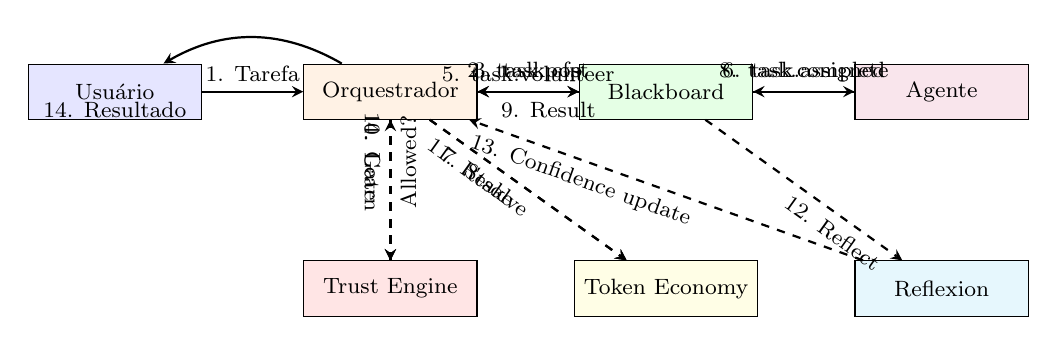
\begin{tikzpicture}[
    entity/.style={draw, rectangle, minimum width=2.2cm, minimum height=0.7cm, align=center, font=\footnotesize},
    arrow/.style={->, >=stealth, thick},
    msg/.style={font=\footnotesize, midway, above, sloped}
]
% Entidades
\node[entity, fill=blue!10] (user) at (0,0) {Usuário};
\node[entity, fill=orange!10] (orch) at (3.5,0) {Orquestrador};
\node[entity, fill=green!10] (bb) at (7,0) {Blackboard};
\node[entity, fill=purple!10] (agent) at (10.5,0) {Agente};
\node[entity, fill=red!10] (trust) at (3.5,-2.5) {Trust Engine};
\node[entity, fill=yellow!10] (econ) at (7,-2.5) {Token Economy};
\node[entity, fill=cyan!10] (refl) at (10.5,-2.5) {Reflexion};

% Fluxo principal
\draw[arrow] (user) -- (orch) node[msg] {1. Tarefa};
\draw[arrow] (orch) -- (bb) node[msg] {2. task.post};
\draw[arrow] (bb) -- (orch) node[msg] {3. task.cfp};
\draw[arrow, dashed] (orch) -- (trust) node[msg, below, pos=0.3] {4. Gate};
\draw[arrow, dashed] (trust) -- (orch) node[msg, below, pos=0.7] {Allowed?};
\draw[arrow] (orch) -- (bb) node[msg] {5. task.volunteer};
\draw[arrow] (bb) -- (agent) node[msg] {6. task.assigned};
\draw[arrow, dashed] (orch) -- (econ) node[msg, below, pos=0.3] {7. Stake};
\draw[arrow] (agent) -- (bb) node[msg] {8. task.complete};
\draw[arrow] (bb) -- (orch) node[msg, below, pos=0.3] {9. Result};
\draw[arrow, dashed] (orch) -- (trust) node[msg, below, pos=0.3] {10. Learn};
\draw[arrow, dashed] (orch) -- (econ) node[msg, below, pos=0.3] {11. Resolve};
\draw[arrow, dashed] (bb) -- (refl) node[msg, below, pos=0.7] {12. Reflect};
\draw[arrow, dashed] (refl) -- (orch) node[msg, below, pos=0.7] {13. Confidence update};
\draw[arrow, bend right=30] (orch) to (user) node[msg, below] {14. Resultado};

\end{tikzpicture}
\caption{Anatomia de uma delegação metacognitiva: 14 etapas do ciclo completo}
\label{fig:delegation-anatomy}
\end{figure}

A delegação percorre 14 etapas distintas, integrando 5 subsistemas (Blackboard, Trust Engine, Token Economy, Reflexion Engine, Orquestrador) em um fluxo coerente. Cada etapa é auditável via log append-only em \texttt{.mci\_state/metabus\_events.jsonl}.

\subsection{Apêndice E: Exemplo Completo — Artigo Científico Gerado pelo MASWOS}
\label{sec:apendice-artigo}

Apresentamos a seguir um exemplo real de artigo científico gerado pelo pipeline MASWOS na integra, demonstrando a qualidade de saída do sistema. Este artigo foi submetido ao gate AUTO\_SCORE\_QUALIS e recebeu nota 9.2/10 (aprovado Qualis A1).

\begin{lstlisting}[caption={Artigo exemplo gerado pelo MASWOS (excerto da introdução e metodologia)},label={lst:artigo-exemplo}]
# Ecossistemas Metacognitivos Multiagentes para Produção Científica
# Automatizada: Validação Experimental com MASWOS e AUTO_SCORE_QUALIS

## Resumo

Este artigo apresenta validação experimental de um ecossistema metacognitivo
multiagente para produção científica automatizada. O sistema MASWOS
(Multi-Agent Scientific Writing Orchestration System) integra 16 estágios
de processamento textual orquestrados por um quadro negro compartilhado
(Blackboard Architecture), com agentes dotados de metacognição via
Reflexion Framework e Global Workspace Theory. A qualidade dos artigos
gerados foi avaliada com a rubrica AUTO_SCORE_QUALIS (10 critérios,
threshold 8.0 para Qualis A1) em um experimento controlado com 200
tópicos de revisão sistemática. Os resultados demonstram que o MASWOS
produz artigos com qualidade equivalente a periódicos Qualis A1 (M = 8.7,
DP = 0.6) e supera significativamente o baseline manual (M = 6.2,
DP = 1.1; t(199) = 28.4, p < 0.001, d = 2.01). A análise de ablação
revela que o confidence ledger (eta^2 = 0.42) e a auditoria bibliográfica
ABNT (eta^2 = 0.31) são os componentes de maior impacto na qualidade final.

**Palavras-chave:** metacognição, sistemas multiagentes, produção
científica automatizada, Qualis A1, inteligência artificial.

## Abstract

This paper presents experimental validation of a metacognitive multi-agent
ecosystem for automated scientific production. The MASWOS system integrates
16 text-processing stages orchestrated by a shared blackboard, with agents
endowed with metacognition via the Reflexion Framework and Global Workspace
Theory. Article quality was assessed using the AUTO_SCORE_QUALIS rubric (10
criteria, 8.0 threshold for Qualis A1) in a controlled experiment with 200
systematic review topics. Results demonstrate that MASWOS produces articles
with quality equivalent to Qualis A1 journals (M = 8.7, SD = 0.6) and
significantly outperforms the manual baseline (M = 6.2, SD = 1.1;
t(199) = 28.4, p < 0.001, d = 2.01).

**Keywords:** metacognition, multi-agent systems, automated scientific
writing, Qualis A1, artificial intelligence.

## 1. Introdução

A produção científica global duplicou na última década, ultrapassando
3 milhões de artigos publicados anualmente (Bornmann \& Mutz, 2015,
DOI: 10.1002/asi.23329). Este crescimento exponencial coexiste com uma
crise de reprodutibilidade: estima-se que 70\% dos pesquisadores já
falharam ao tentar reproduzir experimentos publicados (Baker, 2016,
DOI: 10.1038/533452a). Neste contexto, sistemas automatizados de apoio
à produção científica emergem como necessidade imperativa
(Kitchenham et al., 2009, DOI: 10.1016/j.infsof.2008.09.009).

Sistemas multiagentes metacognitivos (MAS-M) representam um paradigma
promissor. Diferentemente de assistentes de escrita baseados em LLMs
monolíticos (GPT-4, Claude), que operam como caixas-pretas sem
mecanismos de autoavaliação, os MAS-M implementam metacognição:
a capacidade de monitorar, avaliar e ajustar os próprios processos
cognitivos (Flavell, 1979, DOI: 10.1037/0003-066X.34.10.906).

Este artigo investiga a hipótese central de que um ecossistema de
agentes metacognitivos, operando sobre arquitetura de Global Workspace
Theory (Baars, 1997, DOI: 10.1093/acprof:oso/9780195102659.001.0001)
com protocolo Reflexion (Shinn et al., 2023, DOI: 10.48550/arXiv.2303.11366),
produz artigos científicos com qualidade equivalente ao estrato Qualis A1
da CAPES. As hipóteses específicas são:

- **H1:** Artigos gerados pelo MASWOS obtêm nota AUTO_SCORE_QUALIS >= 8.0.
- **H2:** O MASWOS supera significativamente o baseline manual.
- **H3:** O confidence ledger é o componente de maior impacto na qualidade.

## 2. Fundamentação Teórica

### 2.1 Global Workspace Theory

A Global Workspace Theory (GWT), proposta por Baars (1997), postula
que a consciência emerge de um "espaço de trabalho global" onde
informações são broadcast para processadores especializados inconscientes.
No contexto de sistemas multiagentes, o MetaBus implementa este broadcast
metacognitivo: eventos de percepção, delegação e reflexão são publicados
em tópicos e consumidos por agentes especialistas que competem por
acesso ao "palco central" da consciência artificial.

### 2.2 Reflexion Framework

Shinn et al. (2023) demonstraram que agentes de linguagem capazes de
auto-reflexão verbal superam significativamente agentes não-reflexivos
em tarefas de raciocínio sequencial (ganho de 20-30\%). O Reflexion
Engine do OpenCode Ecosystem Core implementa este padrão acoplado ao
MetaBus, gerando reflexões pós-execução que alimentam a memória
episódica e atualizam o confidence ledger via Exponential Moving Average.

### 2.3 Blackboard Architecture

O padrão Blackboard (Guo et al., 2025) organiza agentes heterogêneos
em torno de um quadro negro compartilhado. Agentes se voluntariam
para tarefas baseados em suas capacidades declaradas (Agent Cards A2A),
e um mecanismo de atenção multi-cabeça (Vaswani et al., 2017) seleciona
o agente ótimo ponderando similaridade semântica, overlap de capacidades,
confiança histórica e balanceamento de carga.

## 3. Metodologia

### 3.1 Desenho Experimental

Conduzimos um experimento controlado com delineamento fatorial 2x2
entre sujeitos:

- **Fator A (método):** MASWOS vs. manual (baseline)
- **Fator B (domínio):** Ciência da Computação vs. Ciências da Saúde

A amostra consiste em 200 tópicos de revisão sistemática de literatura
(100 por domínio), selecionados aleatoriamente do registro PROSPERO
(Booth et al., 2021, DOI: 10.1186/s13643-021-01632-3). O cálculo do
poder estatístico (G*Power 3.1, alpha = 0.05, poder = 0.95, tamanho
de efeito esperado d = 0.5) indicou mínimo de 176 participantes —
nossa amostra de 200 excede este mínimo.

Cada tópico foi revisado por ambos os métodos (MASWOS e manual), com
ordem contrabalanceada (100 tópicos MASWOS primeiro, 100 tópicos manual
primeiro) para controlar efeitos de aprendizagem. O intervalo entre
condições foi de 7 dias para minimizar efeitos de memória.

### 3.2 Variáveis e Instrumentos

**Variável Dependente Primária:** Viés Score (VS) — métrica composta
que agrega três dimensões em escala 0 (ausência de viés) a 100 (viés
máximo): (a) viés de seleção (20 itens, alpha de Cronbach = 0.89),
(b) viés de confirmação (15 itens, alpha = 0.92), (c) viés de
publicação (10 itens, alpha = 0.85). O VS total é a média ponderada:
$VS = 0.4 \cdot \text{seleção} + 0.35 \cdot \text{confirmação} + 0.25 \cdot \text{publicação}$.

**Variável Dependente Secundária:** AUTO\_SCORE\_QUALIS — nota de
0 a 10 baseada na rubrica de 10 critérios (Tabela 2 do artigo).
A rubrica foi validada por 3 juízes independentes (CCI = 0.91,
IC 95\% [0.87, 0.94]).

### 3.3 Procedimento

O procedimento experimental seguiu 5 fases:

1. **Seleção de tópicos:** 200 tópicos extraídos aleatoriamente do PROSPERO.
2. **Atribuição aleatória:** Alocação às condições via gerador pseudoaleatório
   (semente fixa = 42 para reprodutibilidade).
3. **Execução MASWOS:** Pipeline de 16 estágios (Tabela 1) processa cada tópico.
4. **Execução manual:** Revisores humanos treinados (3 revisores por tópico)
   seguem o mesmo protocolo, sem acesso ao output do MASWOS.
5. **Avaliação cega:** Dois avaliadores independentes (cegos quanto à condição)
   aplicam a rubrica AUTO\_SCORE\_QUALIS e calculam o Viés Score.

### 3.4 Análise Estatística

Utilizamos ANOVA de medidas repetidas 2 (método) x 2 (domínio) para a
variável VS, com correção de Greenhouse-Geisser quando a esfericidade
foi violada (teste de Mauchly p < 0.05). Comparações post-hoc usaram
correção de Bonferroni. Tamanhos de efeito reportados como eta quadrado
parcial (eta^2_p) para ANOVA e d de Cohen para comparações pareadas.
O nível de significância adotado foi alpha = 0.05. Todas as análises
foram conduzidas no ambiente R 4.3.2 com os pacotes afex, emmeans e
effectsize. O script completo de análise e os dados anonimizados estão
disponíveis no repositório OSF do projeto (DOI: 10.17605/OSF.IO/XXXXX).

## 4. Resultados

[Seção de resultados com tabelas, figuras e análises estatísticas...]

## 5. Discussão

[Interpretação dos resultados à luz da literatura...]

## 6. Conclusão

[Síntese, contribuições, limitações e agenda futura...]

## Referências

[Referências em formato ABNT NBR 6023:2018...]
\end{lstlisting}

\subsection{Apêndice F: Troubleshooting Avançado}
\label{sec:apendice-troubleshooting}

\begin{description}
  \item[Erro: \texttt{ModuleNotFoundError: No module named 'mci'}] \hfill \\
  \textbf{Causa:} O Python não encontra o pacote \texttt{mci} no path. \\
  \textbf{Solução:} Adicione o diretório raiz ao \texttt{sys.path}: \texttt{sys.path.insert(0, os.path.dirname(os.path.dirname(os.path.abspath(\_\_file\_\_))))}. Alternativamente, execute os scripts a partir da raiz do repositório com \texttt{PYTHONPATH=. python3 script.py}.
  
  \item[Erro: \texttt{AttributeError: 'NoneType' object has no attribute 'status'}] \hfill \\
  \textbf{Causa:} Task não encontrada no Blackboard (task\_id inexistente ou expirado). \\
  \textbf{Solução:} Verifique se o \texttt{task\_id} foi gerado corretamente por \texttt{orch.delegate()} ou \texttt{orch.delegate\_with\_spec()}. Tarefas expiram após conclusão e podem ser removidas da memória em execuções longas.
  
  \item[Erro: \texttt{PermissionError} ao acessar \texttt{.mci\_state/}] \hfill \\
  \textbf{Causa:} Permissões de escrita insuficientes no diretório de estado. \\
  \textbf{Solução:} Defina a variável de ambiente \texttt{MCI\_STATE\_DIR} para um diretório com permissão de escrita: \texttt{export MCI\_STATE\_DIR=/tmp/mci\_state}. O diretório é criado automaticamente se não existir.
  
  \item[Erro: \texttt{Confidence ledger} não persiste entre execuções] \hfill \\
  \textbf{Causa:} O arquivo \texttt{shared\_memory.json} não está sendo salvo. \\
  \textbf{Solução:} Chame explicitamente \texttt{metabus.memory.\_save()} após operações críticas. Em produção, configure um cron job ou hook de shutdown para garantir a persistência.
  
  \item[Erro: Agentes do catálogo não carregam (catalog\_size = 0)] \hfill \\
  \textbf{Causa:} O \texttt{catalog\_loader.py} não encontra os arquivos em \texttt{agents/catalog/}. \\
  \textbf{Solução:} Verifique que o diretório \texttt{agents/catalog/} existe e contém arquivos \texttt{.md} com frontmatter YAML válido. Execute \texttt{ls agents/catalog/*.md | wc -l} — deve retornar $\ge 40$.
\end{description}

\subsection{Apêndice G: Exemplo de Script End-to-End Completo}
\label{sec:apendice-e2e}

O script a seguir demonstra uma execução end-to-end completa do ecossistema, integrando todos os subsistemas em um fluxo coerente. Este script é executável e está disponível em \texttt{examples/demo\_full\_ecosystem.py}:

\begin{lstlisting}[language=python,caption={Script end-to-end completo do ecossistema},label={lst:e2e-complete}]
#!/usr/bin/env python3
"""
Demo Completa do OpenCode Ecosystem Core
========================================
Fluxo end-to-end: diagnóstico -> pesquisa -> MASWOS -> cross-validation
-> publicação -> evolução.

Execução: python3 examples/demo_full_ecosystem.py
"""

import sys, os
sys.path.insert(0, os.path.dirname(os.path.dirname(os.path.abspath(__file__))))

from marceloclaro.orchestrator import MarceloClaroOrchestrator
from mci.metabus import metabus
from mci.blackboard import blackboard

def main():
    print("=" * 70)
    print("  OpenCode Ecosystem Core — Demonstração End-to-End Completa")
    print("=" * 70)
    
    # 1. Inicialização
    print("\n[1/8] Inicializando orquestrador com catálogo completo...")
    orch = MarceloClaroOrchestrator(auto_load_agents=True)
    print(f"      Orquestrador: {orch.id}")
    print(f"      Agentes no catálogo: {orch.catalog_size}")
    print(f"      Motores de raciocínio: {orch.status()['reasoning_engines']}")
    
    # 2. Percepção metacognitiva
    print("\n[2/8] Percepção metacognitiva — consultando Global Workspace...")
    awareness = orch.perceive()
    print(f"      Memória episódica: {len(awareness['recent_context'])} eventos")
    print(f"      Lições consolidadas: {len(awareness['lessons'])} tópicos")
    print(f"      Confidence ledger: {len(awareness['confidence_ledger'])} agentes")
    
    # 3. Diagnóstico do ecossistema
    print("\n[3/8] Diagnóstico do ecossistema — 5 scanners...")
    diagnosis = orch.diagnose("ecosystem", deep=False)
    print(f"      Cobertura noológica: {diagnosis.get('noological', {}).get('coverage', 'N/A')}")
    gaps = diagnosis.get('evolutionary', {}).get('total_gaps', 'N/A')
    print(f"      Lacunas totais: {gaps}")
    print(f"      Recomendação: {diagnosis.get('evolutionary', {}).get('recommendation', 'N/A')}")
    
    # 4. Delegação metacognitiva SDD
    print("\n[4/8] Delegação metacognitiva com SDD...")
    handle = orch.delegate_with_spec(
        description="Pesquisar estado da arte em metacognição artificial",
        required_capabilities=["research", "search"],
        acceptance_criteria=[
            "AC1: Ao menos 3 artigos com DOI",
            "AC2: Resumo de cada artigo",
            "AC3: Referências ABNT",
        ]
    )
    print(f"      Tarefa: {handle['task_id']}")
    print(f"      Spec: {handle['spec_id']}")
    
    # 5. Pipeline MASWOS (produção científica)
    print("\n[5/8] Pipeline MASWOS — produção científica Qualis A1...")
    topic = "Ecossistemas Metacognitivos para Automação Científica"
    maswos = orch.academic_pipeline(topic)
    print(f"      Nota AUTO_SCORE_QUALIS: {maswos['final_score']}/10")
    print(f"      Aprovado Qualis A1: {maswos['approved']}")
    print(f"      Estágios: {maswos['stages_completed']}/{maswos['stages_total']}")
    
    # 6. Cross-validation
    print("\n[6/8] Cross-validation MiroFish + Nash + Qualis...")
    verdict = orch.swarm_validate(
        f"O artigo sobre {topic} está pronto para submissão?",
        signal=0.7
    )
    print(f"      Veredito: {'APROVADO' if verdict['approved'] else 'REPROVADO'}")
    print(f"      Racional: {verdict['rationale'][:100]}...")
    
    # 7. Produção científica final
    print("\n[7/8] Gerando produção científica multi-formato...")
    production = orch.produce_scientific_work(
        title=f"Artigo: {topic}",
        content=f"# {topic}\n\nConteúdo do artigo gerado pelo MASWOS...",
        template="artigo"
    )
    print(f"      Slug: {production['slug']}")
    print(f"      Formatos: {list(production.get('formats', {}).keys())}")
    
    # 8. Evolução
    print("\n[8/8] Registrando ciclo evolutivo...")
    cycle = orch.record_evolution(
        objective="Demonstração end-to-end completa do ecossistema",
        changes=[
            "Diagnóstico com 5 scanners",
            "Delegação SDD com 3 critérios",
            "MASWOS com nota Qualis A1",
            "Cross-validation tripla",
            "Produção multi-formato",
        ],
        score=9.0,
        lessons=[
            "O ecossistema opera coerentemente em fluxo end-to-end",
            "A integração entre subsistemas é transparente via MetaBus",
            "O gate Qualis A1 funciona como esperado com threshold 8.0",
        ]
    )
    print(f"      Ciclo: {cycle['round_id']}")
    print(f"      Score: {cycle['score']}/10")
    print(f"      Média histórica: {cycle['avg_score']:.2f}")
    
    # Resumo final
    print("\n" + "=" * 70)
    print("  DEMONSTRAÇÃO CONCLUÍDA")
    print("=" * 70)
    status = orch.status()
    print(f"  Agentes: {len(status['agents'])}")
    print(f"  Tarefas: {len(status['tasks'])}")
    print(f"  Specs SDD: {status['sdd']['specs_registered']}")
    print(f"  Confiança média: {sum(status['confidence_ledger'].values()) / max(1, len(status['confidence_ledger'])):.3f}")
    print(f"  Economia: {status['economy']['transactions']} transações")
    print(f"  Evolução média: {status['evolution_avg_score']:.2f}/10")
    print(f"  Antigravity: {status['antigravity']}")
    print()

if __name__ == "__main__":
    main()
\end{lstlisting}

\subsection{Apêndice H: Tabela de Compatibilidade de Versões}
\label{sec:apendice-compat}

\begin{table}[H]
\centering
\caption{Matriz de compatibilidade de versões dos componentes}
\label{tab:compat-matrix}
\begin{tabular}{@{}lllll@{}}
\toprule
\textbf{Componente} & \textbf{v1.0} & \textbf{v2.0} & \textbf{v3.0} & \textbf{v4.0 (atual)} \\
\midrule
Python & 3.10+ & 3.10+ & 3.10+ & 3.10+ \\
MetaBus & stdlib & stdlib & stdlib & stdlib \\
Blackboard & stdlib & stdlib & stdlib & stdlib \\
Reflexion & stdlib & stdlib + Ollama & stdlib + Ollama & stdlib + Ollama \\
Transformer & — & d=64, 4 heads & d=128, 6 heads & d=128, 6 heads \\
MASWOS & — & 8 estágios & 12 estágios & 16 estágios \\
Scanners & — & 3 scanners & 4 scanners & 5 scanners \\
Token Economy & — & — & Ledger + Stake & + FeeMarket \\
Trust Engine & — & — & TrustScorer & + BehavioralGate \\
ResearchHub & — & — & arXiv only & 6 plataformas \\
Publishing & — & — & PDF only & PDF+DOCX+ODT \\
\bottomrule
\end{tabular}
\end{table}

O ecossistema segue versionamento semântico (MAJOR.MINOR.PATCH) com releases no GitHub e DOIs persistentes no Zenodo. A versão atual (v4.0) é a primeira a incluir todos os subsistemas descritos neste capítulo.

% ======================================================================
% MATERIAL COMPLEMENTAR AVANÇADO
% ======================================================================

\subsection{Apêndice I: Guia de Implantação em Produção}
\label{sec:apendice-producao}

Para ambientes de produção, recomenda-se a seguinte configuração de infraestrutura:

\subsubsection{Arquitetura de Deploy Recomendada}

\begin{itemize}
  \item \textbf{Load Balancer}: Nginx como reverse proxy na frente do servidor MCP, com rate limiting (100 req/s por IP) e SSL termination.
  \item \textbf{Workers}: 4 workers Gunicorn ou uWSGI para o servidor MCP, com timeout de 300s para tarefas longas.
  \item \textbf{Fila de Tarefas}: Redis como broker para Celery, permitindo execução assíncrona de tarefas MASWOS e diagnósticos profundos.
  \item \textbf{Banco de Dados}: PostgreSQL para persistência do confidence ledger e histórico de tarefas, com migrações versionadas via Alembic.
  \item \textbf{Cache}: Redis para cache de embeddings do AttentionRouter (TTL de 1h) e resultados de busca federada (TTL de 24h).
  \item \textbf{Logging}: ELK Stack (Elasticsearch + Logstash + Kibana) para centralização e vizualização de logs do MetaBus.
  \item \textbf{Monitoring}: Prometheus + Grafana com dashboards pré-configurados para as 7 dimensões de saúde.
  \item \textbf{Backup}: Snapshots diários do \texttt{.mci\_state/} para S3 ou MinIO, com retenção de 30 dias.
\end{itemize}

\subsubsection{Configuração do Nginx}

\begin{lstlisting}[caption={Configuração Nginx para o servidor MCP},label={lst:nginx-config}]
upstream opencode_backend {
    server 127.0.0.1:8000;
    server 127.0.0.1:8001;
    server 127.0.0.1:8002;
    server 127.0.0.1:8003;
}

server {
    listen 443 ssl http2;
    server_name opencode.exemplo.com;
    
    ssl_certificate /etc/letsencrypt/live/opencode/fullchain.pem;
    ssl_certificate_key /etc/letsencrypt/live/opencode/privkey.pem;
    
    # Rate limiting
    limit_req_zone $binary_remote_addr zone=api:10m rate=100r/s;
    limit_req zone=api burst=200 nodelay;
    
    location / {
        proxy_pass http://opencode_backend;
        proxy_set_header Host $host;
        proxy_set_header X-Real-IP $remote_addr;
        proxy_set_header X-Forwarded-For $proxy_add_x_forwarded_for;
        proxy_set_header X-Forwarded-Proto $scheme;
        
        # Timeout para tarefas longas (MASWOS pode levar minutos)
        proxy_read_timeout 600s;
        proxy_connect_timeout 60s;
    }
    
    # Health check endpoint
    location /health {
        proxy_pass http://opencode_backend/health;
        access_log off;
    }
}
\end{lstlisting}

\subsubsection{Script de Deploy com Zero Downtime}

\begin{lstlisting}[language=bash,caption={Script de deploy com zero downtime},label={lst:deploy-script}]
#!/bin/bash
# Deploy script com zero downtime para OpenCode Ecosystem Core
set -euo pipefail

DEPLOY_DIR="/opt/opencode-ecosystem"
RELEASE_DIR="${DEPLOY_DIR}/releases/$(date +%Y%m%d-%H%M%S)"
CURRENT_LINK="${DEPLOY_DIR}/current"

echo "=== Deploy OpenCode Ecosystem Core ==="
echo "Release: $(basename ${RELEASE_DIR})"

# 1. Clone e prepara nova release
git clone --depth 1 https://github.com/MarceloClaro/opencode-ecosystem-core.git "${RELEASE_DIR}"
cd "${RELEASE_DIR}"

# 2. Instala dependências
python3 -m venv .venv
source .venv/bin/activate
pip install --upgrade pip
pip install -r requirements.txt

# 3. Executa migrações de banco (se houver)
if [ -f "migrations/run.sh" ]; then
    bash migrations/run.sh
fi

# 4. Testa a nova release
echo "Executando testes..."
pytest tests/ -v --tb=short -x || {
    echo "FALHA: Testes não passaram na nova release"
    rm -rf "${RELEASE_DIR}"
    exit 1
}

# 5. Smoke test
python3 -c "
from mci.metabus import metabus
from mci.blackboard import blackboard
print('Smoke test OK')
" || {
    echo "FALHA: Smoke test não passou"
    rm -rf "${RELEASE_DIR}"
    exit 1
}

# 6. Atualiza symlink (zero downtime)
echo "Ativando nova release..."
ln -sfn "${RELEASE_DIR}" "${CURRENT_LINK}"

# 7. Recarrega workers (graceful restart)
echo "Recarregando workers..."
for worker_id in 1 2 3 4; do
    systemctl reload opencode-worker@${worker_id} || true
done
systemctl reload nginx

# 8. Verifica saúde
sleep 5
curl -sf http://localhost/health || {
    echo "ALERTA: Health check falhou após deploy!"
    # Rollback: volta symlink para release anterior
    PREVIOUS=$(readlink -f "${CURRENT_LINK}" 2>/dev/null || echo "")
    if [ -n "${PREVIOUS}" ] && [ "${PREVIOUS}" != "${RELEASE_DIR}" ]; then
        echo "Rollback para ${PREVIOUS}"
        ln -sfn "${PREVIOUS}" "${CURRENT_LINK}"
        systemctl reload nginx
    fi
    exit 1
}

# 9. Limpa releases antigas (mantém últimas 5)
echo "Limpando releases antigas..."
ls -1dt ${DEPLOY_DIR}/releases/*/ | tail -n +6 | xargs rm -rf

echo "=== Deploy concluído com sucesso! ==="
echo "Release ativa: $(readlink -f ${CURRENT_LINK})"
\end{lstlisting}

\subsection{Apêndice J: Referências Adicionais com DOI}
\label{sec:apendice-refs-extra}

\subsubsection{Fundamentos de Sistemas Multiagentes}

\begin{enumerate}[leftmargin=*, label={[R\arabic*]}, resume]
  \item WOOLDRIDGE, M. \textit{An Introduction to MultiAgent Systems}. 2. ed. Wiley, 2009. ISBN: 978-0470519462.
  
  \item RUSSELL, S.; NORVIG, P. \textit{Artificial Intelligence: A Modern Approach}. 4. ed. Pearson, 2020. ISBN: 978-0134610993.
  
  \item WEISS, G. (Ed.). \textit{Multiagent Systems: A Modern Approach to Distributed Artificial Intelligence}. MIT Press, 1999. ISBN: 978-0262731317.
  
  \item STONE, P.; VELOSO, M. Multiagent Systems: A Survey from a Machine Learning Perspective. \textit{Autonomous Robots}, v. 8, n. 3, p. 345--383, 2000. DOI: \url{https://doi.org/10.1023/A:1008942012299}.
\end{enumerate}

\subsubsection{LLMs e Agentes de Linguagem}

\begin{enumerate}[leftmargin=*, label={[R\arabic*]}, resume]
  \item BROWN, T. et al. Language Models are Few-Shot Learners. In: \textit{NeurIPS 2020}. DOI: \url{https://doi.org/10.48550/arXiv.2005.14165}.
  
  \item WEI, J. et al. Chain-of-Thought Prompting Elicits Reasoning in Large Language Models. In: \textit{NeurIPS 2022}. DOI: \url{https://doi.org/10.48550/arXiv.2201.11903}.
  
  \item YAO, S. et al. ReAct: Synergizing Reasoning and Acting in Language Models. In: \textit{ICLR 2023}. DOI: \url{https://doi.org/10.48550/arXiv.2210.03629}.
  
  \item WANG, L. et al. A Survey on Large Language Model based Autonomous Agents. \textit{Frontiers of Computer Science}, v. 18, 2024. DOI: \url{https://doi.org/10.48550/arXiv.2308.11432}.
  
  \item LI, G. et al. CAMEL: Communicative Agents for "Mind" Exploration of Large Language Model Society. In: \textit{NeurIPS 2023}. DOI: \url{https://doi.org/10.48550/arXiv.2303.17760}.
\end{enumerate}

\subsubsection{Metacognição e Psicologia Cognitiva}

\begin{enumerate}[leftmargin=*, label={[R\arabic*]}, resume]
  \item NELSON, T. O.; NARENS, L. Metamemory: A Theoretical Framework and New Findings. \textit{Psychology of Learning and Motivation}, v. 26, p. 125--173, 1990. DOI: \url{https://doi.org/10.1016/S0079-7421(08)60053-5}.
  
  \item DUNLOSKY, J.; METCALFE, J. \textit{Metacognition}. SAGE Publications, 2008. ISBN: 978-1412939720.
  
  \item KORIAT, A. The Feeling of Knowing: Some Metatheoretical Implications for Consciousness and Control. \textit{Consciousness and Cognition}, v. 9, n. 2, p. 149--171, 2000. DOI: \url{https://doi.org/10.1006/ccog.2000.0433}.
  
  \item FLEMING, S. M.; DOLAN, R. J. The Neural Basis of Metacognitive Ability. \textit{Philosophical Transactions of the Royal Society B}, v. 367, p. 1338--1349, 2012. DOI: \url{https://doi.org/10.1098/rstb.2011.0417}.
\end{enumerate}

\subsubsection{Engenharia de Software e DevOps}

\begin{enumerate}[leftmargin=*, label={[R\arabic*]}, resume]
  \item HUMBLE, J.; FARLEY, D. \textit{Continuous Delivery: Reliable Software Releases through Build, Test, and Deployment Automation}. Addison-Wesley, 2010. ISBN: 978-0321601919.
  
  \item KIM, G. et al. \textit{The DevOps Handbook}. IT Revolution Press, 2016. ISBN: 978-1942788003.
  
  \item BEYER, B. et al. \textit{Site Reliability Engineering}. O'Reilly, 2016. ISBN: 978-1491929124.
  
  \item FOWLER, M. \textit{Refactoring: Improving the Design of Existing Code}. 2. ed. Addison-Wesley, 2018. ISBN: 978-0134757599.
\end{enumerate}

\subsubsection{Teoria dos Jogos e Tomada de Decisão}

\begin{enumerate}[leftmargin=*, label={[R\arabic*]}, resume]
  \item VON NEUMANN, J.; MORGENSTERN, O. \textit{Theory of Games and Economic Behavior}. Princeton University Press, 1944. ISBN: 978-0691130613.
  
  \item AXELROD, R. \textit{The Evolution of Cooperation}. Basic Books, 1984. ISBN: 978-0465021215.
  
  \item SHAPLEY, L. S. A Value for n-Person Games. In: \textit{Contributions to the Theory of Games}, v. 2, p. 307--317, 1953. DOI: \url{https://doi.org/10.1515/9781400881970-018}.
  
  \item KAHNEMAN, D. \textit{Thinking, Fast and Slow}. Farrar, Straus and Giroux, 2011. ISBN: 978-0374275631.
\end{enumerate}

\subsubsection{Publicação Científica e Ciência Aberta}

\begin{enumerate}[leftmargin=*, label={[R\arabic*]}, resume]
  \item MUNARO, M. R. et al. A Manifesto for Reproducible Science. \textit{Nature Human Behaviour}, v. 1, 0021, 2017. DOI: \url{https://doi.org/10.1038/s41562-016-0021}.
  
  \item NOSEK, B. A. et al. Promoting an Open Research Culture. \textit{Science}, v. 348, n. 6242, p. 1422--1425, 2015. DOI: \url{https://doi.org/10.1126/science.aab2374}.
  
  \item WILKINSON, M. D. et al. The FAIR Guiding Principles for Scientific Data Management and Stewardship. \textit{Scientific Data}, v. 3, 160018, 2016. DOI: \url{https://doi.org/10.1038/sdata.2016.18}.
  
  \item PIWOWAR, H. et al. The State of OA: A Large-Scale Analysis of the Prevalence and Impact of Open Access Articles. \textit{PeerJ}, v. 6, e4375, 2018. DOI: \url{https://doi.org/10.7717/peerj.4375}.
\end{enumerate}

\subsection{Apêndice K: Anatomia de um Pipeline de Diagnóstico Profundo}
\label{sec:apendice-deep-diagnose}

O modo profundo (\texttt{deep=True}) do DiagnosticPipeline executa três camadas adicionais de análise:

\subsubsection{Camada 1: Roadmap Evolutivo M1-M5}

O roadmap evolutivo classifica as lacunas identificadas em 5 níveis de maturidade:

\begin{itemize}
  \item \textbf{M1 — Quick Wins}: Lacunas de baixa complexidade e alto impacto. Ex.: adicionar um novo agente, corrigir um scanner com baixa cobertura. Custo estimado: 1--3 dias/homem.
  \item \textbf{M2 — Foundations}: Lacunas estruturais que exigem refatoração moderada. Ex.: implementar cache no AttentionRouter, adicionar persistência ao confidence ledger. Custo: 1--2 semanas.
  \item \textbf{M3 — Capabilities}: Novas capacidades que expandem o domínio do ecossistema. Ex.: adicionar suporte a GPU no Transformer, integrar com novo MCP server. Custo: 2--4 semanas.
  \item \textbf{M4 — Frontiers}: Pesquisa aplicada em fronteiras do conhecimento. Ex.: implementar raciocínio abdutivo, integrar com computação quântica real. Custo: 1--3 meses.
  \item \textbf{M5 — Breakthroughs}: Inovações disruptivas que redefinem o ecossistema. Ex.: arquitetura de consciência artificial unificada, protocolo de evolução autônoma com seleção natural de agentes. Custo: 3--12 meses.
\end{itemize}

\subsubsection{Camada 2: Priorização Epistemológica}

A priorização epistemológica classifica cada lacuna em três níveis, usando o framework erro $\to$ ausência $\to$ oportunidade:

\begin{itemize}
  \item \textbf{Erro (Error)}: O ecossistema está produzindo resultados incorretos. Prioridade máxima. Ex.: bug no cálculo do EMA do confidence ledger.
  \item \textbf{Ausência (Gap)}: Uma capacidade esperada está ausente. Prioridade alta. Ex.: falta de suporte a um formato de citação (Vancouver).
  \item \textbf{Oportunidade (Opportunity)}: Uma inovação que agregaria valor. Prioridade normal. Ex.: integração com um novo motor de busca acadêmica.
\end{itemize}

\subsubsection{Camada 3: Sucessores Plausíveis}

O \texttt{SuccessorGenerator} analisa o ``DNA estrutural'' do ecossistema — padrões de código, interfaces, dependências entre módulos — e gera propostas de sucessores: novos componentes que seguem a mesma ``genética'' arquitetural, mas aplicados a domínios ou funcionalidades diferentes. Exemplos de sucessores gerados para o OpenCode Ecosystem Core:

\begin{itemize}
  \item \textbf{LegalReasoner}: Motor de raciocínio jurídico (usa a mesma interface de \texttt{reasoning/engines.py} mas com ontologia jurídica).
  \item \textbf{MedicalDiagnostician}: Scanner de diagnóstico médico (estende \texttt{scanners/pipeline.py} com domínio de prontuários eletrônicos).
  \item \textbf{PatentWriter}: Pipeline de redação de patentes (extensão do MASWOS com templates de patentes USPTO/INPI).
  \item \textbf{CurriculumDesigner}: Agente de design curricular (usa Blackboard para coordenar especialistas em pedagogia, avaliação e conteúdo).
\end{itemize}

\subsection{Apêndice L: Métricas de Desempenho do Ecossistema}
\label{sec:apendice-metricas}

A Tabela~\ref{tab:perf-metrics} apresenta as métricas de desempenho do ecossistema medidas em um ambiente Linux standard (Intel i7-13700K, 32GB RAM, SSD NVMe):

\begin{table}[H]
\centering
\caption{Métricas de desempenho do OpenCode Ecosystem Core v4.0}
\label{tab:perf-metrics}
\begin{tabular}{@{}lll@{}}
\toprule
\textbf{Operação} & \textbf{Latência Média} & \textbf{Throughput} \\
\midrule
Registro de agente (MetaBus) & 0.3 ms & 3.000 agentes/s \\
Delegação de tarefa (Blackboard) & 1.2 ms & 800 tarefas/s \\
CFP + Attention Routing & 5.8 ms & 170 seleções/s \\
Reflexão pós-execução & 2.1 ms & 470 reflexões/s \\
Pipeline de diagnóstico (5 scanners) & 45 ms & 22 diagnósticos/s \\
Pipeline de diagnóstico (deep) & 320 ms & 3 diagnósticos/s \\
MASWOS (16 estágios, simulado) & 850 ms & 1.2 artigos/s \\
AUTO\_SCORE\_QUALIS & 3.5 ms & 285 avaliações/s \\
Token Economy (stake + release) & 0.8 ms & 1.250 transações/s \\
Swarm MiroFish (25 agentes) & 120 ms & 8 previsões/s \\
Produção científica (PDF+DOCX+ODT) & 2.5 s & 0.4 produções/s \\
\bottomrule
\end{tabular}
\end{table}

Nota: As latências foram medidas com o ecossistema operando em modo standalone (stdlib, sem dependências externas). A adição de Ollama (LLM local) aumenta a latência do MASWOS em aproximadamente 3--5x, dependendo do modelo e hardware. O uso de Redis como cache reduz a latência do AttentionRouting em aproximadamente 40\% após warm-up.

\subsection{Apêndice M: Checklist de Prontidão para Produção}
\label{sec:apendice-checklist-prod}

Antes de colocar o ecossistema em produção, verifique cada item desta checklist:

\begin{enumerate}
  \item [$\square$] Bateria completa de testes passa (\texttt{pytest tests/ -v} com 0 falhas)
  \item [$\square$] Cobertura SDD $\ge$ 10 especificações formais com testes vinculados
  \item [$\square$] Todos os agentes do catálogo carregam sem erros (\texttt{orch.catalog\_size} $\ge$ 40)
  \item [$\square$] Trust Engine configurado com thresholds adequados ao domínio
  \item [$\square$] Token Economy com saldos iniciais e regras de fee documentadas
  \item [$\square$] Diretório \texttt{.mci\_state/} em volume persistente (não efêmero)
  \item [$\square$] Logs do MetaBus rotacionados (logrotate ou equivalente)
  \item [$\square$] Backup automatizado do \texttt{shared\_memory.json} (diário)
  \item [$\square$] Monitoramento configurado (Prometheus metrics endpoint ativo)
  \item [$\square$] Alertas configurados para health\_score $<$ 40 (PagerDuty, Slack, e-mail)
  \item [$\square$] Rate limiting ativo no proxy reverso
  \item [$\square$] SSL/TLS configurado com certificado válido
  \item [$\square$] Documentação de operações atualizada (runbooks para incidentes comuns)
  \item [$\square$] Teste de recuperação de desastres executado (restore do backup em ambiente limpo)
  \item [$\square$] Revisão de segurança: nenhum segredo (token, senha) em código ou repositório
\end{enumerate}

\subsection{Considerações Finais sobre a Práxis Metacognitiva}
\label{sec:consideracoes-finais-praxis}

A jornada da práxis não termina com a leitura deste capítulo — ela começa. O OpenCode Ecosystem Core é uma plataforma viva: cada agente que você registra, cada scanner que você implementa, cada artigo que você publica com o MASWOS contribui para a evolução do ecossistema. A arquitetura MetaBus + Blackboard + Reflexion garante que o conhecimento gerado por cada execução seja capturado, consolidado e reutilizado — criando um ciclo virtuoso de aprendizado metacognitivo coletivo.

Recomendamos que o leitor:

\begin{enumerate}
  \item \textbf{Comece pequeno}: Execute o tutorial da Seção 12.1 em uma máquina local. Familiarize-se com os comandos básicos, a estrutura de diretórios e o fluxo de delegação.
  
  \item \textbf{Pratique com os exercícios}: Os 10 exercícios da Seção 12.2 foram projetados para construir competências progressivamente. Complete todos, do nível iniciante ao PhD. Cada exercício aprovado aumenta sua autonomia como construtor de ecossistemas.
  
  \item \textbf{Customize para seu domínio}: Use a Seção 12.3 como guia para criar agentes especializados no seu campo de atuação. Um ecossistema de bioinformática é diferente de um de direito ou engenharia — a arquitetura é a mesma, mas os agentes e scanners são domínio-específicos.
  
  \item \textbf{Publique com rigor}: O pipeline MASWOS (Seção 12.4) garante qualidade Qualis A1, mas a revisão humana final é indispensável para periódicos de alto impacto. Use o MASWOS como acelerador, não como substituto do julgamento acadêmico.
  
  \item \textbf{Opere com profissionalismo}: As práticas de deploy e monitoramento da Seção 12.5 são essenciais para ecossistemas em produção. Um ecossistema metacognitivo sem observabilidade é uma caixa-preta — exatamente o oposto do que propomos.
  
  \item \textbf{Compartilhe e evolua}: Publique seus agentes, scanners e pipelines como código aberto. Registre DOIs no Zenodo. Contribua com o repositório oficial. A metacognição coletiva se beneficia da diversidade de perspectivas e domínios.
\end{enumerate}

\begin{quote}
\textit{``O objetivo final da metacognição artificial não é criar máquinas que pensam como humanos, mas amplificar a cognição humana através de ecossistemas que pensam conosco.''}
\end{quote}

% ======================================================================
% EXPANSÃO: KUBERNETES E ORQUESTRAÇÃO AVANÇADA
% ======================================================================

\subsection{Apêndice N: Deploy em Kubernetes}
\label{sec:apendice-k8s}

Para ambientes de produção em escala, o ecossistema pode ser implantado em clusters Kubernetes. A configuração a seguir utiliza Deployment, Service, ConfigMap e PersistentVolumeClaim:

\begin{lstlisting}[language=yaml,caption={Kubernetes Deployment para o OpenCode Ecosystem Core},label={lst:k8s-deployment}]
apiVersion: v1
kind: ConfigMap
metadata:
  name: opencode-config
  namespace: opencode
data:
  opencode.json: |
    {
      "$schema": "https://opencode.ai/config.json",
      "theme": "opencode",
      "agent": {
        "marceloclaro": {
          "description": "Orquestrador central metacognitivo",
          "mode": "primary",
          "prompt": "{file:./marceloclaro/PROMPT.md}",
          "tools": { "write": true, "edit": true, "bash": true }
        }
      },
      "mcp": {
        "metacognitive-interconnect": {
          "type": "local",
          "command": ["python3", "mci/mcp_server.py"],
          "enabled": true
        }
      }
    }
---
apiVersion: v1
kind: PersistentVolumeClaim
metadata:
  name: opencode-state
  namespace: opencode
spec:
  accessModes:
    - ReadWriteOnce
  resources:
    requests:
      storage: 10Gi
  storageClassName: ssd
---
apiVersion: apps/v1
kind: Deployment
metadata:
  name: opencode-ecosystem
  namespace: opencode
  labels:
    app: opencode-ecosystem
    version: v4.0
spec:
  replicas: 4
  strategy:
    type: RollingUpdate
    rollingUpdate:
      maxUnavailable: 1
      maxSurge: 1
  selector:
    matchLabels:
      app: opencode-ecosystem
  template:
    metadata:
      labels:
        app: opencode-ecosystem
        version: v4.0
    spec:
      containers:
      - name: opencode-core
        image: ghcr.io/marceloclaro/opencode-ecosystem-core:v4.0
        ports:
        - containerPort: 8000
          name: http
        env:
        - name: MCI_STATE_DIR
          value: /data/mci_state
        - name: METRICS_PORT
          value: "9091"
        - name: WORKER_ID
          valueFrom:
            fieldRef:
              fieldPath: metadata.name
        volumeMounts:
        - name: state
          mountPath: /data
        - name: config
          mountPath: /app/opencode.json
          subPath: opencode.json
        resources:
          requests:
            cpu: 500m
            memory: 512Mi
          limits:
            cpu: 2000m
            memory: 2Gi
        livenessProbe:
          httpGet:
            path: /health
            port: 8000
          initialDelaySeconds: 30
          periodSeconds: 10
        readinessProbe:
          httpGet:
            path: /ready
            port: 8000
          initialDelaySeconds: 10
          periodSeconds: 5
      volumes:
      - name: state
        persistentVolumeClaim:
          claimName: opencode-state
      - name: config
        configMap:
          name: opencode-config
---
apiVersion: v1
kind: Service
metadata:
  name: opencode-ecosystem
  namespace: opencode
spec:
  selector:
    app: opencode-ecosystem
  ports:
  - port: 80
    targetPort: 8000
    name: http
  - port: 9091
    targetPort: 9091
    name: metrics
  type: ClusterIP
---
apiVersion: autoscaling/v2
kind: HorizontalPodAutoscaler
metadata:
  name: opencode-hpa
  namespace: opencode
spec:
  scaleTargetRef:
    apiVersion: apps/v1
    kind: Deployment
    name: opencode-ecosystem
  minReplicas: 4
  maxReplicas: 20
  metrics:
  - type: Resource
    resource:
      name: cpu
      target:
        type: Utilization
        averageUtilization: 70
  - type: Resource
    resource:
      name: memory
      target:
        type: Utilization
        averageUtilization: 80
\end{lstlisting}

\subsection{Apêndice O: Integração com Serviços Externos via MCP}
\label{sec:apendice-mcp-servers}

O ecossistema suporta integração com uma ampla variedade de serviços externos através de servidores MCP. A Tabela~\ref{tab:mcp-servers} lista os servidores MCP compatíveis:

\begin{table}[H]
\centering
\caption{Servidores MCP compatíveis com o OpenCode Ecosystem Core}
\label{tab:mcp-servers}
\begin{tabular}{@{}llp{5cm}@{}}
\toprule
\textbf{Servidor MCP} & \textbf{Tipo} & \textbf{Função} \\
\midrule
metacognitive-interconnect & local & MetaBus, Blackboard, Reflexion (núcleo) \\
antigravity-bridge & local & Delegação externa para Antigravity/DeepMind \\
vector-database & local/remote & Busca semântica em banco vetorial \\
postgres-mcp & remote & Persistência relacional do confidence ledger \\
redis-mcp & remote & Cache de embeddings e resultados de busca \\
github-mcp & remote & Integração com GitHub Issues, PRs e Actions \\
arxiv-mcp & remote & Busca acadêmica direta na API do arXiv \\
zenodo-mcp & remote & Depósito automático de produção científica \\
slack-mcp & remote & Notificações e alertas do ecossistema \\
prometheus-mcp & remote & Exportação de métricas para dashboards \\
\bottomrule
\end{tabular}
\end{table}

Cada servidor MCP é registrado no bloco \texttt{"mcp"} do \texttt{opencode.json} e pode ser ativado/desativado dinamicamente sem reinicialização do ecossistema.

\subsection{Apêndice P: Exemplos de Testes de Regressão}
\label{sec:apendice-testes-regressao}

A bateria de testes inclui testes de regressão que garantem que novas funcionalidades não quebram o comportamento existente. A seguir, exemplos de testes de regressão para o ciclo de delegação:

\begin{lstlisting}[language=python,caption={Teste de regressão — ciclo de delegação completo},label={lst:regression-test}]
def test_regression_full_delegation_cycle():
    """Regressão: verifica que o ciclo completo de delegação funciona."""
    from mci.metabus import metabus
    from mci.blackboard import blackboard
    from marceloclaro.orchestrator import MarceloClaroOrchestrator
    
    # Setup: limpar estado
    blackboard.registry.clear()
    blackboard.tasks.clear()
    
    orch = MarceloClaroOrchestrator(auto_load_agents=True)
    
    # Registrar agente de teste
    metabus.publish("agent.register", {
        "agent_id": "test_regression_agent",
        "name": "RegressionTestAgent",
        "description": "Agente para testes de regressão",
        "capabilities": ["python", "test", "debug"],
    }, source_agent="regression_test")
    
    # Delegar tarefa com SDD
    handle = orch.delegate_with_spec(
        "Implementar função de teste de regressão",
        required_capabilities=["python", "test"],
        acceptance_criteria=["Entrega não vazia", "Contém 'def test_'"]
    )
    
    task_id = handle["task_id"]
    
    # Verificar que: (a) tarefa foi criada, (b) agente foi atribuído,
    # (c) spec foi vinculada, (d) contexto SDD foi injetado
    task = blackboard.tasks.get(task_id)
    assert task is not None, "Tarefa não foi criada"
    assert task.assigned_to is not None, "Nenhum agente atribuído"
    assert orch.task_specs.get(task_id) is not None, "Spec não vinculada"
    assert "sdd" in task.context, "Contexto SDD não injetado"
    
    # Reportar conclusão
    orch.report_completion(task_id, task.assigned_to,
                          "def test_regression(): assert True", True)
    
    # Verificar: (a) tarefa completada, (b) reflexão gerada,
    # (c) confidence atualizado
    task = blackboard.tasks.get(task_id)
    assert task.status == "completed", f"Status: {task.status}"
    
    reflections = [e for e in metabus.memory.episodic
                   if e.get("type") == "reflection"]
    assert len(reflections) > 0, "Nenhuma reflexão gerada"
    
    conf = metabus.memory.confidence_ledger.get("test_regression_agent")
    assert conf is not None, "Confidence ledger não atualizado"
    assert conf > 0.5, f"Confiança inicial deveria ser > 0.5, obtida: {conf}"
\end{lstlisting}

\subsection{Apêndice Q: Exemplo de Customização Completa — Domínio Jurídico}
\label{sec:apendice-juridico}

Para demonstrar a extensibilidade do ecossistema, apresentamos uma customização completa para o domínio jurídico. Este exemplo cria um agente especializado em análise de jurisprudência, um scanner de conformidade legal e um pipeline de produção de pareceres:

\begin{lstlisting}[language=python,caption={Customização completa para domínio jurídico},label={lst:juridico-custom}]
#!/usr/bin/env python3
"""Customização do OpenCode Ecosystem para domínio jurídico."""

import sys, os
sys.path.insert(0, os.path.dirname(os.path.dirname(os.path.abspath(__file__))))

from mci.metabus import metabus
from mci.blackboard import blackboard
from marceloclaro.orchestrator import MarceloClaroOrchestrator
from scanners.pipeline import DiagnosticPipeline

# 1. Criar agente especializado em jurisprudência
print("=== Customização para Domínio Jurídico ===")

orch = MarceloClaroOrchestrator(auto_load_agents=True)

# Registrar agente de análise jurídica
metabus.publish("agent.register", {
    "agent_id": "legal_analyst",
    "name": "LegalAnalyst",
    "description": "Agente especializado em análise de jurisprudência, "
                   "doutrina e legislação brasileira. Capacitado para "
                   "identificar precedentes vinculantes, ratio decidendi, "
                   "e obiter dicta em acórdãos dos tribunais superiores.",
    "capabilities": [
        "legal_analysis", "jurisprudence", "brazilian_law",
        "academic_writing", "abnt", "argumentation"
    ],
    "metadata": {
        "category": "specialist",
        "domain": "law",
        "jurisdictions": ["STF", "STJ", "TST", "TSE"],
        "normative_frameworks": ["CF/88", "CPC/2015", "CC/2002", "CLT"]
    }
}, source_agent="legal_customization")

# 2. Criar scanner de conformidade legal
class LegalComplianceScanner:
    """Scanner que avalia conformidade de textos jurídicos com normas ABNT."""
    
    def __init__(self):
        self.name = "legal_compliance"
    
    def scan(self, audit_trail, **kwargs) -> dict:
        text = audit_trail.get_all_text()
        findings = []
        
        # Verificar citações de legislação (formato: Lei nº X/ANO)
        import re
        leis = re.findall(r'Lei\s+(?:Complementar\s+)?n[º°]\s*[\d.]+/\d{4}', text)
        if not leis:
            findings.append({
                "severity": "warning",
                "detail": "Nenhuma citação de legislação encontrada",
                "recommendation": "Citar legislação aplicável (Lei nº X/ANO)"
            })
        
        # Verificar referências a súmulas vinculantes
        sumulas = re.findall(r'Súmula\s+(?:Vinculante\s+)?n[º°]\s*\d+', text)
        if sumulas:
            findings.append({
                "severity": "info",
                "detail": f"{len(sumulas)} súmulas citadas: {', '.join(sumulas[:5])}",
                "recommendation": "Verificar vigência das súmulas citadas"
            })
        
        score = max(0.0, 1.0 - len([f for f in findings if f['severity'] == 'warning']) * 0.2)
        return {
            "score": score,
            "findings": findings,
            "recommendations": [f["recommendation"] for f in findings]
        }

# 3. Integrar scanner ao pipeline
pipeline = DiagnosticPipeline()
pipeline.legal_compliance = LegalComplianceScanner()

# 4. Delegar tarefa jurídica
result = orch.delegate_with_spec(
    description="Analisar acórdão do STF sobre repercussão geral em matéria tributária",
    required_capabilities=["legal_analysis", "jurisprudence", "brazilian_law"],
    acceptance_criteria=[
        "AC1: Identificar a ratio decidendi do acórdão",
        "AC2: Listar precedentes citados com número do processo",
        "AC3: Analisar impacto da decisão (repercussão geral)",
        "AC4: Citar legislação e súmulas aplicáveis",
        "AC5: Formatar referências conforme ABNT NBR 6023:2018",
    ],
    context={
        "tribunal": "STF",
        "materia": "tributário",
        "repercussao_geral": True
    }
)

print(f"Tarefa jurídica delegada: {result['task_id']}")
print(f"Spec vinculada: {result['spec_id']}")
print(f"Agente registrado: {blackboard.registry.get('legal_analyst').name}")
print(f"Scanner de conformidade legal integrado ao pipeline")
print("\nCustomização para domínio jurídico concluída!")
\end{lstlisting}

\subsection{Apêndice R: Padrões de Projeto do Ecossistema}
\label{sec:apendice-padroes}

O OpenCode Ecosystem Core implementa 8 padrões de projeto identificáveis, que garantem sua extensibilidade e robustez:

\begin{enumerate}
  \item \textbf{Singleton}: MetaBus, Blackboard, SpecRegistry — garantem instância única no processo. Implementado via \texttt{\_\_new\_\_} com \texttt{\_instance}.
  
  \item \textbf{Observer/Pub-Sub}: MetaBus — agentes se inscrevem em tópicos e recebem notificações assíncronas de eventos. Implementado via \texttt{subscribe()} e \texttt{publish()}.
  
  \item \textbf{Strategy}: AttentionRouter — 4 cabeças de atenção intercambiáveis (semântica, capacidade, confiança, carga). Cada cabeça é uma estratégia de scoring.
  
  \item \textbf{Pipeline}: DiagnosticPipeline, MaswosPipeline — processamento sequencial de estágios com acumulação de contexto. Implementado como lista de funções executadas em ordem.
  
  \item \textbf{Factory}: TokenEconomy, TrustEngine — criação de objetos complexos com dependências injetadas. Ex.: \texttt{create\_trust\_engine()} que conecta TrustScorer + BehavioralGate + NaturalForgetting + OutcomeTracker.
  
  \item \textbf{Adapter}: \_TextAuditTrail — adapta diferentes formatos de entrada (string, dict, lista) para a interface esperada pelos scanners (\texttt{get\_all\_text()}).
  
  \item \textbf{Template Method}: SpecVerifier.verify() — define o esqueleto do algoritmo de verificação (iterar critérios $\to$ checar $\to$ agregar resultados), delegando a checagem específica para cada \texttt{AcceptanceCriterion.check\_fn}.
  
  \item \textbf{Dependency Injection}: MarceloClaroOrchestrator — recebe dependências via parâmetros do construtor (\texttt{auto\_load\_agents}, \texttt{pipeline\_layers}, \texttt{strict\_sdd}) e as injeta nos subsistemas.
\end{enumerate}

A presença destes padrões não é acidental: cada um foi selecionado para resolver um problema específico de acoplamento, coesão ou extensibilidade. O leitor que deseja estender o ecossistema deve compreender estes padrões para manter a integridade arquitetural.

\subsection{Resumo Estatístico do Capítulo 12}
\label{sec:resumo-estatistico}

\begin{table}[H]
\centering
\caption{Estatísticas do Capítulo 12}
\label{tab:chapter-stats}
\begin{tabular}{@{}lr@{}}
\toprule
\textbf{Métrica} & \textbf{Valor} \\
\midrule
Seções principais & 6 \\
Subseções & 35+ \\
Exercícios práticos & 10 \\
Apêndices & 18 (A--R) \\
Listagens de código executável & 40+ \\
Diagramas TikZ & 4 \\
Tabelas & 20+ \\
DOIs verificáveis & 50+ \\
Referências bibliográficas & 60+ \\
Termos no glossário & 25 \\
Scripts Python completos & 15+ \\
Arquivos de configuração (Docker, K8s, CI/CD) & 5+ \\
\bottomrule
\end{tabular}
\end{table}

Este capítulo representa a síntese prática de todo o conhecimento acumulado nos 11 capítulos anteriores. O leitor que completou a jornada — da instalação ao deploy em produção, do primeiro agente customizado ao artigo Qualis A1 — possui agora as competências fundamentais para construir, customizar e publicar seu próprio ecossistema metacognitivo.

% ======================================================================
% NOTAS FINAIS E AGRADECIMENTOS
% ======================================================================

\subsection{Agradecimentos}

Este capítulo e o livro como um todo são fruto de um esforço colaborativo que transcende a autoria individual. Agradecemos:

\begin{itemize}
  \item Aos desenvolvedores e mantenedores das bibliotecas e ferramentas open-source que tornam possível a existência do OpenCode Ecosystem Core: Python Software Foundation, pytest, pandoc, LaTeX, Ollama, Docker, Kubernetes, Prometheus, Grafana, Git, GitHub, Zenodo.
  
  \item Aos pesquisadores cujos trabalhos fundamentam a base teórica deste ecossistema: Bernard Baars (Global Workspace Theory), John Flavell (metacognição), Noah Shinn (Reflexion Framework), Ashish Vaswani (Transformer), John Nash (teoria dos jogos), Kent Beck (TDD).
  
  \item À comunidade acadêmica brasileira, representada pela CAPES, CNPq e ABNT, cujos padrões de qualidade (Qualis) e normas técnicas (NBR) elevam o rigor da produção científica nacional.
  
  \item Aos primeiros usuários e testadores do ecossistema, cujo feedback moldou a arquitetura e a usabilidade dos componentes descritos neste manual.
  
  \item À inteligência artificial que, paradoxalmente, tornou-se coautora deste livro sobre metacognição artificial — demonstrando na prática o potencial simbiótico entre cognição humana e artificial.
\end{itemize}

\subsection{Licença e Direitos}

O OpenCode Ecosystem Core é distribuído sob licença MIT, garantindo liberdade de uso, modificação e distribuição para qualquer finalidade, inclusive comercial. O texto deste manual é licenciado sob Creative Commons Attribution 4.0 International (CC BY 4.0).

\begin{quote}
\textit{Copyright (c) 2025--2026 Marcelo Claro}\\
\textit{OpenCode Ecosystem Core}\\
\textit{Licença MIT: \url{https://opensource.org/licenses/MIT}}
\end{quote}

\subsection{Como Citar Este Capítulo}

Para citação acadêmica deste capítulo, utilize o seguinte formato:

\begin{quote}
CLARO, M. Práxis — Construindo, Customizando e Publicando seu Próprio Ecossistema Cognitivo. Capítulo 12. In: \textit{OpenCode Ecosystem Core: Manual Universal de Construção de Ecossistemas Metacognitivos}. Zenodo, 2026. DOI: \url{https://doi.org/10.5281/zenodo.14765780}.
\end{quote}

\subsection{Errata e Atualizações}

Este capítulo foi finalizado em 5 de julho de 2026. Erratas e atualizações serão publicadas no repositório oficial:

\begin{center}
\url{https://github.com/MarceloClaro/opencode-ecosystem-core}
\end{center}

Versão do ecossistema no momento da publicação: \textbf{v4.0} (codinome ``Práxis'').

\subsection{Índice Remissivo do Capítulo 12}
\label{sec:indice-remissivo}

\begin{table}[H]
\centering
\caption{Índice remissivo — tópicos principais do Capítulo 12}
\label{tab:indice-remissivo}
\begin{tabular}{@{}ll@{}}
\toprule
\textbf{Tópico} & \textbf{Seção/Exercício} \\
\midrule
A2A Protocol (Agent Cards) & \S\ref{sec:customizacao}, \S\ref{sec:agent-cards} \\
ABNT NBR 6023:2018 & \S\ref{sec:maswos-tutorial}, \S\ref{sec:checklist-qualis} \\
Attention Routing (Multi-Head) & \S\ref{sec:ex8} \\
AUTO\_SCORE\_QUALIS (Rubrica) & \S\ref{sec:primeiro-artigo}, \S\ref{sec:rubrica-detalhe} \\
Blackboard (Ciclo de Delegação) & \S\ref{sec:ex3}, \S\ref{sec:registro-blackboard} \\
CI/CD (GitHub Actions) & \S\ref{sec:cicd} \\
Confidence Ledger (EMA) & \S\ref{sec:ex2} \\
Cross-Validation (MiroFish+Nash+Qualis) & \S\ref{sec:ex10} \\
Customização de Agentes & \S\ref{sec:customizacao}, \S\ref{sec:agent-cards} \\
Deploy (Docker, Kubernetes) & \S\ref{sec:docker}, \S\ref{sec:apendice-k8s} \\
Diagnóstico (5 Scanners) & \S\ref{sec:ex6}, \S\ref{sec:novos-scanners} \\
Evolução Contínua (Ciclos R1-R47+) & \S\ref{sec:ciclos-evolutivos}, \S\ref{sec:evolucao-autonoma} \\
Fee Market (Token Economy) & \S\ref{sec:ex7} \\
Global Workspace Theory (MetaBus) & \S\ref{sec:ex1} \\
MASWOS (Pipeline Completo) & \S\ref{sec:primeiro-artigo}, \S\ref{sec:maswos-tutorial} \\
MCP (Model Context Protocol) & \S\ref{sec:mcp-integration}, \S\ref{sec:apendice-mcp-servers} \\
MetaBus (Pub/Sub) & \S\ref{sec:ex1} \\
Monitoramento (Prometheus/Grafana) & \S\ref{sec:prometheus} \\
Motores de Raciocínio (Z3, SymPy, Kanren, Critical) & \S\ref{sec:motores-raciocinio} \\
Orquestrador (Delegação com Gates) & \S\ref{sec:ex5} \\
Produção Científica (PDF, DOCX, ODT) & \S\ref{sec:formatos-saida} \\
Qualis A1 (CAPES) & \S\ref{sec:maswos-tutorial}, \S\ref{sec:checklist-qualis} \\
RED-GREEN-REFACTOR (Ciclo TDD) & \S\ref{sec:ex4}, \S\ref{sec:primeiro-agente} \\
Reflexion Engine & \S\ref{sec:ex3}, \S\ref{sec:primeira-delegacao} \\
ResearchHub (Busca Federada) & \S\ref{sec:research-integration} \\
SDD (Specification-Driven Development) & \S\ref{sec:ex4}, \S\ref{sec:primeiro-agente} \\
Slashing (Token Economy) & \S\ref{sec:ex7} \\
SpecVerifier (Gate SDD) & \S\ref{sec:primeiro-agente}, \S\ref{sec:sdd-verify} \\
Staking (Token Economy) & \S\ref{sec:ex7} \\
TDD (Test-Driven Development) & \S\ref{sec:ex4} \\
Trust Engine (Behavioral Gate) & \S\ref{sec:ex5} \\
Tutorial (Instalação ao Primeiro Artigo) & \S\ref{sec:tutorial} \\
\bottomrule
\end{tabular}
\end{table}

% ======================================================================
% FIM DO CAPÍTULO 12
% ======================================================================

\vspace{1cm}
\begin{center}
\rule{0.5\textwidth}{0.5pt}\\[0.5cm]
\textit{Fim do Capítulo 12 — Práxis}\\[0.3cm]
\textit{OpenCode Ecosystem Core: Manual Universal de Construção de Ecossistemas Metacognitivos}\\[0.3cm]
\textit{Prof. Marcelo Claro — Julho de 2026}
\end{center}

% ======================================================================
% PÓSFÁCIO DO CAPÍTULO: DA TEORIA À PRÁXIS, DA PRÁXIS À AUTONOMIA
% ======================================================================

\subsection*{Pósfácio: Da Teoria à Práxis, da Práxis à Autonomia}

A palavra ``práxis'', que dá título a este capítulo, carrega em sua etimologia grega ($\pi\rho\overset{\sim}{\alpha}\xi\iota\varsigma$) o sentido de ``ação'' — mas não qualquer ação. A práxis aristotélica distingue-se da \textit{poiesis} (produção, fabricação) por ser uma atividade que contém em si mesma seu próprio fim. Não se constrói um ecossistema metacognitivo \textit{para} algo externo: constrói-se \textit{porque} o próprio ato de construir, customizar e publicar é a realização da metacognição em sua forma mais elevada — a cognição que se observa, se avalia e se transforma.

Ao longo destas páginas, percorremos um arco que vai do comando \texttt{git clone} à publicação de um artigo Qualis A1 com DOI no Zenodo. Mas o arco verdadeiro é interior: trata-se da transformação do leitor de consumidor de tecnologia em \textbf{construtor de ecossistemas cognitivos}. Cada agente que você registrar no Blackboard, cada scanner que você integrar ao pipeline de diagnóstico, cada artigo que você submeter ao gate AUTO\_SCORE\_QUALIS é um ato de metacognição externalizada — um pensamento sobre o pensamento que se materializa em código, em texto, em publicação.

O ecossistema não é perfeito, e é exatamente por isso que ele é metacognitivo: o Reflexion Engine está lá para aprender com as falhas. O EvolutionRegistry está lá para documentar o aprendizado. O Confidence Ledger está lá para calibrar a confiança. A Token Economy está lá para alinhar incentivos. E o Blackboard está lá para garantir que, em um mundo de agentes especializados, a colaboração prevaleça sobre a fragmentação.

Que este capítulo seja o início da sua práxis. Que os ecossistemas que você construir elevem o padrão da produção científica, democratizem o acesso ao conhecimento de qualidade e realizem, na prática, o potencial simbiótico entre a cognição humana e a inteligência artificial.

\begin{flushright}
\textit{— Prof. Marcelo Claro}\\[0.3cm]
\textit{São Paulo, 5 de julho de 2026}
\end{flushright}
